% Document type, global settings, and packages
%bibtex
\documentclass[12pt]{report}   %12 point font for Times New Roman
\usepackage{graphicx}  %for images and plots
\usepackage[letterpaper, left=1in, right=1in, top=1in, bottom=1in]{geometry}
\usepackage{setspace}  %use this package to set linespacing as desired
\usepackage{times}  %set Times New Roman as the font
\usepackage[explicit]{titlesec}  %title control and formatting
\usepackage[titles]{tocloft}  %table of contents control and formatting
\usepackage[backend=bibtex, style=nature,maxbibnames=20]{biblatex}  %reference manager
\usepackage[bookmarks=true, hidelinks]{hyperref}

\usepackage{appendix}  %for appendices
\usepackage{rotating}  %for rotated, landscape images
%\usepackage{ulem}  %for underlined section titles
\usepackage{textcomp} % for text symbols such as copyright etc. 
\usepackage{indentfirst} % To indent the first line of every paragraph
\usepackage{booktabs,array,arydshln} %for better table formatting. 
\usepackage{amsmath} %for formula formatting
\usepackage[T1]{fontenc} % improved font encoding
\usepackage[utf8]{inputenc} % for better handling of non-ASCII characters
%\usepackage{newtxtext} % font choice
\usepackage{newtxmath} 
\usepackage{textcomp}
\usepackage{xcolor}
\usepackage{array}
%\usepackage{lmodern} % font choice 


% Bibliography
%Add your bibliography file here
%\bibliography{references}

% prevent certain fields in references from printing in bibliography
%\AtEveryBibitem{\clearfield{issn}}
%\AtEveryBibitem{\clearlist{issn}}

%\AtEveryBibitem{\clearfield{language}}
%\AtEveryBibitem{\clearlist{language}}

%\AtEveryBibitem{\clearfield{doi}}
%\AtEveryBibitem{\clearlist{doi}}

%\AtEveryBibitem{\clearfield{url}}
%\AtEveryBibitem{\clearlist{url}}

%\AtEveryBibitem{%
 % \ifentrytype{online}
  %  {}
   % {\clearfield{urlyear}\clearfield{urlmonth}\clearfield{urlday}}}

\addbibresource{references.bib}
\AtEveryBibitem{\clearfield{month}}
\AtEveryCitekey{\clearfield{month}}
\AtEveryBibitem{\clearfield{issn}}
\AtEveryBibitem{\clearfield{language}}
\AtEveryBibitem{\clearlist{language}}
\AtEveryBibitem{\clearfield{doi}}
\AtEveryBibitem{\clearlist{doi}}

\AtEveryBibitem{\clearfield{url}}
\AtEveryBibitem{\clearlist{url}}

\AtEveryBibitem{\clearfield{url}}
\AtEveryBibitem{\clearlist{url}}
\AtEveryBibitem{\clearfield{eprint}}
\AtEveryBibitem{\clearlist{eprint}}




% Start of Dissertatio Document

\begin{document}
\doublespacing  %set line spacing to double by default through out the document. This can be overwritten when necessary

% Title Page (No page number)
%This is the tile page of your dissertation
%Please type below title of your dissertation and your name
%change the year if neccessary

\begin{titlepage}
\begin{center}

\begin{singlespacing}
\vspace*{6\baselineskip}
[Dissertation Title]\\
\vspace{3\baselineskip}
[Full Name]\\
\vspace{18\baselineskip}
Submitted in partial fulfillment of the\\
requirements for the degree of\\
Doctor of Philosophy\\
under the Executive Committee\\
of the Graduate School of Arts and Sciences\\
\vspace{3\baselineskip}
COLUMBIA UNIVERSITY\\
\vspace{3\baselineskip}
\the\year
\vfill


\end{singlespacing}

\end{center}
\end{titlepage}



\currentpdfbookmark{Title Page}{titlePage}  %add PDF bookmark for this page

% Copyright  Page (No page number)


\begin{titlepage}
\begin{singlespacing}
\begin{center}

\vspace*{35\baselineskip}

\textcopyright  \,  \the\year\\
\vspace{\baselineskip}	
[Author Name]\\
\vspace{\baselineskip}	
All Rights Reserved
\end{center}
\vfill

\end{singlespacing}
\end{titlepage}


% Abstract (No page number)
%Abstract Page
% give abstract to every single chapter
%%space ()
%% e.g., 
%% space nm 
%%Something else to note about the name "colloidal robot".  To me, it denotes (1) the size (nm to micron), (2) the environment (fluids or squishy stuff, not the vacuum environment of MEMS), and (3) the toolbox of colloid science need needed to understand and engineer functions on these scales in these environments (e.g., hydrodynamics, Brownian motion, phoretic flows, electrokinetics, etc.)


\begin{titlepage}
\begin{center}

\vspace*{1\baselineskip}
\textbf{\huge Abstract}

\textbf{Colloidal Robotics: autonomous propulsion and navigation of active particles}

Yong Dou
\end{center}

\hspace{5mm}Colloidal robots refer to the colloid scale (from nm to $\mu$m) machines capable of carrying out programmed actions for complex tasks automatically.   colloidal robots are designed to mimic the dynamic behaviors of living cells such as autonomous motion, pattern formation, and navigation. Because of the colloidal robot's promising application in engineering and medical service, namely drug delivery and single cell surgical, colloidal robots have been of much recent research interest in the context of both theoretical and technological relevance. Although many mechanisms and new materials have been developed to build and control colloidal robots over the last decade, there remain many open challenges on increasing actuation efficiency, achieving high level tasks (e.g., autonomous navigation), etc. This dissertation, in general, focuses on developing new actuation mechanisms and designing  autonomous navigation strategies for colloidal robots with both experimental and computational efforts.

Firstly, the motivation, background and recent research  advances on colloidal robots are reviewed.Particularly, we emphasize the importance of feedback
loop composed of actuators, sensors, and controllers for colloidal robots.  In Chapter 2,  a high-efficiency actuation method called contact charge electrophoresis(CCEP) is introduced to propel the dielectric metallic Janus colloid particles.  The autonomous propulsion of Janus colloid particles shows particle asymmetries can be used to direct the motions of colloidal robots. Beyond single colloid particle's propulsion, Chapter 3 shows multi-colloid particles' motion can be coupled and synchronized to generate  traveling waves via electrostatic interactions.   Our results in Chapter 3 suggest that simple energy inputs can coordinate complex motions with opportunities for colloid machines.  Then inspired by active particles motions guided by their symmetry in Chapter 2, we show in Chapter 4 how multiple autonomous behaviors can be achieved by designing the particle geometry and its stimulus response. Chapter 4 describes a strategy that colloid particles can sense the stimulus in environment via shape-shifting. The feedback loop of sensing and motion enables colloid particles to achieve robotics behaviors such as positive or negative chemotaxis-like navigation. To experimentally realize similar navigation behaviors introduced in Chapter 4,  we described a magnetic driven colloidal robot system in chapter 5, which could show navigation behaviors (uphill and downhill) on a slope by rationally  programming the external magnetic field.  The final chapter  highlights future research  directions motivated by this dissertation and potential applications of colloidal robots.

%While Chapter 2 and Chapter 3 are only focusing on motions of active particles,
\vspace*{\fill}
\end{titlepage}



% Table of Contents

% Format for Table of Contents
\pagenumbering{roman}
\setcounter{page}{1} 
\renewcommand{\cftchapdotsep}{\cftdotsep}  %add dot separators
\renewcommand{\cftchapfont}{\normalfont}  %set title font weight that shows up on TOC
\renewcommand{\cftchappagefont}{}  %set page number font weight
\renewcommand{\cftchappresnum}{Chapter }
\renewcommand{\cftchapaftersnum}{:}
\renewcommand{\cftchapnumwidth}{5em}
\renewcommand{\cftchapafterpnum}{\vskip\baselineskip} %set correct spacing for entries in single space environment
\renewcommand{\cftsecafterpnum}{\vskip\baselineskip}  %set correct spacing for entries in single space environment
\renewcommand{\cftsubsecafterpnum}{\vskip\baselineskip} %set correct spacing for entries in single space environment
\renewcommand{\cftsubsubsecafterpnum}{\vskip\baselineskip} %set correct spacing for entries in single space environment
\newcommand{\ve}[1]{\boldsymbol{#1}}

%format title font size and position (this also applys to list of figures and list of tables)
\titleformat{\chapter}[display]
{\normalfont\bfseries\filcenter}{\chaptertitlename\ \thechapter}{0pt}{\large{#1}}

\renewcommand\contentsname{Table of Contents}

\begin{singlespace}
\tableofcontents
\end{singlespace}

\currentpdfbookmark{Table of Contents}{TOC}

\clearpage

% List of figures and tables (Remove this if you do not have any tables or figures)

\addcontentsline{toc}{chapter}{List of Tables}
\begin{singlespace}
	\setlength\cftbeforetabskip{\baselineskip}  %manually set spacing between entries
	\listoftables
\end{singlespace}

\clearpage

\addcontentsline{toc}{chapter}{List of Figures}
\begin{singlespace}
\setlength\cftbeforefigskip{\baselineskip}  %manually set spacing between entries
\listoffigures
\end{singlespace}

\clearpage

% Acknowledgments

\addcontentsline{toc}{chapter}{Acknowledgments}
%ACKNOWLEDGEMENTS page. 
%This page is optional

\clearpage
\begin{center}

\vspace*{5\baselineskip}
\textbf{\large Acknowledgements}
\end{center}

\hspace{10mm}I would like to thank those who contributed and supported through my graduate studies and research. First of all, I would like to express my sincere appreciation to
my advisor, Professor Kyle J. M. Bishop, for his guidance and support. I always think I am so lucky to have Kyle as my advisor. I am very grateful for your  patience, your guidance, your inspiring ideas and your academic insight  for the past five years, which make me not only a better researcher but also a better man. Kyle, you are one of the best teachers and mentors that I have learned so much from you on both research and life. I would also like to thank the members of my graduate
committee, Professor Oleg Gang, Professor Mijo Simunovic , and Professor Paul Chaikin, and Professor Sanat Kumar, all of whom have taught me through my graduate studies.

I thank to  all members of Bishop Group in the past and present who provide a nice environment in which to work as well as my friends who made my life in New York enjoyable. The
great friendships that I have made with them have given me things to look forwards to outside of
research as well as countless happy memories that I will always be thankful. I wish everyone in our group will have good research output and keep happy everyday. Thanks to Charles, Sabrina, Hae Ra,  Allan's mentoring during my first year. We have lots of good time during the experimental skills training sessions. I would also like to thank Yang, Wenjie and Shashank, whom I spend my most Ph.d time with. We moved together from State College to New York and helped each other on both research and life and I really hope I can spend more time you guys.  For Dimitri and Kiran, thank you for the invaluable discussion on data science and AI.Thank you for Zhengyan taking over this interesting research topic in the future.
% as well as being my audiences when I was talking stupid jokes. % I really hope you could find a girlfriend from southern China. 

Finally, I would like to express deep appreciation to my family for their support and love. I am sorry that I spend so much less time with you during my Ph.D study. I promise to be a better son, a better brother and a better husband. 
\clearpage

%\pagenumbering{gobble}  %remove page number on summary page
 



% Dedication
\addcontentsline{toc}{chapter}{Dedication}
%Dedication page. 
%This page is optional


\begin{center}

\vspace*{5\baselineskip}
\textbf{\large Dedication}
\end{center}




\begin{flushleft}
\hspace{10mm}\textit{\large To my parents, Yueqin and Mingyi, for raising me with infinite love }
\end{flushleft}
%哀哀父母,生我劬劳


%\pagenumbering{gobble}  %remove page number on summary page




%%%%%%%
%	            %
% Chapters   %
%                   %
%%%%%%%

% General formatting for chapters, appendix, etc. 


% reset page numbering for rest of document 
\clearpage
\pagenumbering{arabic}
\setcounter{page}{1} 

% Preface %This is optional

% Adjust chapter title formatting
\titleformat{\chapter}[display]
{\normalfont\bfseries\filcenter}{}{0pt}{\large\chaptertitlename\ \large\thechapter : \large\bfseries\filcenter{#1}}  
\titlespacing*{\chapter}
  {0pt}{0pt}{30pt}	%controls vertical margins on title
  
% Adjust section title formatting
\titleformat{\section}{\normalfont\bfseries}{\thesection}{1em}{#1}

% Adjust subsection title formatting
\titleformat{\subsection}{\normalfont}{\thesubsection}{0em}{\hspace{1em}#1}

% Below is a subsubsection, uncomment it if you need to use it
%\titleformat{\subsubsection}{\normalfont\itshape}{\thesubsection}{1em}{#1}

%%%%%%%%%%%%%%%%
% Chapter 1
%%%%%%%%%%%%%%%%

\chapter{The age of colloidal robots is coming$^{*}$}\footnotetext[1]{some content in section 1.1 and  section 1.2 of  this  chapter is adapted from Dou, Yong, Kiran Dhatt-Gauthier, and Kyle JM Bishop. "Thermodynamic costs of dynamic function in active soft matter." Current Opinion in Solid State and Materials Science 23.1 (2019): 28-40.See appendix for the full text of this paper}
\begin{center}
\vspace*{1\baselineskip}
\textbf{Abstract}
\end{center}
Robotics is in the spotlight of the coming industry 4.0 era \autocite{lasi2014industry}. Highly automatic robots will largely increase productivity and efficiency in many areas such as manufacturing, transportation and retailing. 
It is predicted that 47$\%$ percent of jobs will be replaced by robots in two decades\autocite{frey2013future}.
Research on robotics is related to almost all parts of science and engineering from data science and machine learning to material science and biology. Many developments in robots are inspired by nature to achieve animal or human-like functions. For example,  the famous  bio-inspired robot SPOT$\textregistered$  by Boston Dynamics \autocite{yang2019ten} moves like a four-legged animal to climb stairs and transverse rough terrain with remarkable ease. These and other existing robots are usually in the size of meters. By contrast, this dissertation will focus on the pursuit of robots at micron size typically, 1-100 $\mu m$ (1 $\mu$m = $10^{-6}$ m), the scale of living cells and microorganisms. These colloidal robots are designed to move autonomously through fluid environments to perform programmed tasks of increasing complexity. This chapter introduces the motivation and back ground of the colloidal robots. Then we give a short review of recent research advances on colloidal robots.

\section{Bio-inspired colloids robots}
Living cells or microorganism (e.g., bacteria) are the smallest unit of life. Though  only the size of a colloid particle typically from 1 $\mu$m to 100 $\mu$m, living cells can perform  a variety of dynamic characteristic of life. For example, plan cells capture energy from sunlight and convert it into chemical fuels and structural materials; muscle cells powers organisms to move and to transport matter throughout their interiors; the cytoskeleton incessantly reconfigures its structural components, enabling cells to adapt their mechanical properties to their environment; neural cells use complex signaling networks to sense environmental inputs and compute intelligent outputs. Perhaps most remarkably, all cells can grow and replicate to escape the unrelenting pull toward thermodynamic equilibrium (i.e., death).  All of these functions ---and the many others not listed---would be highly desirable to achieve in a small artificial robotics system. 

Inspired by living cells, \textbf{colloidal robots refer to the micron-size machines  dispersed in fluid environments that can perform  programmed autonomous behaviors, such as those found in the living systems including propulsion, navigation, sensing, communication, or even high-level cognition}. Bio-inspired colloids robots are not only trying to mimic dynamics functions in living systems, but also can be engineered to function in extreme environments where living organisms cannot. For example, colloidal robots can be deployed within battery materials for distributed or sensing tasks. From a scientific perspective, the design and synthesis of colloidal robots can deepen our understanding of the non-equilibrium physics that underlies the operation of living systems (e.g., self organization of dissipative structures). Moreover, colloidal robots have promising potential applications in engineering and medical service such as drug delivery\autocite{fu2012controlled,de2017micromotor}, single-cell surgery\autocite{li2017micro}. 

\begin{figure}
\centering
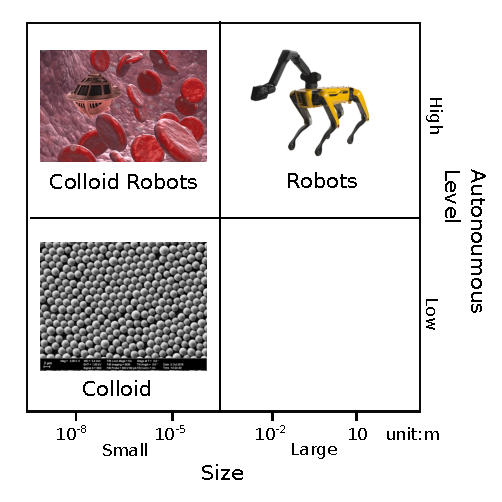
\includegraphics[width=9cm]{figures/1_1.pdf}
\caption{colloidal robots are a combination of the words "colloid" and "robots". colloidal robots are the same size as colloid particles from $\n m$ to$\mu m$ and usually suspend throughout the liquid phase. At the same colloidal robots show dynamics autonomous behaviors such as motion, navigation, and communication, commonly seen in large robotics or living systems}
\label{fig:1.1}
\end{figure}


\section{Essential components for colloidal robots}
Because colloidal robots are still robots, their design shares some of the same basic principles and knowledge from  macroscopic robotic systems.  Traditionally, robots are divided into three essential parts actuators, sensors, and controllers. For example, consider a popular cleaning robot: the Roomba vacuum cleaner (Figure 1.2).  This robot has two actuator systems: one is responsible for locomotion so that the robot can move around your apartment (wheels); the other is responsible for collecting dust and dirt (brush and vacuum).
The sensors for cleaning robots include infrared  sensors and cameras, which provide information about the environment--for example, the position of obstacles. Using such information, the controllers are programmed  to help cleaning robots plan  the actions. For example, if cleaning robots sense a corner, the controllers will let cleaning robots turn around to avoid crashing. One different thing about controllers is that controllers don't necessarily have physical parts. A controller can be a algorithm or a simple math function.  For all the robots, sensor , actuators, and controllers must work together as a feedback loop so robots can work functionally to finish different task: sensors collect information from the environment; based on information from sensors as well as the target of robots,  controllers will make decisions  on how to move actuators; then the actuators will drive robots into a new environment to repeating this feedback loop. This feedback loop composed of actuators, sensors,  and controllers is also the design guidance to build a colloidal robot. However, due to size limitation and different physics regime of colloidal robots, new mechanisms of actuation, sensing and controlling should be developed compared to the conventional approach in the large scale robots.  In the next section, we will address the challenge to build a colloidal robot. 

\begin{figure}
\centering
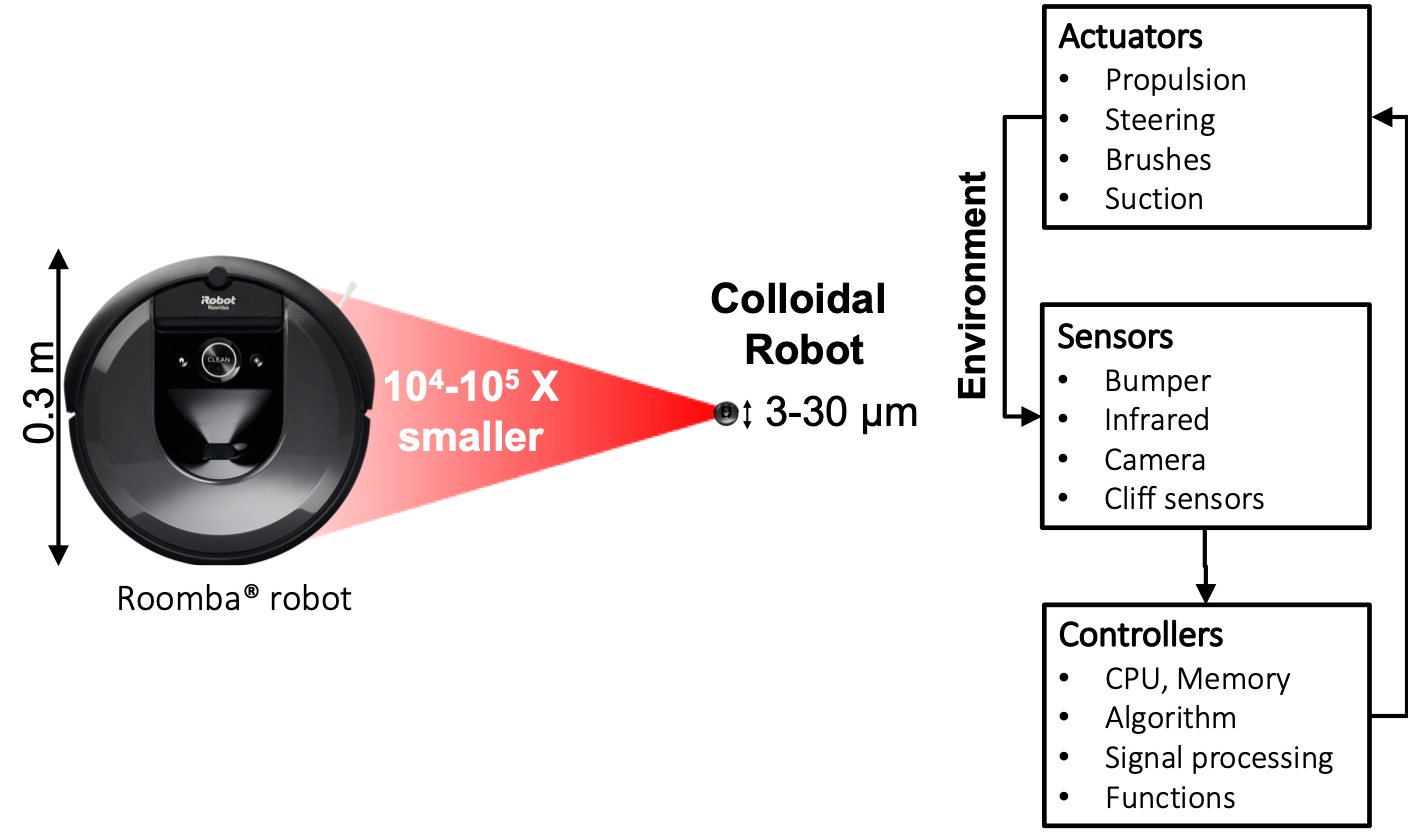
\includegraphics[width=12cm]{figures/1_2.png}
\caption{The essential components and feedback to design a colloidal robot. In the feedback loop, sensors continuously collect information for controllers. Based on  information from sensors and targets of a robot, controllers will make decisions on how to drive the actuators.}
\label{fig:1.2}
\end{figure}

\section{The challenge to  build colloids robots}

\textbf{Size limitation}. In addition to the three basic components (sensors,actuators, and controllers) in the feedback loop, a robot also needs power supplies, manipulators with joints and a body frame, etc. Even for the simplest clean robot, there are around 100 parts inside. It is not possible to integrate all of these complex components in a micron-size particle (a micron size particle on a cleaning robot is just like a human standing on the earth)  if we simply follow the conventional method to build a normal size robot. 

\textbf{Physics limitation}. Physics for a colloid scale particle in the squishy  environment is very different from our normal size world, where everything becomes noisy and sticky. First, in the colloidal scale, Brownian motions largely affect the dynamics of colloidal particles, adding stochastic influence to the robotics. These thermal motions increase the difficulties in controlling the colloidal robot's accuracy and precision. This requires the mechanism to drive colloidal robots to be reliable enough to overcome the background noise. Second, the inertia totally disappears in the small scale as the Reynolds number of the colloidal robot's system approach 0.  The Reynolds number presents the ration of inertia and viscosity represented as
\begin{equation}
    Re=\frac{\rho v l}{\mu}
\end{equation}
where $\rho $ is the density of fluid environment, v is the velocity of particle, l is the size of particle. $\mu$ is the  viscosity of fluid. In the colloid scale, both size and speed of particles are much smaller than 1, leading to the Reynolds number almost 0. The absence of inertia means all of the actuation method in normal size robots based on inertia will no longer work. This interesting  motion restriction in low Reynolds number is called Scallop
theory and was first discussed by Edward Purcell (Professor Prucell was famous for his independent discovery of something else (nuclear magnetic resonance, NMR), which brought him a Nobel prize) \autocite{purcell1977life}. As shown in figure 1.3, Scallop Theorem states that a swimmer which exhibits time-symmetric motion cannot achieve net displacement in a low Reynolds number fluid environment because all the motion is time reversal. There is no difference between closing a scallop and opening a scallop. New actuation methods different large robot systems for colloidal robots must be 

\begin{figure}
\centering
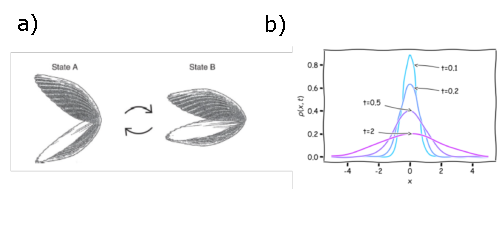
\includegraphics[width=8.5cm]{figures/1_3.pdf}
\caption{Physics challenge for building a colloidal robot (a) Scallop theory. In the colloid scale, the effect of inertia almost disappears, making everything time reversal. (b) Brownian motion. The presence of thermal noise in the colloid scale let the motion of colloidal robots unpredictable.}
\label{fig:1.3}
\end{figure}
To solve the  challenges mentioned above and design the colloidal robots, researchers got inspired from real small living  machines. The dynamic functions of living cells require integration of structures and processes to drive material organization in space and time. For example in the muscle cell,  the coupling of complex structures (kinesin motor protein) and dissipative processes (ATP hydrolysis) can generate mechanical work (see fig 1.4). Thus, a colloidal robot should also have both complex structures and a dissipative process. Thanks to the development of nano/micro scale fabrication in the semiconductor industry, we can now create materials with heterogeneous structure and composition on length scales spanning molecular to macroscopic dimensions with chemical synthesis, lithography, deposition , and etching. These technologies can be directly transplanted to the fabrication process of colloidal robots. In addition to structural and material complexity, the artificial dissipation process (or actuation process) for colloidal robots  can be generated  with chemical reaction, external field (electric, magnetic, acoustic or fluid flow) to generate motion breaking the time reversal constraint. For the past decade, lots of research has been conducted to engineeringly build colloidal robots  or study the fundamentals of colloidal robots. The colloidal robot is now a emerging interdisciplinary field attracting many scientists with different background from math, physics to chemistry, biology and engineering. A state-of-art  review on colloidal robots' research is going to be reviewed in the next section.
\begin{figure}
\centering
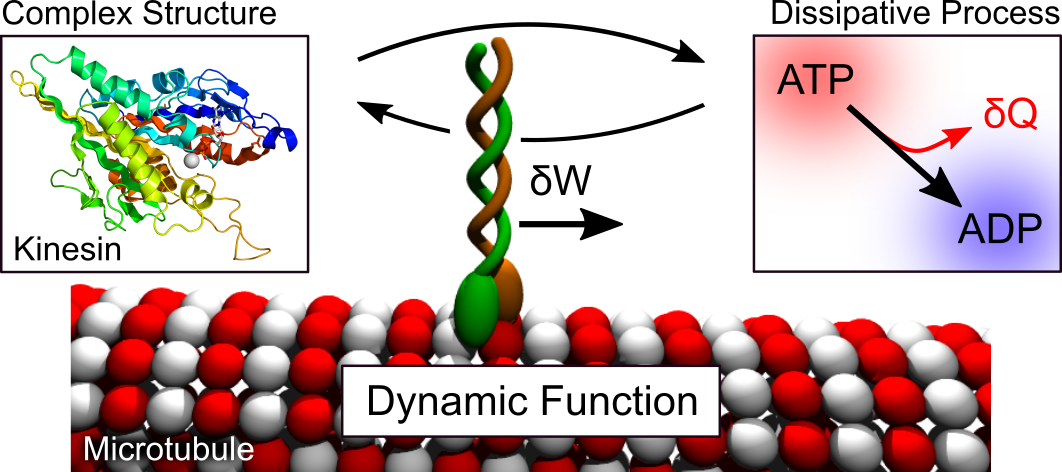
\includegraphics[width=8.5cm]{figures/1_4.png}
\caption{Dynamic functions require the coupling of complex structures and dissipative processes–here, a kinesin motor protein bound to a microtubule  does work powered by ATP hydrolysis}
\label{fig:1.4}
\end{figure}

\section{A state of art review on colloidal robots }
It is not clear which paper first mentioned the similar idea of colloid scale robotics (the original concept of  small scale machines can be tracked to Richard Feynman's famous paper,\textit{There's plenty of room at the bottom}\autocite{feynman1960there}). The current research wave in the past decade on the colloidal robots is triggered by the discovery of self propulsion active colloid particles driven by chemical fuels \autocite{paxton2004catalytic}. In 2004, scientists from Penn State University found that chemical fuel (they use hydrogen peroxide, $H_2O_2$,  in their first paper) can drive  gold-platinum bimetallic nanorods' autonomous motion. The asymmetric different chemical reactions, which happen at the different end of their nanorod,  lead to a net flow fluid near the surface of nanorod. This pioneer research then attracted lots of attention in different research field beyond chemistry such as soft condensed matter physics\autocite{Marchetti2013}, materials science\autocite{han2018engineering}, applied math\autocite{fodor2016far} and engineering \autocite{sitti2015biomedical}. More than tens of thousands of papers related to the autonomous behaviors of colloids have been published since then. However, most of these research papers either experiment or theory only focus on building actuators for colloidal robots. Only a few of them realize some complex tasks with colloidal robots such as navigation. From our knowledge, the higher level's automation is still challenging, and should be the main research direction in the future. In the following content, we are going to give a short state-of-art review on both experiment approach to colloidal robots as well as some basic theories and simulation methods for colloidal robots. In this short review, we have no intention and interest to rephrase and cover all the research papers on colloidal robots like an encyclopedia book. Instead,  I will focus on the main physics, chemistry and engineering ideas behind these papers. 

\subsection{Experiment approach}

\textbf{Fabrication}  High throughput nano/micro scale fabrication technologies in semiconductor manufacturing industry now can make a 3-D structure even smaller than 5 nm \autocite{mokhlesi2010three}. These fancy technologies to make CPU and memory in electronic devices can be transplanted directly to make colloidal robots with almost any desired size, shape and component in cleanroom\autocite{koman2018colloidal}. A typical fabrication process mainly including lithography to make patterns as the main body and frame for colloidal robots , etching to remove unnecessary materials and deposition to introduce new materials. Multi-layer processing can be designed and optimized to make high dimensions and complex structure such as spiral shape\autocite{zhang2009artificial}. After the colloidal robots are fabricated on the wafer, they can be harvested from the silica surface with etching technology or simply physical removal. For the detailed process of fabrication, I would like to refer readers to these three comprehensive reviews\autocite{wong2016synthetic,wang2017emerging, zha2018tubular}. Chemists and material scientists also contributed creative chemical synthesis methods to make colloid scale complex structure with one-pot high-throughput method\autocite{youssef2016shape,gong2017patchy,wang2019active}. One challenge for colloidal robots' fabrication is to   make  colloid scale soft (or shape-shifting) structures with complex components. Liquid crystal, hydrogel gel, droplet, silica polymer and self-assembled nanoparticles are promising candidate materials for micro/nano scale soft structure. \autocite{leong2009tetherless,denkov2015self,zhang2017printing,wei2019molecular}. Another fabrication challenge is to make bio-hybrid colloidal robots which can take advantage of  properties in real living systems. Bio-hybrid colloidal robots require high compatibility  among different materials, where experimental biologists can provide invaluable experience and knowledge\autocite{stanton2016biohybrid,magdanz2013development}.

\textbf{Actuation} Autonomous motion is the most basic characteristic of colloidal robots, making colloidal robots real machines instead of simple colloid particles. colloidal robots can harness energy from the environment and convert energy into mechanical work. Compared to the inertia driven mechanism in normal size robot, the actuation of colloidal robots always experiencing large hydrodynamics resistance force to balance the driving force. The actuation's power source can be divided into two main categories: chemical/biochemical reactions and the external physical fields. Living cells and bacteria use a series of  chemical reaction networks (e.g. ATP hydrolysis) to convert their food source to motions. colloidal robots can also mimic this life-like energy conversion mechanism by implementing the chemical reactions on the surface of colloid particles. The reactions happen between the material of colloidal robots and chemical species in the fluid environment. colloidal robots can work as a catalyst or reactant to trigger the reaction in the fluid environment. For example,  colloidal robots can be made of gold or metal,  which catalysis the hydrogen peroxide in the fluid to water and oxygen. During the fabrication process, these catalysis or reactant material are patterned at different places of colloidal robots to break the symmetry generating chemical species' gradient or reaction product (e.g. bubbles) to actuate colloid particles \autocite{velegol2016origins,shklyaev2016harnessing,parmar2018micro}. Recent reports also showed biochemical reaction (e.g. enzyme) can be options to drive colloidal robot's motions, although the mechanism is still controversial\autocite{zhao2018substrate,somasundar2019positive}.

In addition to  chemical reactions, almost all the external physical field have been used to powering autonomous motion of colloidal robots including electric\autocite{lee2019directed}, magnetic\autocite{zhang2009artificial}, acoustic\autocite{sabrina2018shape}, light\autocite{dai2016programmable}, or thermal field\autocite{lozano2016phototaxis}.  Colloidal robots programmed with physical monopole, dipole or quadrupole will respond to the external physical fields, leading to rotational or transitional motion. For example, colloidal robots can be fabricated with magnetic materials such as nickel and cobalt to a have magnetic dipole moment. Then an external magnetic can generate a torque on the colloid's magnetic moment, manipulating the autonomous motion. Compared to the  chemical reaction actuation method, an external physical field can drive colloidal robots' motion with less fluctuation. \autocite{han2018engineering,ren2018two}. 
The current biggest issue in actuation of colloidal robots is the very low energy efficiency (usually in the order magnitude of $<10^{-5}$ or less). colloidal robots always dissipate large amounts of heat\autocite{wang2013understanding} compared to the real living cells which can perform efficient motion with much less heat dissipation.

\textbf{Coupled actuation}  In addition to a single colloid particle's actuation,  colloidal robots can also be actuated via many actuators' interaction and coupling similar to the multi-cylinder engine in a car. These coupled actuation behaviors can perform some life-like collective functions seen in birds' swarm and fish's flock \autocite{wang2015one,ginot2018aggregation}. Emergent patterns, dynamic clustering, and phase separation have been observed  in different colloidal robot systems. \autocite{buttinoni2013dynamical,ginot2018aggregation,duan2013transition,theurkauff2012dynamic} The interactions among colloidal robots are usually in two forms. One is pure force interaction with each other. For example charged colloidal robots have electrostatics interactions. \autocite{dou2018emergence} The second kind of interaction is indirect influence. One colloidal robot's motion and dynamics  will have an influence on the fluid environment, then  the fluid environment will exert this influence back to other colloidal robots in the same environment. Most of the second type interactions are hydrodynamic or chemical reactions. For example, the hydrodynamics flow induced by one colloidal robots will attract/repel other colloidal robots from it. \autocite{karani2019tuning} Although colloidal robots showing collective behaviors can interact with each other, this kind of communication and interaction is passive and lack of programming. colloidal robots cannot take pre-programmed actions from controllers for some desired tasks when they are exerted on some interactions--most papers studying collective behaviors of colloidal robots only observe the phenomena instead of  programming the dynamics.  As a comparison, in normal size robots research, distributed robotics or  swarms robotics\autocite{wei2010sambot,arvin2014colias} can also show life-like dynamics behaviors, but they are more intelligent. These robots can communicate with the electronic signal instead of pure physics force. They can not only interact with each other, but also perform programmed reactions and different tasks\autocite{rubenstein2012kilobot,rubenstein2014programmable,li2019particle}.

\textbf{Navigation} All the living cells or batteries can sense the information from the environment to navigate themselves for energy, food, or suitable living place called \textit{taxis} behaviors. Autonomous colloidal robots should capable of the same kind of navigation abilities. Not so many experiments approach haven been showed to demonstrate  artificial taxis in colloidal robots compared the large amounts of papers on simply showing autonomous motions. Current approaches mainly belong to two mechanisms: computational vision feedback system and physical force "correction" method. The computational vision feedback system uses a microscope with digital camera to track the location and velocity of colloidal robots online with a computer vision algorithm. Then based on the information of location, speed of colloid particles, and the desired navigation direction, the computer (controllers) will compute the proper external field that should be applied in the next time point. The "tracking-computing-applying new field" feedback loop will continue until colloidal robots reach the destination\autocite{li2017autonomous,han2017sequence} This method has several big defects. The first disadvantage is the size of the whole system. The navigation behaviors have to be coupled with complex external devices (microscope, camera, computer) which is not portable and convenient. Second, this mechanism cannot apply to a large number of colloidal robots with different location and velocity because the external physical field can only satisfy one particle's navigation requirement. The physical force "correction" method can navigate  colloid to transport following  some gradient information mimicking a living taxis behavior. This method uses the local gradient information (e.g.light intensity, chemical species concentration, temperature) or asymmetric geometry to generate torque rotating  the colloidal robot to "correct" its orientation aligning with the gradient. Then the colloidal robot can move along with gradient in the environment showing navigation behaviors \autocite{brosseau2019relating,ten2014gravitaxis,lozano2016phototaxis,baker2019fight} However the physical force correction method  lacks the robotic feedback with controller and sensors. With this mechanism, a colloid particle can only be navigated into one direction, which can't be easily re-programmed for doing other types of navigation tasks in a different environments. All of the problems for the current approach to autonomous navigation mentioned above is due to the lack of sensors and controllers in the colloid scale for colloidal robots





\subsection{Theory and simulation}
Richard Feynman said "What I cannot create, I do not understand." to emphasize the importance of fundamental understanding of science. This is also true for the  research in colloidal robots. To design a colloidal robot of higher automation level, understanding the physics and mathematics behind it is as  important as  experimental attempts. colloidal robots are operated far from the equilibrium state with constant energy and mass flow. Recently years there has been intensively research on non-equilibrium matter, called active matter, in the community of soft matter and statistic physics. Some study is focusing on building a generally high-level theoretical physics framework for active matter with continuum mechanics or statistical mechanism. \autocite{stenhammar2013continuum,solon2015pressure,fodor2016far}. Lots of papers are also trying to use simulation or toy models to discover and design new dynamics behaviors in colloidal robots. \autocite{bechinger2016active,speck2014effective,ten2011brownian}. In this section,  basic physical features and mathematical descriptions are going to be reviewed for colloidal robots.  Deeper and detailed derivation can be referred to our citations.

\textbf{Brownian motion} colloidal robots' motion is influenced by the thermal noise (Brownian motion) in the fluid environment because of their small size. The Brownian motion can be described with Einstein–Smoluchowski Diffusion Equation\autocite{islam2004einstein}. If we take the colloidal robot as  a rigid spherical body, the translation and rotation diffusion coefficients are: 

\begin{equation}
    D_T=\frac{k_B T}{6 \pi \eta R }
\end{equation}
\begin{equation}
    D_R=\frac{k_B T}{6 \pi \eta R^3 }
\end{equation}
where $k_B$ is the Boltzmann constant, $T$ is temperature of the environment, and $\eta$ is the viscosity of fluid, $R$ is the radius of colloidal robots. The diffusion characteristic time is the 
reciprocal of diffusion coefficient, as  $\tau=D^{-1}$. As the size of colloidal robots decrease, the rational diffusion coefficients$D_T$ increase much faster than transnational diffusion coefficients$D_R$. For an actuated colloid with autonomous motion velocity as $v$ in two dimensions, the dynamics can be described as,
\begin{equation}
    \frac{dx}{dt}=v Cos(\theta)+\sqrt{2 D_T}\xi_x, \quad \frac{dy}{dt}=v Sin(\theta)+\sqrt{2 D_T}\xi_y,\quad
    \frac{\theta}{dt}=\sqrt{2 D_R}\xi_\theta
\end{equation}
Where $\xi$ is the independent noise with mean as $0$ and correlation as $\delta(t)$. In chemical engineering, we use the Péclet number to represent the dimensionless ratio between convection  and diffusion. For colloidal robots, the Péclet is 
\begin{equation}
    Pe\propto\frac{v}{\sqrt{D_T D_R}}
\end{equation}
to characterize the influence of Brownian motion on the actuated autonomous motion.

\textbf{Actuated force} As introduced in the previous section, actuation mechanisms are divided into chemical reactions and physical field actuation. For the chemical reactions driven colloidal robots, the phoretic interaction  model describes the system very well. \autocite{golestanian2007,najafi2004simple,golestanian2005propulsion,golestanian2019phoretic} In this model, the reaction rates are considered much faster than the diffusion rate of chemical species, resulting in the following   
quasi-stationary reaction-diffusion equation,
\begin{equation}
    -D\nabla^2 C=0
\end{equation}
where D is the diffusion coefficient of reactant, this is the Laplace equation for concentration in the fluid environment. The boundary condition for this Laplace equation is  colloidal robots' consuming or producing chemical species as,
\begin{equation}
    -D \texbf{n}\cdot \nabla C|_{r=r_s}=\alpha(r_s)
\end{equation}
where $r$ is the distance from the center of colloid, $r_s$ is the radius of colloid, \texbf{n} is the normal vector on the surface of colloid and $\alpha(r_s)$ is the flux rate. The chemical reaction will lead to a net normal flux(denoted as $\alpha(r_s)$ ) on the surface of colloid. The fluid will response to the local gradient change near the colloids and generate a slip velocity as,
\begin{equation}
    v_s=\mu(r_s)(\textbf{I}-\textbf{n}\textbf{n})\cdot \nabla C(r_s)
\end{equation}
$\mu$ is called mobility measuring the response rate of fluid to the concentration gradient. By making $\alpha$ and $\mu$ positive or negative, the asymmetric chemical activity on the surface can lead to autonomous motion.  Also, both repulsion and attraction forces between colloids can be achieved to study collective behaviors of this system. \autocite{michelin2015autophoretic}

For the external physical field actuation, the force exerted on each component colloidal robot following the corresponding law of physics. For example, charged colloidal robots with charge amount $q$ experienced electrostatic force $Eq$ in the electric field $E$; magnetic colloid with dipole $m$ in a magnetic field $B$ can be actuated with torque $m\times B$.
Then we can calculate the total force and torque on the rigid body colloidal robots via doing the surface integration if the force is exerted on the surface.
\begin{equation}
    F=\oint_S f_e \,dS
\end{equation}
\begin{equation}
    T=\oint_S (x-x_c)\times f_e \,dS
\end{equation}
Where $f_e$  is the component of the actuated force and $x_c$ is the center of colloidal robots.

\textbf{Hydrodynamics}  The in-compressible viscous fluids are governed by Navier–Stokes equations without any inertia component as discussed in the previous section,
\begin{equation}
    \eta \nabla^2\textbf{u}-\nabla p=0,\quad \nabla \cdot u=0
\end{equation}
where $\eta$ is the viscosity, p is the pressure from fluid. Although hydrodynamic problems are the most complex ones in modeling colloidal robots because of non-linear terms, it is also the most interesting modeling research part with lost of  nontrivial and unexpected results and patterns. \autocite{Lauga2009,berke2008hydrodynamic,lauga2011life} In the low Reynolds number regime, the hydrodynamic force will balance the external force generated by the actuation mechanism. Stokesian dynamics are used to calculate the  translation and angular velocity of colloidal robots \autocite{Brady1988a,Kim2005}
\begin{equation}
    \left[ \begin{array}{c} F \\ T \end{array} \right] = \begin{bmatrix} A & B \\ B^T & C \end{bmatrix} \left[ \begin{array}{c} v \\ \omega \end{array} \right]
\end{equation}
where \textbf{A}, \textbf{B}, and \textbf{C} are tensors determined only by the shape and orientation of the colloidal robots. The whole big matrix is called resistance tensor, which can be calculated analytically\autocite{Kim2005}  Tensor \textbf{B} is called coupling tensor to couple the transition and rotation together. Resistance tensor is no longer symmetric if boundary exists in the fluid environment.  Stokesian dynamics  can be extended to calculate the hydrodynamics interactions between each other via Faxen's law.
\begin{equation}
    F_{drag}=6 \pi \eta a((1+\frac{a^2}{6}\nabla^2)v_{\infty}(0)-U)
\end{equation}
Where $F$ is the   force exerted by the fluid on the colloid particles, $a$ is the size of colloid, $u$ is the  the translation  velocity of the colloid and $v$ is the disturbance velocity caused by the presence of other colloids in the fluid environment. We would rather direct our readers to James Swan's paper for the full expression of hydrodynamic interaction in the form of Stokesian dynamics. \autocite{swan2011modeling} Basically, the simulation of colloidal robots' dynamics are solving partial differential equations either numerically or analytically with the physical model showed above. In addition to some commercial multiphysics simulation software such as COMSOL\textregistered, there are also some open-access library written in various coding languages  can help to simulate the dynamics of colloidal robots. \autocite{glaser2015strong,anderson2008general,swan2011modeling,singh2019hydrodynamic}

\textbf{Design and optimization} For engineering purposes, colloidal robots should be designed with desired functions\autocite{liebchen2019optimal}. As shown in figure 1.6 the design process should start with constructing and understanding the design parameters space. For example how many physics variables(e.g size, temperature, fluid viscosity, choice of materials) should be added into our design space. And then we  need to reduce the dimension of the design space based on physics and mathematics to make then design problems easier. Dimension reduction is a very essential part of the colloidal robot's design problem. A good dimension reduction will significantly reduce the time searching for the optimized result. Then we build a physical model to link these design parameters and our target functions of colloidal robots together. This physical model should be adequate enough  to capture call the key physics affecting the dynamics of colloidal robots. At the same time, this model should be concise enough to eliminate unnecessary computation work. After the forward modeling is constructed, we can reverse design the parameter of colloidal robots by defining the desired performance functions such as the highest velocity, lowest efficiency. Then the final step is to use an optimization algorithm to find the optimal parameters in the design space for the reverse problems. \autocite{ward1963hierarchical,nocedal2006numerical} Recent research also shows that machine learning technology can assist to design colloidal robots with impressive efficiency\autocite{yang2020micro,yang2020cargo,yang2019deep,tsang2018self}.
\begin{figure}
\centering
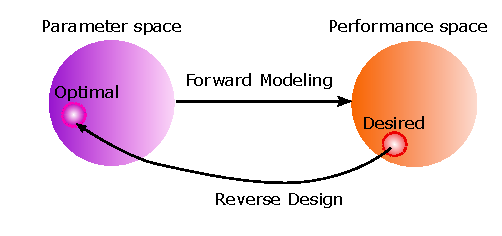
\includegraphics[width=8.5cm]{figures/1_6.pdf}
\caption{The forward modeling connects the design space and performance of colloidal robots together. With the reverse design, the optimal parameters to build a colloidal robot with the desired function can be found.}
\label{fig:1.6}
\end{figure}


%\textbf{Potential Application }


%%%%%%%%%%%%%%%%
% Chapter 2
%%%%%%%%%%%%%%%%

\chapter{Directed motion of metallodielectric particles by contact charge electrophoresis}


%%%%%%%%%%%%%%%%%%%%%%%%%%%%%%
\section{Introduction}

Self-propelled colloidal particles harness energy from their environment to power directed motions relative to their fluid surroundings \cite{Ebbens2015,Li2016,Dey2016}.
Inspired by the locomotion of micro-organisms \cite{Lauga2009}, these artificial swimmers are actively pursued for their potential to navigate complex environments \cite{Takagi2014,Das2015} and deliver cargo to targeted locations\cite{Gao2015,Baylis2015}.
Fluid flows induced by particle motions can also serve to enhance rates of mass transfer to/from the particle surface with emerging applications in water remediation\cite{Soler2013,Li2014} and chemical detection\cite{morales2014micromotor,kagan2009chemical}.
When many self-propelled particles get together, they often interact to form dynamic assemblies\cite{Wang2015} such as swarms\cite{Ibele2009,Nguyen2012}, flocks \cite{Bricard2013}, clusters\cite{JieZhang2016}, and crystals \cite{Palacci2013}.
Synthetic realizations of such active matter\cite{Marchetti2013} provide useful models by which to explore the many forms of self-organization that arise outside of thermodynamic equilibrium.
Importantly, the diverse behaviors of motile particles depend critically on the specific mechanism of self-propulsion and on the associated interactions among the particles.
Expanding the repertoire of colloidal self-propulsion can therefore enable the discovery of new dynamical behaviors as well as the development of future applications.

A wide variety of physicochemical mechanisms have been applied to power the self-propulsion of colloidal particles.
Self-phoretic mechanisms\cite{Golestanian2007} use asymmetries in particle shape and/or composition to create local gradients in the electric potential\cite{Brown2014}, chemical composition\cite{Howse2007}, or temperature\cite{Jiang2010} that drive particle motions via interfacial phoretic effects such as electrophoresis, diffusiophoresis, or thermophoresis, respectively\cite{Anderson1989}.
In a classic example\cite{Paxton2004,Fournier-Bidoz2005}, bimetallic nanorods move autonomously through a homogeneous liquid containing a suitable chemical fuel via reaction-induced  self-electrophoresis\cite{Wang2006,Moran2010}. 
Self-propelled motions of asymmetric particles can also be powered by external fields.
Alternating electric fields drive motions of polarizable particles by induced charge electrophoresis \cite{Squires2006,Gangwal2008,Boymelgreen2014}; alternating magnetic fields power the swimming of flexible magnetic particles by inducing non-reciprocal beating motions \cite{Dreyfus2005}; acoustic fields propel dense metallic particles by directing steady streaming flows\cite{Wang2012,Nadal2014,Ahmed2015}. 
These examples of field-driven particle motion are generally considered forms of self-propulsion, as they allow particles to move freely in multiple directions (typically those perpendicular to the applied field).
The use of external fields to power such motions is attractive for studies of active matter as their magnitude is tunable in space and time.

Here, we describe a type of colloidal self-propulsion in which an electric field drives the autonomous motion of metallodielectric Janus particles\cite{Perro2005,Pawar2008} within an insulating liquid between two plane electrodes (Fig.~\ref{fig:1}a).
Similar configurations have been used to investigate particle motions powered by induced charge electrophoresis within conductive liquids\cite{Boymelgreen2014} and by Quicke rotation within weakly conductive liquids \cite{Bricard2013}.
By contrast, field-driven  motion of conductive particles in insulating liquids is driven by contact charge electrophoresis (CCEP) whereby particles acquire charge on contact with a biased electrode and then move in the field emanating from that electrode \cite{drews2013ratcheted,cartier2014microfluidic,drews2015contact}.
In one well studied example, a conductive sphere immersed in mineral oil oscillates rapidly between two electrodes subject to a constant voltage \cite{drews2015contact}.
Each time the particle contacts an electrode, it acquires charge of opposite polarity and moves back towards the other electrode thereby transporting charge down the applied potential gradient.
Harnessing these motions for useful functions requires strategies by which to rectify particle oscillations.
One approach is to modify the electrodes with asymmetric, ratchet-like features that enable directed transport of conductive particles\cite{drews2013ratcheted} or droplets\cite{Um2016}.
Here, we introduce an alternative strategy that relies on particle asymmetries to achieve similar directed motions.

We show that oscillations of Janus particles between two parallel electrodes are accompanied by steady motions directed perpendicular to the applied field.
Through experiment and theory, we develop and validate a mechanism of self-propulsion whereby the field-induced rotation of the particle upon charge reversal at the electrode surface results in its net displacement during each oscillation cycle.
Repeated displacements in a common direction propel Janus particles at speeds of up to $600~\mu\text{m/s}$ along wide circular arcs within the plane of the electrodes.
Beyond the dynamics of individual particles, we show how particles can both attract or repel one another depending on their separation and on the phases of their respective oscillations.
Together, these results demonstrate how particle symmetry can be used to direct the motions of active colloids powered by CCEP.
The ability to engineer the motions of individual particles and their assemblies will ultimately contribute to the realization of colloidal machines that organize and operate autonomously to perform useful functions \cite{Spellings2015}.

\begin{figure}[p]
\centering
\includegraphics[width=9cm]{2_1.pdf}
\caption{ (a) Schematic illustration of the experimental setup. A metallodieletric Janus particle is immersed in mineral oil between two parallel ITO electrodes (left).  Application of a constant voltage $V$ results in the oscillatory motion of the particle via contact charge electrophoresis (CCEP; right). (b) When imaged from above, the particle moves in and out of focus in time as it oscillates between the electrodes. (c) Over many oscillation cycles, the particle moves steadily away from its conductive hemisphere (top); the steady motion of the particle continues over hundreds of microns (bottom).  See supporting videos 1, 2, and 3.}
\label{fig:1}
\end{figure}
 
 
%%%%%%%%%%%%%%%%%%%%%%%%%%%%%%
\section{Experimental Section}

In a typical experiment, a dilute suspension of Janus particles in mineral oil was sandwiched between two parallel  electrodes separated by a distance $H= 50 - 250~\mu\text{m}$ (Fig.~\ref{fig:1}a). 
We used two types of Janus particles: $8~\mu\text{m}$ silica particles and $4~\mu\text{m}$ fluorescent polystyrene particles, each coated on one hemisphere by a thin layer of gold.
In the absence of an applied field, the particles settled to the surface of the lower electrode where they were imaged from above by an optical microscope.
Application of a constant voltage $V = 200 - 1000~\text{V}$ caused the particles to oscillate rapidly between the electrodes, as evidenced by their periodic appearance and disappearance from the focal plane (Fig.~\ref{fig:1}b). 
Each time a particle came into focus, its position was displaced slightly from that in the previous cycle.
The magnitude and direction of these displacements was relatively constant from one cycle to the next resulting in steady particle motions perpendicular to the applied field.
Using high speed imaging, we quantified the frequency $f$ of particle oscillations as well as the particle position $(x_p,y_p)$ at each oscillation cycle.
For example, at $V = 400~\text{V}$ and $H=200~\mu\text{m}$, a silica Janus particle oscillated between the electrodes at an average frequency of $f = 29~\text{Hz}$ and moved perpendicular to the field at an average speed of $U_{\perp} = 25~\mu\text{m/s}$ (Fig.~\ref{fig:1}c).
Directed particle motion continued over large distances for as long as the voltage was applied.

\subsection{Synthesis of Janus Particles}

Silica Janus particles were prepared by  deposition of gold onto particle monolayers supported on glass slides.
Following Prevo and Velev \cite{prevo2004controlled}, $10~\mu\text{L}$ of a concentrated (30 wt\%) suspension of $8~\mu\text{m}$ silica particles in water was placed between two acid-cleaned microscope slides mounted at an angle on a motorized stage (Harvard Apparatus PHD 2000).
The trapped colloidal solution was dragged at a prescribed speed by the motion of the top slide to achieve well-packed monolayers.
Successive layers of metal (5 nm Ti and 10 nm Au) were then deposited by physical vapor deposition (Cressington 308).

Fluorescent Janus particles were prepared following a procedure adapted from Kopelman et al. \cite{Sinn2011}.
Briefly, sulfonated fluorescent polystyrene particles (ThermoFisher F8858) were washed three times in water by centrifugation and dispersed in methanol at a concentration of 1\% w/v. 
0.5 ml of the particle suspension was deposited onto a 4-inch silicon wafer wafer by spin coating at 2500 rpm for 15 second. 
Successive layers of metal (5 nm Ti, 25 nm Ni, and 20 nm Au) were then deposited by e-beam evaporation (Kurt J Lesker Co. Lab 18). 
The nickel layer was included for a purpose unrelated to the present experiments and is unnecessary here. 
The particles were gently brushed off the wafer using a damp brush.

\subsection{Electrode Configuration}

The electrode setup was comprised of two transparent  indium tin oxide (ITO)-coated glass slides (SIGMA-Aldrich, CAS:50926-11-9, surface resistivity 70-100 $\Omega$/sq) separated from one another by spacers made of glass ($150~\mu\text{m}$ to $250~\mu\text{m}$ thick cover slides) or polydimethylsiloxane (PDMS, $50~\mu\text{m}$ to $100~\mu\text{m}$ thick).
The ITO electrodes were connected to a high-voltage source (Keithley 2410) with a limiting current of $10~\mu\text{A}$ to prevent damage to the system in the event of a short-circuit.
The Janus particles were dispersed in Nylon membrane-filtered mineral oil (SIGMA-Aldrich, CAS:8042-47) at a concentration of $0.01-1~\text{mg/ml}$ and injected into the inter-electrode region.
We note that the charge relaxation time for mineral oil is considerably larger the the timescale of particle oscillations, which is a necessary condition for CCEP \cite{cartier2014microfluidic}. 
The field-induced motion of the Janus particles was captured by a high speed camera (Phantom V310) mounted on an optical microscope (Zeiss Axio Imager A1) operating in bright field mode with 10x and 50x objectives.

\subsection{Particle Tracking}

Movies were captured at frame rates of 1,000 -- 5,000 fps and processed in MATLAB to analyze particle oscillations and reconstruct particle trajectories. 
To determine the oscillation frequency, we first identified a fixed window around a single particle and computed the window-averaged pixel intensity for each frame.
This average intensity oscillated in time as the particle moved into and out of focus, reaching its local minimal value when the particle came into focus at the lower electrode.
For each oscillation cycle $i=1,2,\dots, N$, we identified the time $t_i$ when the particle contacted the lower electrode. 
The mean oscillation frequency was then computed by dividing the number of particle oscillations by the total observation time, $f= N / (\Sigma_i t_i)$.
To reconstruct particle trajectories $(x_i,y_i)$, we considered only those frames when the particle was in focus (i.e., when the average intensity was in local minimum) and determined the location of the particle center using standard algorithms \cite{Track}.
The net displacement for cycle $i$ was computed as $\Delta_i^2 = (x_{i+1} - x_i)^2 + (y_{i+1}-y_i)^2$; the average speed of the particle (parallel to the electrodes) was computed as $U_{\perp} = (\Sigma_i \Delta_i)  /  (\Sigma_i t_i$).

\subsection{Simulation of CCEP Motions}

The model of CCEP dynamics combines classical electrostatics and low Reynolds number hydrodynamics \cite{drews2015contact}. 
The metallic hemisphere of the Janus particle as well as the bounding electrodes are treated as perfect conductors.
To facilitate our numerical analysis, the conductive portion of the particle is modeled as a solid hemisphere with rounded corners (radius $0.1a$) in contrast to the thin hemispherical cap present in experiment.
Additionally, the non-metallic hemisphere and the surrounding fluid are assumed to be dielectrics with a common permittivity $\varepsilon$.
Given the particle charge $q$, orientation $\alpha$, and height $z_p$ above the electrode surface, we solve the Laplace equation numerically to determine the electric potential $\Phi$ and field $\ve{E}=-\nabla \Phi$ throughout the dielectric medium (see Supporting Information for details).
We then integrate the Maxwell stress over the surface of the conductive hemisphere to determine the electric force and torque that drive particle motion.

At low Reynolds numbers (in experiments $Re\leq0.01$), the translational and rotational velocities of the particle are linearly related to the external force and torque by the so-called resistance tensor \cite{Kim2005, Swan2007}.
For a spherical particle near a solid plane boundary, there exist exact analytical expressions \cite{Kim2005} for the components of this tensor, which, when suitably rescaled, depends only on the separation between the sphere and the plane. 
Using these expressions, we compute the particle velocity and integrate numerically to determine the position and orientation of the particle as a function of time.
We assume that the charge $q$ on the particle remains constant until the surface of the metallic hemisphere reaches some critical separation $\delta$ from the plane electrode, at which point charge flows to/from the particle instantaneously to reverse the particle polarity ($q\rightarrow -q$).
Physically, the contact charging process is thought to occur by a type of dielectric breakdown; the resulting charge on the particle is somewhat variable but consistently less than that expected at equilibrium (i.e., when the potential on the particle equals that of the electrode) \cite{drews2015contact}.
After nondimensionalization, the computed particle trajectories depend on just two parameters: the dimensionless charge $q / 4\pi\varepsilon a^2 E$ and the dimensionless separation at contact $\delta / a$.


%%%%%%%%%%%%%%%%%%%%%%%%%%%%%%
\section{Results and Discussion}

Figure \ref{fig:2}a shows the reconstructed trajectories of six different Janus particles under identical conditions over the course of one hundred oscillation cycles based on the experiment results. 
The cumulative displacement of each particle increased roughly linearly with the number of oscillations (Fig.~\ref{fig:2}b) as the particles moved along wide circular arcs of radius $30~\mu\text{m}$ or greater.
These observations are consistent with the spatial homogeneity of the applied field, which suggests that particle motion be invariant to translation and rotation in the $xy$ plane of the electrodes.
Although the majority of particles (ca.~70\% for $V=800~\text{V}$ and $H=200~\mu\text{m}$) exhibited such directed motions, some Janus particles were observed to oscillate between the electrodes with no lateral motion whatsoever.
Additionally, some particles (ca.~20\%) remained ``stuck'' to the electrode surface and did not move at all upon application of the field.

For the particles that moved, the oscillation frequency increased monotonically with increasing voltage as $f \propto V^{2}$ (Fig.~\ref{fig:2}c).
This observation is consistent with previous studies of CCEP motion, which showed that the oscillation frequency scales as $f\sim\varepsilon a V^2 / \eta H^3$, where $\varepsilon$ and $\eta$ are the permittivity and viscosity of the fluid, respectively, and $a$ is the particle radius \cite{drews2015contact}.
By contrast, the lateral displacement of the particle during each oscillation cycle was largely independent of the applied voltage; each oscillation contributed an average displacement of $\Delta = 0.2 a$ (Fig.~\ref{fig:2}d).
Consequently, the lateral velocity of the particle, $U_{\perp}\equiv f\Delta$, also increased as the square of the applied voltage (Fig.~\ref{fig:2}e).
This velocity could be further increased by decreasing the spacing between the electrodes $H$ to increase the magnitude of the applied field (Fig.~\ref{fig:2}f). 
Using spacers of $H=50~\mu\text{m}$, we observed particles velocities up to $U_{\perp}=600~\mu\text{m/s}$ in the direction perpendicular to the applied field.


\begin{figure}[p]
\centering
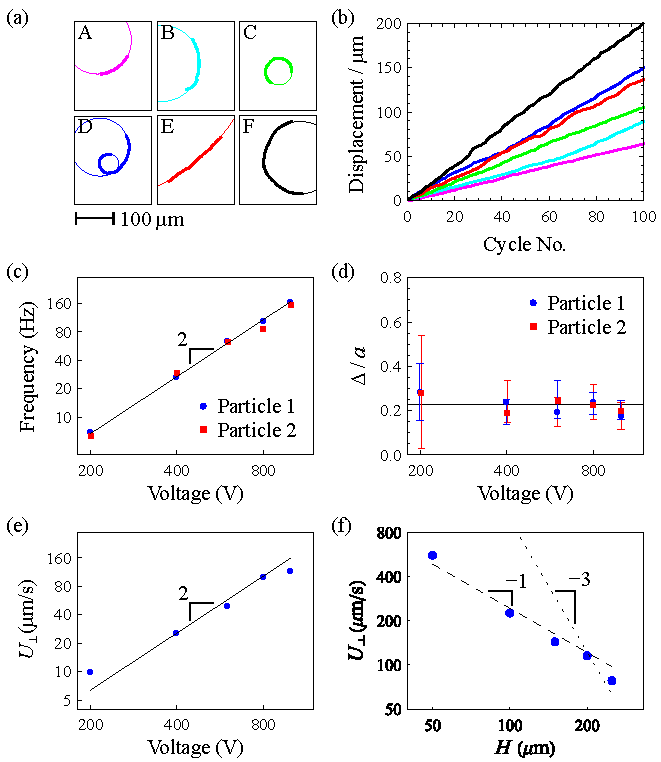
\includegraphics[width=11.2cm]{2_2.pdf}
\caption{(a) Reconstructed particle trajectories of six Janus particles (radius $a = 4~\mu\text{m}$; voltage $V=800~\text{V}$; electrode spacing $H=200~\mu\text{m}$).  Markers denote the particle position at successive oscillations; curves are best circular fits to the data. (b) The cumulative displacement of particles in (a) increases linearly with the number of oscillation cycles. (c) The oscillation frequency of the particle scales quadratically with the voltage.  Markers show data for two independent particles with an electrode spacing $H=200~\mu\text{m}$; the curve is a fit of the form $f\propto V^2$. (d) The lateral particle  displacement $\Delta$ during each oscillation is largely independent of the applied voltage. Markers show the mean displacement; error bars denote one standard deviation above and below the mean. (e) The particle velocity perpendicular to the field scales as the square of the voltage. Markers show data for one particle with an electrode spacing $H=200~\mu\text{m}$; the curve is a fit of the form $U_{\perp}\propto V^2$. (f) Particle velocity increases with decreasing electrode spacing. Each marker represents the velocity of a single particle for an applied voltage $V=800~\text{V}$.}
\label{fig:2}
\end{figure}

To explain these experimental observations, we propose the following propulsion mechanism illustrated in Figure \ref{fig:3}a. 
As it moves across the channel, a charged Janus particle adopts a preferred orientation in which its principal axis is oblique to the applied field and its motion is directed towards the metallic hemisphere.
When it contacts either electrode, the charge on the particle changes sign thereby altering its preferred orientation in the field.
The field-induced rotation of the particle in the vicinity of the electrode surface results in a lateral displacement, which is qualitatively similar to that of a sphere ``rolling'' along the surface.
Successive rotations occur in a common direction towards the non-metallic hemisphere causing a steady lateral motion over the course of many oscillations.
This putative mechanism is supported both by experimental observations of the transient particle orientation and by a mathematical model that describes the electrostatics and hydrodynamics of CCEP motion.

\begin{figure}[p]
\centering
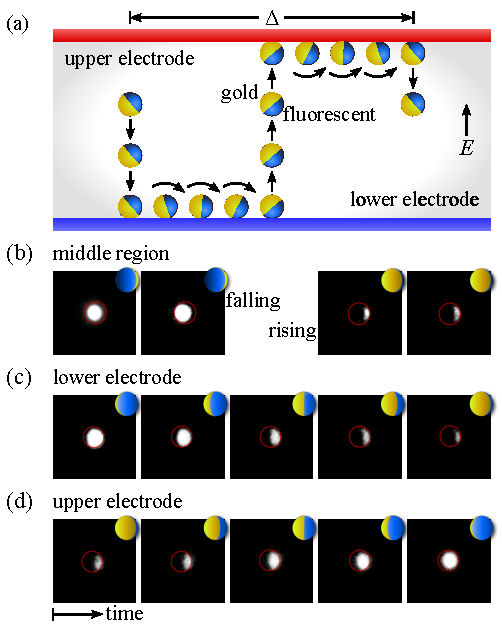
\includegraphics[width=8.5cm]{2_3.pdf}
\caption{(a) Schematic illustration of the propulsion mechanism showing one oscillation cycle.  Rotation of the particle near the electrodes results in a lateral displacement $\Delta$. (b-d) Fluorescent microscopy images highlight the non-metallic hemispheres of fluorescent Janus particles. Images are captured from above; the icons show the particles viewed from above using the color scheme from (a). Particles in the middle region (b) adopt a stable orientation that depends on their direction of travel (falling vs.~rising). Upon contacting the lower (c) or upper (d) electrode, particles rotate in time from one orientation to another. See supporting video 4.}
\label{fig:3}
\end{figure}

We used fluorescent particles to better visualize the orientation of Janus particles moving by CCEP.  
Such particles appeared bright when the metallic hemisphere was directed ``down'' (negative $z$ direction; away from the microscope objective) and dark when the metallic hemisphere was directed ``up'' (positive $z$ direction; towards the objective). 
For intermediate orientations, the fluorescent hemisphere of the particle was partially visible like the bright side of the moon in different phases.
By focusing on planes in the middle of the two electrodes, we observed that particles moving downward appeared bright (gibbous moon) while those moving upward appeared dark (crescent moon) (Fig.~\ref{fig:3}b).
By focusing on the lower electrode, we directly observed the rotation of the particle as it transitioned from the gibbous to crescent configuration (Fig.~\ref{fig:3}c).  
The opposite behavior was observed at the upper electrode where the particle rotated from the crescent to gibbous configuration (Fig.~\ref{fig:3}d).
Importantly, the orientation of the Janus particle in the plane of the electrodes remained relatively constant from one cycle to the next, which allowed the particle to move steadily away from its metallic hemisphere.   

To gain further insights into the propulsion mechanism, we use the equations of classical electrostatics and low-Reynolds number hydrodynamics to describe the dynamical trajectories of Janus particles moving by CCEP.
We first consider the case of a single Janus particle with a net charge $q$ in an unbounded medium subject to a uniform electric field $E$.
We solve for the electric potential within the dielectric and evaluate the electrostatic torque $L(\alpha)$ on the particle as a function of its orientation $\alpha$ relative to the field.
For each charge, there exists one stable orientation for which the electric torque is zero $L(\alpha)=0$ and its derivative is negative $L'(\alpha)<0$ (Fig.~\ref{fig:4}a).
Uncharged Janus particles tend to orient perpendicular to the applied field owing to the increased polarizability of their metallic hemisphere in that orientation ($\alpha=\pi/2$ for $q=0$).
The addition of positive or negative charge, respectively, acts to rotate the particle towards or away from the direction of the field.
When the charge exceeds a critical magnitude, the particle orients perfectly with or against the applied field.
Importantly, this critical charge is similar in magnitude to that acquired by the particle during contact charging (see Fig.~S2). 

\begin{figure}[p]
\centering
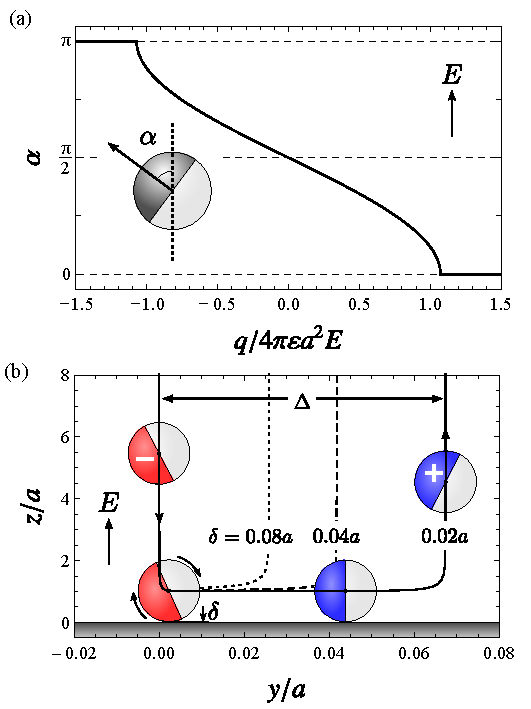
\includegraphics[width=9cm]{2_4.pdf}
\caption{Results of the theoretical model. (a) The stable orientation $\alpha$ of a Janus particle in a uniform electric field depends on the particle's charge $q$ (scaled by $q_s = 4\pi\varepsilon a^2 E$). Uncharged particles align perpendicular to the applied field $E$ ($\alpha=\pi/2$ for $q=0$); highly charged particles align parallel to the field ($\alpha=0,\pi$ for $|q|>1.07 q_s$). (b) Simulated particle ``collisions'' with the lower electrode for a particle charge $q=\pm0.5q_s$. The solid curve shows the trajectory of the particle center; the orientation of the particle at different points along the trajectory is illustrated graphically. The net particle displacement $\Delta$ depends on the surface separation $\delta$ at contact when the particle charge reverses polarity. Note that for clarity the $z$ and $y$ axes use different scales.}
\label{fig:4}
\end{figure}

We now consider the dynamics of a particle ``collision'' with the lower electrode (Fig.~\ref{fig:4}b). 
Initially, the particle is positioned far from the electrode surface ($z_p\gg a$) with some fixed charge $q$. 
We solve for the electrostatic force and torque on the particle and compute the translational and rotational particle velocity in proximity to the surface.
We then integrate these dynamical equations of motion to describe the position and orientation of a single particle as function of time.
Figure \ref{fig:4}b shows three different particle trajectories for different contact separations and a common charge $q = 0.5 q_s$ where $q_s = 4\pi\varepsilon a^2 E$ is a convenient charge scale.
The trajectories are in qualitative agreement with the experimental observations: a particle moves towards the electrode with a preferred orientation, reverses its charge on contact, rotates and translates as it adopts a newly preferred orientation, and ultimately moves away from the surface.
The net lateral displacement $\Delta$ depends on how closely the particle approaches the surface.
For particles that approach more closely to the surface, their rotational motion is more tightly coupled to their lateral translation, and they move farther during each collision.
The displacement also depends on the particle charge in an somewhat surprising way: highly charged particles ($q > q_s$) exhibit little or no displacement (Fig.~S6).
Such particles contact the surface with their axis aligned parallel with field and therefore experience little or no torque upon charge reversal.
Instead, these particles move backward from the surface before ultimately rotating into the new stable orientation; particle rotation far from the surface, however, results in little or no lateral displacement.
This prediction of the model provides a plausible explanation for those particles that oscillate but do not translate perpendicular to the field.

There are some experimental observations that are not captured by the idealized model.
Notably, the model predicts that particles should move along straight lines and not the circular trajectories observed in experiment.
We attribute this discrepancy to defects on the Janus particles that break their axial symmetry.
Imperfections in the particles' metallic hemispheres are known to arise during metal deposition due to shadowing by neighboring particles \cite{Pawar2008}.
Such defects can lead to electric torques about the principle axis of the particle, which are otherwise prohibited by symmetry.
As a result, particles are permitted to change their orientation in the plane of the electrode upon charge reversal.
Understanding these effects requires further study of non-axisymmetric particles of well defined shape.
Interestingly, in some experiments, the curvature of the particle trajectory changed abruptly during its motion (e.g., particle D in Fig.~\ref{fig:2}a). 
This observation may imply that non-axisymmetric particles are capable of multiple ``modes'' of self-propulsion; however, we cannot yet dismiss alternative explanations based on adventurous dust particles.

As noted above, the propulsion velocity is equal to the product of the oscillation frequency and the rotation-induced displacement: $U_{\perp}=f\Delta$.
This expression suggests two basic strategies for maximizing the particle velocity: (i) increase the oscillation frequency, $f\sim\varepsilon a V^2/\eta H^3$, or (ii) increase the lateral displacement upon charge reversal.
The oscillation frequency can be enhanced by increasing the voltage or by decreasing the spacing between the electrodes (Fig.~\ref{fig:2}e,f).
Of course, the electrode spacing cannot be smaller than the particles themselves, and the electric field cannot exceed the dielectric strength of mineral oil (ca.~$5~\text{V/}\mu\text{m}$).
In Figure \ref{fig:2}f, the applied field actually exceeds this threshold value for electrode spacings less than $H=200~\mu\text{m}$; however, device failure was avoided by limiting the current to only $10~\mu\text{A}$.
Under these conditions, the electric field remains roughly constant, and the velocity scales as $U_{\perp}\propto H^{-1}$ (not $U_{\perp}\propto H^{-3}$ as expected for a constant voltage). 
To increase the rotation-induced displacement of the particle on charge reversal, it is necessary to alter the geometry of the particle itself (e.g., the size of the metallic patch). 
Such modifications can be challenging to achieve in practice and their consequences difficult to anticipate. 
Ultimately, the magnitude of the displacement is limited by the size of the particle ($\Delta < a$).

Beyond the motions of individual particles, we observed several interesting  behaviors in systems of two or more interacting particles (Fig.~\ref{fig:5}).
When two particles were separated by a distance less than the electrode spacing ($d<H$), they influenced one another at a distance through electrostatic interactions.
These interactions were either attractive or repulsive depending on the respective phases of the particle oscillations\cite{mersch2011antiphase}.
Like-charged particles oscillating ``in phase'' repelled one another as evidence by an increase in particle separation with time (Fig.~\ref{fig:5}a).
By contrast, oppositely-charged particles oscillating ``out of phase'' moved toward one another in time (Fig.~\ref{fig:5}b).
Due to slight differences in their oscillation frequencies, two particles often transitioned repeatedly between attractive and repulsive regimes.
This particle ``dance'' could end in two different ways: either the particles moved off in different directions to find new partners, or they embraced one another to form a dynamic oscillating chain (a so-called bucket brigade \cite{Pelesko2004a}).
Finally, we observed that interacting particles often moved together in a common direction -- typically, along the line connecting the particle centers (Fig.~\ref{fig:5}c).
Such coordinated motions were considerably faster that the propulsion velocity of individual Janus particles perhaps suggesting an additional strategy for directing CCEP motions.
Importantly, we confirmed that the above effects involving two or more particles were also observed among spherically isotropic (non-Janus) particles.
Understanding the complex dynamics of multiple particles moving by CCEP will require further study beginning with the simplest spherical particles.

\begin{figure}[p]
\centering
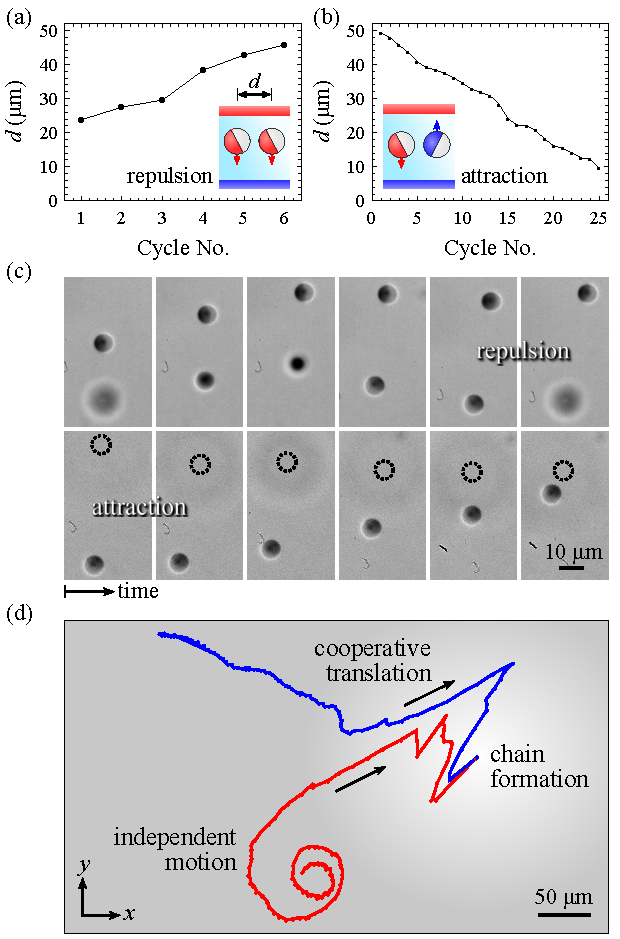
\includegraphics[width=10.5cm]{2_5.pdf}
\caption{(a) The horizontal distance $d$ between two particles oscillating in phase increases during each oscillation cycle. (b) The distance between particles moving out of phase decreases each cycle. (c) Image sequence corresponding to data shown in (a) and (b). (d) Reconstructed trajectories for two interacting particles.  Initially, the particles are moving independently until their separation becomes less than the electrode spacing (here, $H=150~\mu\text{m}$). They then begin to move more quickly in a cooperative manner.  Ultimately, the particles come together to form an oscillating chain. See supporting video 5.}
\label{fig:5}
\end{figure}



%%%%%%%%%%%%%%%%%%%%%%%%%%%%%%
\section{Conclusions}

Contact charge electrophoresis drives the rapid oscillatory motion of conductive microparticles within nonpolar fluids.
Particle asymmetries can be used to rectify such oscillatory motions to achieve directed transport perpendicular to the applied field.
Rectified motions derive from particle rotations near the electrode surface upon contact charge transfer, which lead to repeated displacements in a common direction.
This type of self-propulsion exhibits several characteristics that distinguish it from related systems based on self-phoresis, induced-charge electrophoresis, or Quicke rotation.
Owing to the negligible electric currents through the nonpolar fluid, particle motions are highly efficient and require small energy inputs (ca.~1 nW / particle) \cite{drews2015contact}. 
Rapid particle motions can enhance microscale mixing within nonpolar fluids \cite{cartier2014microfluidic}, which could be harnessed to accelerate catalytic reactions limited by mass transfer.
Long-ranged electrostatic interactions among the particles results in complex collective motions relevant to the study of active matter.
Importantly, the directed CCEP motions of asymmetric particles can in principle be engineered by tuning the particle shape and surface composition.
The rational design of such active components is a critical prerequisite for constructing dynamic colloidal assemblies capable of useful functions -- that is, colloidal machines.


%%%%%%%%%%%%%%%%%%%%%%%%%%%%%%









%%%%%%%%%%%%%%%%
% Chapter 3
%%%%%%%%%%%%%%%%

\chapter{Emergence of traveling waves in linear arrays of electromechanical oscillators}




%%%%%%%%%%%%%%%%%%%%%%%%%%%%%%%%%%%
%%%%%%%%%%%%%%%%%%%%%%%%%%%%%%%%%%%
%%%%%%%%%%%%%%%%%%%%%%%%%%%%%%%%%%%
\section{introduction}
Traveling waves of mechanical actuation provide a versatile strategy for locomotion and transport in both natural and engineered systems across many scales. These rhythmic motor patterns are often orchestrated by systems of coupled oscillators such as beating cilia or firing neurons. Here, we show that similar motions can be realized within linear arrays of conductive particles that oscillate between biased electrodes through cycles of contact charging and electrostatic actuation. The repulsive interactions among the particles along with spatial gradients in their natural frequencies lead to phase locked states characterized by gradients in the oscillation phase. The frequency and wavelength of these traveling waves can be specified independently by varying the applied voltage and the electrode separation. We demonstrate how traveling wave synchronization can enable the directed transport of material cargo. Our results suggest that simple energy inputs can coordinate complex motions with opportunities for soft robotics and colloidal machines.

Traveling waves of mechanical actuation provide a versatile strategy for locomotion and transport in both natural\autocite{Cohen1982, Blake1974, Taylor447} and engineered\autocite{Ijspeert2008, Palagi2016, Park2016, Masuda2016, Yashin2012} systems across many scales. In vertebrates such as the aquatic lamprey \autocite{Cohen1982, Cohen1992}, these and other rhythmic motor patterns are orchestrated by networks of neurons called central pattern generators (CPGs) \autocite{Marder2001}, which are often idealized as systems of coupled oscillators \autocite{Cohen1982, Cohen1992}. The rhythmic output of these oscillators is relayed to actuators (e.g., muscles) to produce complex motions without the need for sensory feedback. Similar control strategies based on CPGs are used to direct  locomotion in macroscopic robots \autocite{Ijspeert2008}. At smaller scales, however, it becomes increasingly challenging to accommodate centralized control systems capable of directing the coordinated actions of multiple actuators. Instead, microorganisms such as ciliated protozoa integrate pattern generation and mechanical actuation within a single material system.  The oscillatory motions of beating cilia couple to one another through hydrodynamic interactions to produce metachronal waves that drive cellular locomotion through viscous surroundings \autocite{Blake1974, Niedermayer2008, Elgeti2013}. This biological example illustrates how the coupled motions of many mechanical oscillators can organize spontaneously and autonomously to perform dynamic functions.

The realization of synthetic systems that mimic such functions requires experimental strategies for powering mechanical oscillators and for coupling their motions to achieve the desired dynamics. One approach relies on coupling reaction-diffusion patterns to the mechanical deformation of responsive gels, for example, to achieve traveling wave motions in excitable media\autocite{Yashin2012,Masuda2016}. Despite fascinating demonstrations of this approach on millimeter length scales, it remains challenging to miniaturize due to the need for faster reactions that compete with diffusion at smaller scales. To achieve scalable mechanisms of pattern formation, the processes that drive oscillations should scale in the same way as those used to couple neighboring oscillators. In this context, electromechanical oscillators based on contact charge electrophoresis (CCEP) \autocite{bishop2018contact, drews2015contact} can provide a useful model on length scales spanning millimeters\autocite{Mersch2011} to microns\autocite{Dou2016} (perhaps even nanometers \autocite{Park2000,Kowalik2016}). 

CCEP refers to the back-and-forth motion of a conductive particle \resp{through an insulating fluid separating} two electrodes subject to a constant voltage. \resp{The particle charges on contact with either electrode and moves down the applied potential gradient, thereby transporting charge between the biased electrodes. This type of electromechanical oscillator is fundamentally distinct from the weakly damped harmonic oscillators of micro-electromechanical systems (MEMS)\autocite{van2011review,Zhang2014}, which rely on resonant excitation by time-varying fields. By contrast, CCEP oscillators are powered by a constant thermodynamic driving force and operate even under conditions of strong damping, which arise at small scales and in viscous environments.  Similar to those of molecular motors\autocite{Kolomeisky2007,Kowalik2016}, CCEP motions can be rectified to perform mechanical work or to transport material cargo\autocite{drews2013ratcheted,Kowalik2016}. Moreover,} the charge acquired by the particle and the forces driving its motion are well described by classical electrostatics, which is invariant to changes in scale. The discovery of new CCEP motions at the macroscale is therefore transferable to emerging applications at the microscale\autocite{bishop2018contact}.

Here, we investigate the collective dynamics of many CCEP oscillators positioned along a linear array between two (nearly) parallel electrodes (Fig.~\ref{fig:1}a). Each oscillator is comprised of a conductive sphere that moves back and forth between the electrodes along a dielectric track.  Oscillatory motions are driven by the repeated charging of the particles on contact with either electrode and their subsequent movement in the applied field. The dynamics of neighboring oscillators are coupled to one another through the electrostatic interactions between the charged particles. We show how this electrostatic coupling mediates the organization of phase-locked states in which all oscillators move with a common frequency. Interestingly, the distribution of oscillator phases at steady state corresponds to traveling waves of particle motion with a characteristic wavelength comparable to the electrode separation. These experimental observations are explained by a Kuramoto-like model\autocite{Acebron2005,Tsimring2005} that accounts for weak repulsive coupling between neighboring phase oscillators and for small systematic variations in their natural frequencies. We demonstrate how traveling wave synchronization can be used to transport material cargo along the length of the oscillator array. More generally, our approach shows how simple energy inputs can power complex patterns of mechanical actuation, which may be useful in powering the motions of soft robots\autocite{rus2015design, acome2018hydraulically} and colloidal machines\autocite{Snezhko2011,Yan2012, Martinez-Pedrero2015, goodrich2017using, Driscoll2017}.

%%%%%%%%%%%%%%%%%%%%%%%%%%%%%%%%%%%
\begin{figure}[p!]
    \centering
    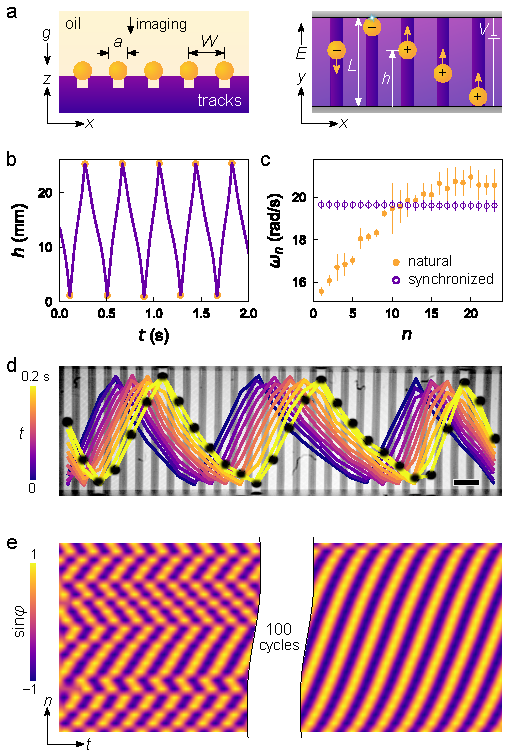
\includegraphics[width=10cm]{3_1.pdf}
    \caption{\textbf{Travelling wave synchronization.} (a) Conductive spheres immersed in mineral oil oscillate along dielectric tracks connecting two plane electrodes subject to a constant voltage $V$. Particles charge on contact with each electrode and move in the electric field $E$. (b) Oscillatory dynamics of a single particle showing its position $h$  as a function of time $t$; yellow markers denote contacts with the electrodes. The applied voltage is $V=19$ kV; the electrode separation is $L=25$ mm. (c) Oscillation frequency $\omega_n$ as a function of the position $n$ along the array. The natural frequency of each oscillator varies with position (solid markers); all oscillators move with a common frequency in the synchronized state (open markers). Error bars represent the standard deviation in the instantaneous frequency, $2\pi/(t_{k+1}-t_k)$, over 100 cycles. (d) Image of the experiment showing particle positions at successive times; scale bar is 3 mm. (e) Space-time plot of the oscillator phase $\varphi$ showing the emergence of traveling wave synchronization for the $N=23$ oscillators in (c) starting from a random initial configuration.  Here, the track period is $W=3$ mm; other parameters are listed in (b).}
    \label{fig:1}
\end{figure}
%%%%%%%%%%%%%%%%%%%%%%%%%%%%%%%%%%%


%%%%%%%%%%%%%%%%%%%%%%%%%%%%%%%%%%%
%%%%%%%%%%%%%%%%%%%%%%%%%%%%%%%%%%%
%%%%%%%%%%%%%%%%%%%%%%%%%%%%%%%%%%%
\section{Results}

\subsection{Experiment}

Copper spheres ($a = 1$ mm in radius) immersed in mineral oil were positioned within an array of dielectric tracks connecting two plane electrodes separated by a distance $L$ (Fig.~\ref{fig:1}a). The tracks were spaced evenly with a period $W=3a$ and aligned perpendicular to the electrode surfaces and to the direction of gravity. Each track contained a single particle, which was free to move back and forth between the two electrodes. Application of a constant voltage (typically, $V=10$ kV) caused the particles to oscillate continuously between the electrodes via contact charge electrophoresis (CCEP) \autocite{bishop2018contact, drews2015contact}. The conductive particles acquired an electrostatic charge on contact with the biased electrodes and moved under the influence of the applied field. This periodic cycle of contact charging and electrostatic actuation continued for as long the voltage was applied.

% Dynamics of individual particles

%\noindent
%\textbf{Dynamics of electromechanical actuator arrays}
Figure \ref{fig:1}b shows the reconstructed trajectory of a single sphere oscillating between the two electrodes. Each time the particle contacts an electrode, its charge changes sign and the particle reverses direction under the influence of the field. To facilitate the analysis of multiple particles over many oscillation cycles, we record the times at which each particle contacts one of the electrodes.  From this data, we approximate the phase of each oscillator by interpolating between successive contacts as $\varphi(t) = 2\pi (t-t_k)/ (t_{k+1}-t_{k})$ where $t_k$ denotes the time of the $k^{th}$ contact and $t_k \leq t < t_{k+1}$. By definition, the oscillator phase increases at a constant rate equal to the natural frequency, $\mathrm{d}\varphi/\mathrm{d}t = \omega$, which is approximated by averaging over many oscillation cycles as $\omega = \langle 2\pi/(t_{k+1}-t_{k}) \rangle_k$. Repeating this analysis for each particle in isolation (i.e., one track at a time), we observed small systematic variations in the natural frequency $\omega_n$ with respect to the oscillator position $n$ along the array (Fig.~\ref{fig:1}c, solid markers). The spatial gradients in the oscillator frequency were caused by small deviations in the electrode alignment,  which was controlled only to within ca.~1$^\circ$ of parallel. Particles oscillated faster where the electrodes were closer together due to an increase in field strength at those locations.
        
% Dynamics of particle arrays
Despite variations in their natural frequencies, linear arrays of $N$ particle oscillators moving simultaneously evolved in time to a phase-locked state, in which each particle moved with a common frequency (Fig.~\ref{fig:1}c). Interestingly, the synchronized particles did not move in phase with one another but rather organized to form a single traveling wave, which remained stable for hundreds of oscillation cycles (Fig.~\ref{fig:1}d; Supplementary Movie 1). Space-time plots of the oscillator phase $\varphi_n(t)$ show how this wave-like pattern emerged from a disordered initial configuration (Fig.~\ref{fig:1}e; see also Supplementary Fig.~1 and Supplementary Movie 2). The direction of wave propagation was related to the spatial gradient in the oscillators' natural frequencies: waves traveled from slower to faster oscillators. Notably, the travelling wave patterns were robust to disturbances and recovered when disrupted by external perturbations (Supplementary Movie 3).

%%%%%%%%%%%%%%%%%%%%%%%%%%%%%%%%%%%
%%%%%%%%%%%%%%%%%%%%%%%%%%%%%%%%%%%
%%%%%%%%%%%%%%%%%%%%%%%%%%%%%%%%%%%

% The role of particle number $N$ 
The stability of the synchronized state and the distribution of oscillator phases therein depended on the number of oscillators $N$ in the array. For $N=2$ oscillators, the particles moved in antiphase as reported previously \autocite{Mersch2011} (Fig.~\ref{fig:2}a). Such antiphase synchronization suggests that neighboring oscillators are coupled together by repulsive interactions such as the Coulombic forces between like-charged particles. As the number of particles was increased, the average phase difference between successive oscillators decreased giving rise to stable traveling waves with wavelengths spanning many oscillators (Fig.~\ref{fig:2}b; see also Supplementary Fig.~2 and Supplementary Movie 4). Beyond some critical number of oscillators $N^*$, the synchronized state became unstable (Fig.~\ref{fig:2}c). Above this threshold, traveling waves were observed to grow and break near the center of the array in a periodic fashion (Supplementary Movie 5). Such breaking events are characterized by dislocation-like defects in the space-time plots for the oscillator phases (Fig.~\ref{fig:2}c). The breaking frequency increased as the number of oscillators was increased beyond the stability threshold $N^*$ (Supplementary Fig.~3). For $N\gg N^*$, wave breaking was no longer periodic but rather occurred at irregular intervals and at different locations (Supplementary Fig.~4 and Supplementary Movie 5).
    
%%%%%%%%%%%%%%%%%%%%%%%%%%%%%%%%%%%
\begin{figure}[p!]
    \centering
    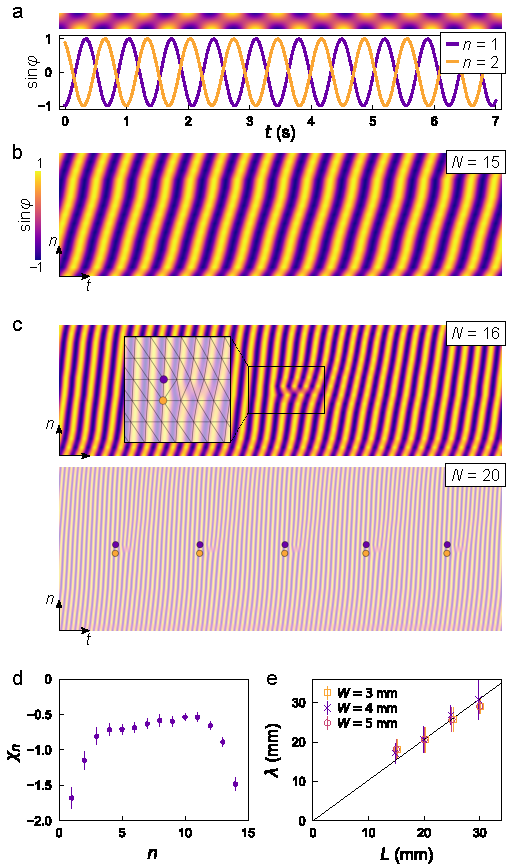
\includegraphics[width=10cm]{3_2.pdf}
    \caption{\textbf{Characterization of travelling waves.} (a) $N=2$ oscillators moving in antiphase. The plot shows the sine of the oscillator phases (bottom); the space-time image shows the same data in a different way (top). (b) Space-time plot for $N=N^*=15$ oscillators showing 20 oscillation cycles. (c) Space-time plots for $N>N^*$ showing defects that occur at regular time intervals. The markers show points in the space-time lattice with five-fold (purple) and seven-fold (yellow) coordination. (d) Time-averaged phase difference $\chi_n$ as a function of position $n$ for $N=N^*$ oscillators. Data for (a-d) were collected with $L=25$ mm, $W=3$ mm, and $V=18$ kV.  (e) Characteristic wavelength $\lambda$ as a function of the electrode separation $L$ for $N=N^*$ and different oscillator spacings $W$. Error bars represent the standard deviation from five independent experiments.}
    \label{fig:2}
\end{figure}
%%%%%%%%%%%%%%%%%%%%%%%%%%%%%%%%%%%

% Characteristic wavelength for $N=N^*$ (Fig.~\ref{fig:3})
To better understand the synchronized state, we quantified the distribution of oscillator phases for $N = N^*$ as a function of the electrode separation $L$ and the oscillator spacing $W$. For each electrode configuration, we started with $N>N^*$ oscillators and removed one particle at a time from the end of the array until reaching a stable synchronized state, at which the phase difference between neighboring oscillators was constant in time. Figure \ref{fig:2}d shows the time-averaged phase difference $\chi^{\s}_n = \langle \varphi_{n+1}(t) - \varphi_n(t) \rangle_t$ at the stationary state for a typical experiment. The phase difference was smallest (in magnitude) near the center of the array and largest near the edges. For each such state, we defined a characteristic wavelength in terms of the average phase difference as $\lambda = 2\pi W / \langle \chi_n^{\s} \rangle_n$. This wavelength increased linearly with the electrode spacing $L$ but was independent of the oscillator spacing $W$ over the range explored (Fig.~\ref{fig:2}e).

%%%%%%%%%%%%%%%%%%%%%%%%%%%%%%%%%%%%%%%
\subsection{Minimal Model of Traveling Wave Synchronization}

The experimental observations are reproduced by a Kuramoto-like model \autocite{Acebron2005} that accounts for the local repulsive coupling between neighboring oscillators and the systematic variations in their natural frequencies.  In the model, we adopt the following simplified description of CCEP dynamics\autocite{Kowalik2016}. \resp{On contact with either electrode, a conductive sphere acquires a charge $q = \pm \tfrac{2}{3}\pi^3\varepsilon a^2 E$, where $E$ is the electric field at the electrode surface, and $\varepsilon$ is the permittivity of the surrounding dielectric.  This expression---first derived by Maxwell\autocite{Maxwell1873}---assumes that charge flows to/from the particle until its potential equals to that of the contacting electrode\autocite{drews2014charge}. The electrostatic force on the particle is approximated as $F = q E$, which drives motion with velocity $U=F/\gamma$, where $\gamma$ is a constant friction coefficient. Figure \ref{fig:4}a shows how the charge $q$ and position $h$ of a single oscillator depend on its phase $\varphi=\omega_{\ro} t$, where $\omega_{\ro} = \pi q_{\ro} E_{\ro}/\gamma L$ is the natural frequency defined in terms of the applied field $E_{\ro}=V/L$ and the Maxwell charge $q_{\ro}=\tfrac{2}{3}\pi^3\varepsilon a^2 E_{\ro}$. By comparing the measured frequency in Fig.~\ref{fig:1}c to the prediction of the model, the friction coefficient can be estimated to be $\gamma=1.8\times10^{-3}$ N s m$^{-1}$, which ca.~4 times larger than the Stokes drag, $\gamma_{\text{s}}=6\pi\eta a$. The increased drag is attributed to the solid boundaries formed by the patterned tracks and the planar electrodes (Supplementary Fig.~5)\autocite{Goldman1967a}.}

% Interactions 
\resp{The presence of neighboring oscillators influences both the charge that a particle acquires and the speed at which it moves.  To describe these interactions, we decompose the electric field as $E=E_{\ro}+E'$, where $E_{\ro}$ is the applied field and $E'$ is a disturbance field due to neighboring particles, which are approximated as point charges (see Methods). In the limit of weak interactions (i.e., when $E'\ll E_{\ro}$), the moving particles are well approximated as phase oscillators with weak repulsive coupling between nearest neighbors.} The phase of the $n^{\text{th}}$ oscillator evolves in time as
\begin{equation}
    \frac{\partial \varphi_n}{\partial t} = \omega_n + f(\varphi_n - \varphi_{n-1}) + f(\varphi_n - \varphi_{n+1}), \label{eq:phase}
\end{equation}
where $\omega_n$ is the natural frequency, and the function $f(~)$ describes the phase-averaged interactions between neighboring oscillators as a function of their phase difference $\chi_n=\varphi_{n+1}-\varphi_n$. The boundaries of the array are open such that oscillators at the edges ($n=1,N$) interact with only one neighbor \autocite{Ottino-Loffler2016}. We assume a uniform gradient in the natural frequency:  $\omega_n = \omega_{\ro} +  \Delta \left[n-\tfrac{1}{2}(N+1)\right]$ for $n=1\dots N$, where $\omega_{\ro}$ is the mean oscillator frequency, and $\Delta$ is the frequency difference between successive oscillators due to a small angle $\theta$ between the electrodes ($\Delta/\omega_{\ro} \approx 3(W/L)\theta  \ll 1$).  Interestingly, this model was investigated previously as a possible explanation for traveling wave oscillations in the central pattern generator of the aquatic lamprey \autocite{Cohen1982}. 

%%%%%%%%%%%%%%%%%%%%%%%%%%%%%%%%%%%
\begin{figure}[p!]
    \centering
    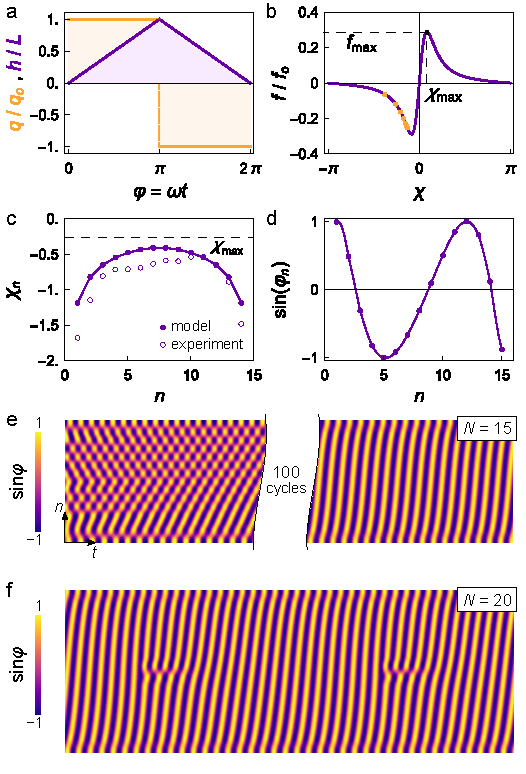
\includegraphics[width=10cm]{3_3.pdf}
    \caption{\textbf{Minimal model of traveling wave synchronization.} (a) Charge $q$ and position $h$ of a idealized oscillator as a function of it phase $\varphi$. \resp{(b) Phase-averaged electrostatic interaction between two weakly-coupled oscillators as a function of their phase difference $\chi$. The interaction is scaled by $f_{\ro} = q_{\ro}^2/\varepsilon W^2 L \gamma$; the oscillator spacing is $W=0.12 L$. (c) Stable stationary solution for the phase difference $\chi_n$ of $N=15$ oscillators. Experimental data for the same conditions is reproduced for comparison. The predicted phase differences are plotted also in (b) to show their relationship with the interaction function $f(~)$. (d) Sine of the oscillator phase $\varphi_n$ showing the wave-like pattern.  (e) Dynamics of the $N=15$ oscillators starting from random initial conditions. (f) Oscillator dynamics for $N=20$ showing the periodic breaking of the traveling waves. In (c)--(e) the critical oscillator number is chosen to be $N^*=15.5$ as in experiment, which implies a frequency gradient $\Delta=0.0096 f_{\ro}$. The natural frequency is $\omega_{\ro}=\tfrac{3}{2\pi^2}(W/a)^2f_{\ro}=1.4 f_{\ro}$ where $W/a=3$ as in experiment; the ratio $\Delta/\omega_{\ro}=0.0070$ implies an electrode angle of $\theta=1.1^{\circ}$.}}
    \label{fig:4}
\end{figure}
%%%%%%%%%%%%%%%%%%%%%%%%%%%%%%%%%%%

% Description of the electrostatic interactions
In the present context, the primary interaction between neighboring oscillators is electrostatic in origin; other interactions are neglected. In particular, the neglect of hydrodynamic interactions was supported by experiments in which neighboring particles were separated by solid walls without altering their collective dynamics (Supplementary Fig.~6).  Approximating the particles as point charges, we compute the electrostatic interaction averaged over one oscillation cycle for a constant phase difference $\chi$ (see Methods). These repulsive interactions are described by an odd function characterized by the location $\chi_{\max}$ and height $f_{\max}$ of its maximum  (Fig.~\ref{fig:4}b).  For large electrode separations ($L\gg W$), these quantities are well approximated as $f_{\max}\approx \tfrac{1}{2\sqrt{3}} (q_{\ro}^2/\varepsilon W^2 L \gamma)$ and $\chi_{\max}\approx\tfrac{\pi}{\sqrt{2}} (W/L)$. \resp{Our assumption of weak coupling implies that the phase velocity due to interactions is small compared to the natural frequency---that is, $f_{\max}\ll\omega_{\ro}$ or, equivalently, $a/W\ll0.72$. Additional simulations incorporating the full amplitude dynamics provide further support for the phase oscillator approximation under the experimental conditions of $a/W=0.33$ (Supplementary Note 1 and Supplementary Fig.~7).}

% Stationary states of the minimal model
The competition between the repulsive interactions and the frequency gradient leads to stable stationary solutions described by $f(\chi_n) = -\frac{1}{2}\Delta n(N-n)$ (see Methods). This solution exists provided that the number of oscillators is below some critical value $N^* = \sqrt{8 f_{\max}/\lvert\Delta\rvert}$. Figure \ref{fig:4}c,d,e shows the stable solution in terms of the phase difference and the sine of the phase for $N=15$ oscillators---just below the chosen critical value of $N^*=15.5$. The addition of more particles ($N>N^*$) causes the waves to break periodically in the center of the array (Fig.~\ref{fig:4}f). Physically, faster oscillators pile up behind the slower ones and are prevented from passing by the local repulsive interactions.  In this way, the frequency gradient acts to compress the oscillator phases together to create longer waves that travel always from slower to faster oscillators. When compression by the frequency gradient exceeds the repulsive barriers between neighboring oscillators, global synchronization is lost and the waves break. 

At the critical oscillator number ($N = N^*$), repulsive interactions are at their maximum ($\chi^{\s}_n \sim \chi_{\max}$), and the characteristic wavelength scales linearly with the electrode separation in agreement with experimental observations (Fig.~\ref{fig:2}e)---that is, $\lambda\sim2\pi W/ \chi_{\max} \sim L$ for $W\ll L$.  Moreover, the critical oscillator number observed in experiment implies a certain angle between the electrodes, which can be estimated from the model as $\theta = \tfrac{1}{3}(L\Delta /W \omega_{\ro} ) = \tfrac{8 \pi ^2}{9 \sqrt{3}} (a^2 L/W^3 {N^*}^2)$. For the conditions of Figure \ref{fig:2}, this angle is predicted to be $\theta = 1.1^\circ$, which agrees well with that measured from the experimental images (Fig.~\ref{fig:1}b).  Smaller angles allow for stable waves containing more particles. 

The average phase within the wave evolves in time at a constant rate equal to the average frequency $\omega_{\ro}$, which is specified independently of the wavelength. In experiment, the oscillator frequency could be altered by changing the applied voltage; however, the range of accessible frequencies was limited by dielectric breakdown at higher voltages and by particle sticking at lower voltages\autocite{drews2015contact}. Notably, the frequency of the phase locked state was slightly faster than the average natural frequency (Fig.~\ref{fig:1}d). Dipolar interactions among the particles (neglected here) break the odd symmetry of the interaction function thereby altering the frequency of the synchronized state.


%%%%%%%%%%%%%%%%%%%%%%%%%%%%%%%%%%%
%%%%%%%%%%%%%%%%%%%%%%%%%%%%%%%%%%%
%%%%%%%%%%%%%%%%%%%%%%%%%%%%%%%%%%%
\section{Discussion}

We have shown how arrays of electromechanical oscillators can organize spontaneously to form synchronized traveling waves of particle motion powered by a constant input voltage.  The direction of wave propagation is determined by small gradients in the natural frequencies of the oscillators and can be controlled by introducing a small angle between the otherwise parallel electrodes.  The characteristic wavelength is approximately equal to the electrode separation $L$ and corresponds to the largest possible wave that can be stabilized by repulsive interactions among the charged particles.  The traveling wave motions are robust to perturbations and can be harnessed to direct the transport of material cargo.  In particular, Figure \ref{fig:5}a shows how traveling waves can direct the motion of gas bubbles floating at the interface just above the oscillating particles (see also Supplementary Movie 6).  Bubbles are transported in the direction of wave propagation at speeds comparable to the wave velocity (Fig.~\ref{fig:5}b). In contrast to previous strategies for rectifying CCEP motions based on ratcheted channels\autocite{drews2013ratcheted} or asymmetric particles\autocite{Dou2016}, the present approach relies on the self-organization of multiple particles working in concert. 

%%%%%%%%%%%%%%%%%%%%%%%%%%%%%%%%%%%
\begin{figure}[h]
    \centering
    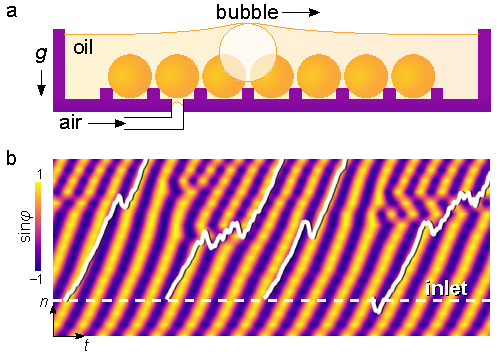
\includegraphics[width=10cm]{3_4.pdf}
    \caption{
    \textbf{Transport of air bubbles via travelling waves.} (a) Schematic illustration of the experimental set-up from the side. (b) Trajectories of four bubbles (white) superimposed over the space-time plot of the oscillator phase. See also Supplementary Movie 6.}
    \label{fig:5}
\end{figure}
%%%%%%%%%%%%%%%%%%%%%%%%%%%%%%%%%%%

\resp{Beyond this initial demonstration, traveling wave synchronization of CCEP oscillators may be useful for peristaltic pumping within microfluidic systems. Unlike standard pressure pumps, those based on traveling wave motions allow for recirculating flows\autocite{mi5020289} and would complement existing  applications of CCEP in microfluidic cargo transport\autocite{drews2013ratcheted,cartier2017electric}, separations\autocite{drews2013ratcheted}, and fluid mixing\autocite{cartier2014microfluidic}. These CCEP-powered unit operations rely on constant voltages at low input power, which makes them attractive for use in portable, battery-powered microfluidic devices\autocite{bishop2018contact}.  One important limitation of these oscillators is their reliance on the dielectric environment provided by non-polar fluids; CCEP motions cannot be sustained in even weakly conductive liquids such as deionized water\autocite{cartier2014microfluidic}. However, recent advances in soft robotics suggest one strategy for circumventing this limitation by encapsulating non-polar liquids in stretchable, impermeable compartments\autocite{acome2018hydraulically}. These soft composite materials can be deformed by applying voltages to stretchable electrodes patterned on their surfaces.  By incorporating arrays of CCEP oscillators within such dielectric compartments, it should be possible to create self-organized motions that drive transient deformations and thereby locomotion of soft robotic materials. } 

%%%%%%%%%%%%%%%%%%%%%%%%%%%%%%%%%%%
%%%%%%%%%%%%%%%%%%%%%%%%%%%%%%%%%%%
\section{Methods}

%%%%%%%%%%%%%%%%%%%%%%%%%%%%%%%%%%%
\paragraph{Experiment Set-up.} 
Periodic arrays of dielectric tracks were 3D printed in acrylonitrile butadiene styrene (ABS) with a period of $W=3-5$ mm. The array was sandwiched between two copper plates separated by a distance $L=10-30$ mm (McMaster-Carr 3350K201) and immersed in mineral oil (Sigma Aldrich CAS No.~8042-47-5). The tracks were aligned perpendicular to the electrode surfaces and to the direction of gravity. Each track contained a single copper sphere (McMaster-Carr No.~64715K16, radius $a=1$ mm), which rolled freely between the two electrodes (Fig.~\ref{fig:1}a). Prior to use, the system was heated in a 60$^\text{o}$C oven for several hours to remove any moisture. The copper electrodes were connected to a amplifier (Trek 20/20C) with an output voltage $V=0-20$ kV.  The particles were illuminated from below by a light emitting diode (LED) and their motions captured by a high-speed camera (Phantom V310).  During each experiment, the electrodes were energized to a specified voltage and the resulting particle motions captured. The voltage was switched off for at least one minute between successive experiments to allow for the dissipation of any space charge accumulated on the surfaces of the tracks and/or the electrodes.  Particle location data were extracted using standard image tracking routines in MATLAB.


%%%%%%%%%%%%%%%%%%%%%%%%%%%%%%%%%%%
\paragraph{Bubble Transport.} 
Bubbles were generated within the oscillator array by a continuous flow of air supplied by a syringe pump at a rate of 0.2 ml min$^{-1}$. The air was delivered through a tube that connected to a hole in the base of one of the tracks (Fig.~\ref{fig:5}a).  The bubbles (ca.~4 mm in diameter) were transported down the length of the array by the coordinated motions of $N=17$ particles of radius $a=1.5$ mm (Supplementary Movie 6).  In these experiments, the applied voltage was $V=18$ kV, the electrode separation was $L=20$ mm, and the height of the mineral oil above the base of the track was 4 mm.  Bubbles were always transported in the direction of wave propagation, which was controlled by introducing a finite angle between the two electrodes.  Control experiments with no applied voltage showed no bubble motion in either direction.


%%%%%%%%%%%%%%%%%%%%%%%%%%%%%
\paragraph{Electrostatic Interactions.}
We first consider a single point charge $q$ positioned at a height $z=h$ between two grounded planes at $z=0$ and $z=L$.  The resulting electrostatic potential at point $\ve{x}$ is 
\begin{equation}
    \phi(\ve{x}) = \frac{q}{\pi L \varepsilon} \sum_{m=1}^{\infty} \sin\left(\frac{m\pi h}{L}\right)  \sin\left(\frac{m\pi z}{L}\right) K_0\left(\frac{m \pi r}{L}\right),\label{eq:point}
\end{equation}
where $r=\sqrt{x^2 + y^2}$ is the radial distance from the charge, and $K_0(~)$ is the zeroth order modified Bessel function of the second kind. For large arguments, the Bessel function decays exponentially as $K_0(s)\rightarrow e^{-s}\sqrt{\pi/2 s} $; the infinite series can be truncated for some $m\gg L/\pi r$ to obtain an accurate approximation.  The corresponding electric field in the $z$-direction is given by $E_z = -\partial \phi / \partial z$. 

\resp{We now consider how the disturbance field $E'$ due to one oscillator $i$ influences the dynamics of another oscillator $j$ in the limit of weak coupling. At zeroth order in $E'$, the phase of each oscillator increases at a constant rate $\omega_{\ro}$ such that $\varphi_i=\omega_{\ro} t$ and $\varphi_j=\omega_{\ro} t+\chi$, where $\chi=\varphi_j-\varphi_i$ is the constant phase difference.  The charge $q=q(\varphi)$ and position $h=h(\varphi)$ of each oscillator depends on the phase as shown in Figure~\ref{fig:4}a. At first order in $E'$, the disturbance in the phase of oscillator $j$ evolves as
\begin{equation}
    \frac{d \varphi'_j}{d t} = \frac{\pi n(\varphi_j)}{L\gamma} \left[q(\varphi_j) E'(\varphi_i,\varphi_j) + q'(\varphi_i,\varphi_j) E_{\ro} +\dots\right], \label{eq:j}
\end{equation}
where the factor $\pi n(\varphi_j)/L\gamma$ relates the electric force to the corresponding phase velocity with $n(\varphi_j)=\pm 1$ indicating the direction of travel. The bracketed terms describe two types of electrostatic interactions. First, the disturbance field due to particle $i$ drives particle $j$ to move faster or slower between the electrodes. Using the point charge solution (\ref{eq:point}), this disturbance $E'(\varphi_i,\varphi_j)$ is given by
\begin{equation}
    E'(\varphi_i,\varphi_j) = -\frac{q(\varphi_i)}{L^2 \varepsilon} \sum_{m=1}^{\infty} m \sin\left(\frac{m\pi h(\varphi_i)}{L}\right)  \cos\left(\frac{m\pi h(\varphi_j)}{L}\right) K_0\left(\frac{m \pi W}{L}\right),
\end{equation}
where $W$ is the oscillator spacing. Second, the disturbance field due to particle $i$ alters the charge acquired by particle $j$ on contact with either electrode; the disturbance charge $q'(\varphi_i,\varphi_j)$ is given by 
\begin{equation}
    q'(\varphi_i,\varphi_j) = \begin{cases} 
    +\tfrac{2}{3}\pi^3 \varepsilon a^2  E'(-\chi,0) & 0 \leq \varphi_j < \pi
    \\
    -\tfrac{2}{3}\pi^3 \varepsilon a^2 E'(\pi-\chi,\pi) & \pi \leq \varphi_j < 2\pi
    \end{cases}.
\end{equation}
Physically, the charge on particle $j$ is determined by its most recent contact with either electrode ($\varphi_j=0$ or $\pi$); the field due to particle $i$ at the time of that contact determines the disturbance charge.}

\resp{We can now average these two interactions over one oscillation cycle to obtain the phase-averaged interaction function,
\begin{equation}
    f(\chi) = \frac{\pi}{L\gamma}\frac{1}{2 \pi}\int_0^{2\pi} n(\varphi_j) \left[ q(\varphi_j) E'(\varphi_j-\chi,\varphi_j) + q'(\varphi_j-\chi,\varphi_j) E_{\ro} \right] d\varphi_j.
\end{equation}
Carrying out the integration, each of the two electrostatic interactions produce contributions of the same mathematical form with the second term contributing twice that of the first,
\begin{equation}
     f(\chi) = \frac{3\pi q_{\ro}^2}{2  \varepsilon L^3\gamma} \sum_{m=1}^{\infty} m \sin(m \chi)  K_0\left(\frac{m\pi W}{L}\right).
\end{equation}
This final expression is plotted in Figure \ref{fig:4}b for the case of $W/L=0.12$. }


%%%%%%%%%%%%%%%%%%%%%%%%%%%%%%%%%%%
\paragraph{Stationary Solution.} 
Starting from Eq.~(\ref{eq:phase}), we recast the oscillator dynamics in terms of the phase difference $\chi_n=\varphi_{n+1} - \varphi_n$ and the average phase $\Phi=\tfrac{1}{N}\sum_n\varphi_n$.  Taking the difference in the phase dynamics of successive oscillators, we obtain the following equation for the phase difference 
\begin{equation}
    \frac{\partial \chi_n}{\partial t} = \Delta - f(\chi_{n-1}) + 2 f(\chi_n) - f(\chi_{n+1})\quad\text{for }n=2,\dots,N-2, \label{eq:diff}
\end{equation}
which makes use of the fact that $f(~)$ is an odd function.  At the open boundaries of the array, the phase difference evolves as
\begin{equation}
    \frac{\partial \chi_1}{\partial t} = \Delta + 2f(\chi_1) - f(\chi_2)\quad\text{and}\quad\frac{\partial \chi_{N-1}}{\partial t} = \Delta - f(\chi_{N-2}) + 2f(\chi_{N-1}). \label{eq:diffBC}
\end{equation}
In addition to these $N-1$ equations, the dynamics of the $N$ oscillators is described by the that of the average phase, $\partial \Phi /\partial t = \omega_{\ro}$, which is fully decoupled from the phase differences. Setting the time derivatives in Eqs.~(\ref{eq:diff}) and (\ref{eq:diffBC}) equal to zero, the resulting recurrence equation can be solved to obtain the stationary solution, $f(\chi_n) = \tfrac{1}{2}\Delta n(n-N)$, presented in the main text. This solution exists provided that $f_{\max}>\tfrac{1}{8}N^2\lvert\Delta\rvert$ (Supplementary Note 2) and is stable when $f'(\chi_n)<0$ (Supplementary Note 3). The characteristic relaxation time for approaching the stationary state is given by the diffusive-like scaling relation $\tau\sim \chi_{\max}N^2/\pi^2 f_{\max}$.




%%%%%%%%%%%%%%%%
% Chapter 4
%%%%%%%%%%%%%%%%

\chapter{Autonomous navigation of shape-shifting microswimmers$^{*}$}
\begin{center}
\vspace*{1\baselineskip}
\textbf{Abstract}
\end{center}

We describe a method for programming the autonomous navigation of active colloidal particles in response to spatial gradients in a scalar stimulus. Functional behaviors such as positive or negative chemotaxis are encoded in the particle shape, which responds to the local stimulus and directs self-propelled particle motions. We demonstrate this approach using a physical model of stimuli-responsive clusters of self-phoretic spheres. We show how multiple autonomous behaviors can be achieved by designing the particle geometry and its stimulus response.

\section{Introduction}\footnotetext[1]{This chapter is adapted from "Dou, Y., & Bishop, K. J. (2019). Autonomous navigation of shape-shifting microswimmers. \textit{Physical Review Research}, 1(3), 032030."}
% Section Headings to be removed
Chemotactic bacteria swim autonomously through complex media to regulate their environment and find new energy sources. Physically, these functional behaviors are enabled by feedback between local sensing and autonomous motion across stimulus landscapes that vary in space and time (Fig.\ \ref{fig:4.1}a). Depending on the relationship between sensing and motion, different functional behaviors can be achieved (e.g., positive or negative taxis, kinesis). In particular, bacteria use temporal sampling and biochemical memory to bias their run-and-tumble motions in even weak gradients, which cannot be detected directly over the length of the organism \autocite{cates2012diffusive}.  

By contrast, attempts to mimic such autonomous propulsion and navigation in synthetic colloids \autocite{bechinger2016active} have relied on particle alignment within stimulus gradients to direct particle motion (e.g., gradients of chemical concentration \autocite{hong2007chemotaxis,popescu2018chemotaxis}, magnetic potential \autocite{Kline2005}, light intensity \autocite{lozano2016phototaxis}, fluid velocity \autocite{Palacci2015}, and fluid viscosity \autocite{liebchen2018viscotaxis}). Such gradients exert mechanical torques on the particle that bias its orientation, thereby enabling directed propulsion---often by a different mechanism. This approach does not scale favorably to micron-scale colloids moving in weak gradients, where the accompanying torques are overwhelmed by Brownian motion. For example, magnetic alignment of a colloid with magnetic moment $\ve{m}$ cannot be achieved when the applied torque is smaller than the thermal energy, $m B\ll k_B T $. Chemotactic bacteria are not subject to this type of constraint as they treat stimulus gradients as sensory cues (i.e., information) rather than sources of mechanical actuation. To create synthetic colloids with similar capabilities, it is necessary to integrate the distinct processes of sensing and actuation to achieve desired functions such as autonomous navigation. The realization of such colloidal robots \autocite{palagi2018bioinspired, han2018engineering} will require strategies by which to systematically `program’ or `encode’ the desired behaviors within the material structure of micron scale particles.
%Moreover, the mechanisms of self-propulsion (e.g., self-phoresis \autocite{golestanian2007designing,popescu2018chemotaxis}) are often re-purposed for navigation, which presents challenges for designing different functional behaviors such as positive \emph{or} negative chemotaxis.  
%The realization of colloidal robots \autocite{palagi2018bioinspired,han2018engineering} that navigate autonomously through fluid environments requires new strategies for programming active particles to bias their motion in response to local stimuli.

Here, we propose one such strategy based on the shape-directed propulsion of shape-shifting microswimmers that alter their shape and thereby their motion in response to changes in a scalar stimulus (e.g., the concentration of a particular chemical species; \resp{Fig.\ \ref{fig:4.1}a}). Particle shape provides a versatile medium for encoding the dynamic behavior of active colloids powered by a variety of energy inputs (e.g., electric \autocite{brooks2018shape}, acoustic \autocite{sabrina2018shape}, self-electrophoretic \autocite{brooks2019shape}). Moreover, by using stimuli-responsive materials, microscale particles can be designed to change their shape in response to environmental cues \autocite{magdanz2014stimuli,palagi2016structured}.  We describe how these two concepts can be integrated to design active colloids that navigate autonomously across heterogeneous stimulus landscapes.   

%\textbf{Model.} % Section Headings to be removed
We consider a single self-propelled particle moving on a two-dimensional domain with linear velocity $\ve{U}=U\cos\alpha \ve{e}_{x'} + U\sin\alpha \ve{e}_{y'}$ and angular velocity $\ve{\Omega}=\Omega \ve{e}_{z'}$ (\resp{Fig.\ \ref{fig:4.1}b}). In the particle frame of reference, the velocity components---parameterized by $U$, $\alpha$, and $\Omega$---depend only on an internal state variable $s\in[0,1]$, which describes a single degree of freedom in the particle shape.  The internal state of the particle depends in turn on the local value of a scalar stimulus field $S(\ve{x},t)$ such as the concentration of a chemo-attractant or repellent.  We assume that the state variable $s$ evolves rapidly to changes in the stimulus and is uniquely determined by its magnitude at the particle center $\ve{x}_p$---that is, $s=f(S(\ve{x}_p,t))$. For a given stimulus landscape $S(\ve{x},t)$, the dynamics of the particle is therefore determined by the response functions, $U(S)$, $\alpha(S)$, and $\Omega(S)$, which describe how particle motion depends on the magnitude of the local stimulus.

\section{Particle Motion in Stimulus Gradients} % Section Headings to be removed
The response functions can be designed to enable particle migration up (or down) spatial gradients in the stimulus landscape. In a homogeneous environment, the particle moves with a constant speed along circular orbits of radius $R=U/\Omega$, larger than the characteristic size of the particle $L$.  Although the particle cannot detect stimulus gradients directly, it can integrate the effects of such gradients over each circular orbit to produce steady motions guided by the gradient. 

For example, a uniform gradient in the $x$-direction, $S(\ve{x})=G x$, causes the particle to drift with velocity $\ve{V}=-\tfrac{1}{2}G U R \alpha' \ve{e}_x + \tfrac{1}{2}G U R' \ve{e}_y + \mathcal{O}(G^2)$, where primes denote differentiation with respect to the stimulus $S$ \autocite{Supp}. To prohibit motion perpendicular to the gradient direction, the radius $R$ of the particle trajectory should be designed to be independent of the stimulus magnitude. Higher order contributions to the drift velocity are negligible provided that drift is much slower than propulsion---that is, when $V\ll U$ or, equivalently, when $G\ll 2/R\alpha'$. With these assumptions, the resulting particle trajectory depends only on the response function $\alpha(S)$, which characterizes the orientation of the propulsion velocity in the particle frame (\resp{Fig.\ \ref{fig:4.1}c}).

Fig.\ \ref{fig:4.1}d shows one particle trajectory for the response function $\alpha(S) = -\arctan[(S-S_l)/S_s]$, where $S_l$ and $S_s$ are location and scale parameter \resp{that specify the range of stimulus values over which the particle changes shape.}  Without loss of generality, we set these parameters to zero and one, respectively, such that all stimuli are given in the dimensionless form ($S_l\rightarrow0$ and $S_s\rightarrow1$).  This response acts to rotate the propulsion velocity in the particle frame by up to 180$^{\circ}$ as the local stimulus changes.  The drift speed reaches a maximum value of $V_{\max}=G U R$ at $S=0$ and decays as $V=G U R / S^2$ for extreme stimulus magnitudes ($\lvert S \rvert \gg 1$).

%%%%%%%%%%%%%%%%%%%%%%%%%%%%%%
\begin{figure}[h!]
     \centering
     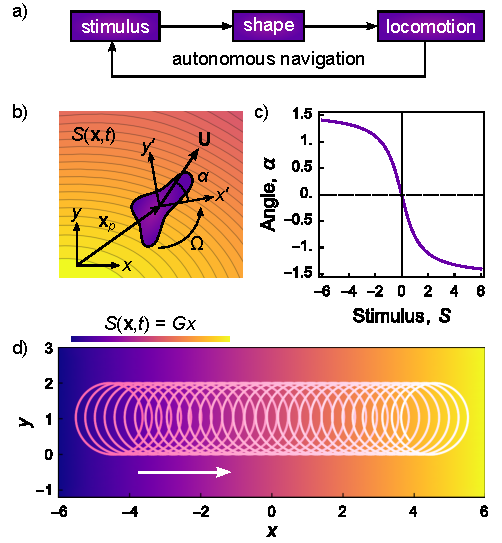
\includegraphics{figures/4_1.pdf}
     \caption{
     (a) A local stimulus determines particle shape which in turn directs particle motion towards new regions of the stimulus landscape.
     (b) An active particle moves with linear velocity $\ve{U}= U\cos\alpha \ve{e}_{x'} + U\sin\alpha \ve{e}_{y'}$ and angular velocity $\Omega\ve{e}_{z'}$ across a two-dimensional stimulus landscape $S(\ve{x},t)$.  
     (c) Assuming $R=U/\Omega=\text{constant}$, particle trajectories are determined by the stimulus-dependent orientation of the propulsion velocity $\alpha(S)$. Here, the function $\alpha(S)$ encodes for positive chemotaxis---that is, autonomous motion toward regions of higher stimulus. 
     (d) Computed trajectory of the particle in (c) on a uniform stimulus gradient $S(\ve{x})=G x$ of magnitude $G=0.1$. Here, lengths are scaled by the curvature radius $R$.}
     \label{fig:4.1}
 \end{figure}
%%%%%%%%%%%%%%%%%%%%%%%%%%%%%%


%%%%%%%%%%%%%%%%%%%%%%%%%%%%%%
\section{Self-phoretic Clusters}  
In practice, the design of the response functions $U(S)$, $\alpha(S)$, and $\Omega(S)$ requires one to consider the specific mechanism(s) of particle propulsion and its dependence on particle shape. Here, we consider the self-phoretic propulsion of hard sphere clusters, which have been studied previously in theory \autocite{soto2014self, varma2018clustering} and experiment \autocite{niu2018dynamics, schmidt2019light}. Each sphere $j$ in the cluster emits a constant flux $A_j$ of some chemical species, which sets up a concentration field $c(\ve{x})$ around the composite particle. At small P\'eclet number ($\text{Pe}=UL/D\ll1$), the species concentration is governed by the Laplace equation for steady-state diffusion, $\nabla^2c=0$, subject to the following boundary condition on the surface $\mathcal{S}_j$ of each sphere $j$
\begin{equation}
   -D\ve{n} \cdot \nabla c(\ve{x}) = A_j \quad \text{for} \quad \ve{x}\in \mathcal{S}_j
\end{equation}
where $D$ is the species diffusivity, and $\ve{n}$ is the unit normal directed out from the spheres.  Far from the particle, the species concentration approaches a constant value $c^{\infty}$, which can be set to zero without loss of generality. The resulting concentration field $c(\ve{x})$ depends on the shape of particle---that is, the configuration of its component spheres---but not its position and orientation within the stimulus landscape.

Concentration gradients tangent to the surface of each sphere drive interfacial phoretic flows with velocity 
\begin{equation}
    \ve{u}(\ve{x})=-\mu_j (\ve{\delta}-\ve{n}\ve{n}) \cdot \nabla c\quad \text{for} \quad \ve{x}\in \mathcal{S}_j
\end{equation}
where  $\mu_j$ is the mobility coefficient of sphere $j$.  At low Reynolds number ($\text{Re}=\rho UL/\eta$), the resulting velocity and pressure fields are governed by the Stokes equations, $-\nabla p + \eta \nabla^2 \ve{u}=0$ and $\nabla \cdot \ve{u}=0$, where $\eta$ is the fluid viscosity.  The linear velocity $\ve{U}$ and angular velocity $\ve{\Omega}$ of the rigid cluster is determined by the condition that there is no net force or torque on the particle.  We use a far-field approximation based on the method of reflections \autocite{varma2018clustering} to solve both the diffusion and hydrodynamic problems outlined above and estimate the particle velocity as a function of its shape \autocite{Supp}. For simplicity, we focus on the specific case of homogeneous clusters with $A_j=A$ and $\mu_j=\mu$; however, the model can also describe heterogeneous clusters made from spheres of different types.  We scale lengths by $L$, concentrations by $A L/D$, and velocities by $\mu A/D$, such that the velocities $\ve{U}$ and $\ve{\Omega}$ are determined entirely by particle geometry. \resp{Fig.\ \ref{fig:4.2}a shows the circular motion of an asymmetric three-sphere cluster as prescribed by the specific values of the sphere radii $a_i$ and the sphere-sphere separations $L_i$.}  

\section{Shape-shifting Clusters}  
In addition to shape-directed particle motion, we must also consider the effects of shape-shifting whereby the particle shape changes in response to changes in the local stimulus $S(\ve{x}_p,t)$.  Such particles can now be realized in experiment using stimuli responsive soft materials such as shape-changing polymers \autocite{magdanz2014stimuli} or liquid crystal elastomers \autocite{palagi2016structured} to alter the sizes and/or relative positions of spheres in the cluster.  In the present model, we consider a highly idealized form of shape-shifting, in which the bond lengths between neighboring spheres can depend on the local stimulus.  Fig.\ \ref{fig:4.2}b shows one example of a three-sphere cluster containing one stimuli-responsive bond.

%%%%%%%%%%%%%%%%%%%%%%%%%%%%%%
%%%%%%%%%%%%%%%%%%%%%%%%%%%%%%
\begin{figure}[!h]
    \centering
    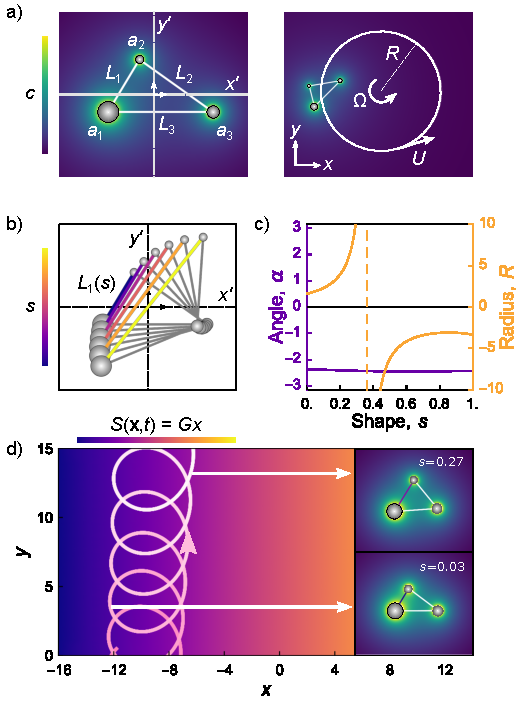
\includegraphics[width=8.5cm]{figures/4_2.pdf}
    \caption{Shape-shifting self-phoretic clusters. (a) Spheres connected by rigid bonds emit a chemical species that drives phoretic flows and particle motion with linear velocity $\ve{U}$ and angular velocity $\Omega$. Rigid particles move along circular trajectories of (signed) radius $R=U/\Omega$ (right). 
    (b) Standard shapes for different values of the shape parameter $s=(L_1-L_{\min})/(L_{\max}-L_{\min})$, which controls the length of one bond. The sphere positions $\ve{x}'_j(s)$ in the particle frame are chosen to eliminate particle translation and rotation due to shape change. 
    (c) Response functions $R(s)=U(s)/\Omega(s)$ and $\alpha(s)$ for the standard shapes in (b). 
    (d) Computed particle trajectory on a uniform stimulus gradient $S(\ve{x})=Gx$ of magnitude $G=0.2$; the shape parameter is assume to vary with the local stimulus as $s = (1+ e^{-S})^{-1}$. 
    In (a-d), the sphere radii are $a_1=0.1$, $a_2=0.04$, $a_3=0.06$; the fixed bond lengths are $L_2=0.860$ and $L_3=1$; the length of the responsive bond $L_1$ varies from $L_{\min}=0.5$ to $L_{\max}=1.5$.}
     \label{fig:4.2}
 \end{figure}
%%%%%%%%%%%%%%%%%%%%%%%%%%%%%%

To describe the motion of shape-shifting particles, we define a set of standard shapes that specify the position $\ve{x}_j'(s)$ of each sphere in the particle frame as a function of the shape parameter $s$ \autocite{shapere1989geometry}.  The standard shapes are chosen such that the particle frame does not translate or rotate within the viscous fluid as the particle changes its shape \autocite{Supp}.  In this way, we effectively remove the effects of particle swimming due to shape change, allowing us to focus exclusively on shape-induced changes in the propulsion velocity.  

For each standard shape, we compute the linear velocity $\ve{U}$ and angular velocity $\ve{\Omega}$ of the cluster as described above to obtain the response functions $U(s)$, $\alpha(s)$, and $\Omega(s)$. Fig.\ \ref{fig:4.2}c shows the response functions for a triangular cluster as a function of its one stimuli-responsive bond length, $s = (L_1 - L_{\min})/(L_{\max}-L_{\min})$.  This particle exhibits drifting motions in a stimulus gradient, but not the desired chemotactic motions parallel to the gradient direction (\resp{Fig.\ \ref{fig:4.2}d}).  In general, clusters will not satisfy the design criterion for chemotaxis that $R=\text{constant}$; however, it is possible to optimize their response by modifying the particle geometry.

\section{Design of Chemotactic Clusters} In designing chemotactic clusters that navigate up (or down) stimulus gradients, we seek to alter the cluster geometry such that each of the standard shapes leads to self-phoretic motion with a constant (signed) radius $R_0$. The design process can be formulated as an optimization problem that seeks to minimize the objective
\begin{equation}
    O(\ve{d}) = \langle [R(s,\ve{d})-R_0]^2 \rangle_s
\end{equation}
Here, the cluster geometry is parameterized by both the shape parameter $s\in[0,1]$ and the design variable $\ve{d}$, which is held fixed during shape-shifting.  The angle brackets denote averages over the shape parameter $s$, and $R(s,\ve{d})$ is the computed radius of the particle trajectory.

For the three-sphere cluster in Fig.\ \ref{fig:4.2}a, the design variable $\ve{d}$ includes two of the three radii ($a_2,a_3$) and one of the three bond lengths ($L_2$). All lengths are scaled by the length of the third bond $L_3$ such that $L_3\rightarrow 1$; the sphere radius $a_1$ is specified such that $a_1\ll L$ \resp{as required by the approximate model of phoretic propulsion outlined above}. The length $L_1$ of the stimulus-responsive bond is constrained to vary between user-specified limits $L_{\min}$ and $L_{\max}$. For each design $\ve{d}$, we compute the radius $R(s,\ve{d})$ of the particle trajectory as a function of the shape parameter using the model.  Numerical optimization methods can then be applied to identify the optimal shape-shifting particle.

Fig.\ \ref{fig:4.3}a highlights the performance of three different optimization methods based on hill climbing, random search, and the covariance matrix adaptation evolution strategy (CMA-ES) \autocite{hansen2016cma}, as applied to the design of chemotactic three-sphere clusters.  Greedy search algorithms such as hill climbing are quickly trapped in local minima; random searches are more effective but fail to identify the deepest minima.  The CMA-ES algorithm, which has proven effective on other problems involving colloidal clusters \autocite{miskin2013adapting}, combines stochastic ``mutation'' events with a deterministic ``selection'' process to identify optimal cluster geometries.  Fig.\ \ref{fig:4.3}b shows the optimal design for a three-sphere cluster with one stimuli-responsive bond.  Variations in the radius $R$ are ca.\ 2\% of the prescribed value (Fig.\ \ref{fig:4.3}c).  The orientation of the propulsion velocity $\alpha(s)$ decreases almost linearly with the shape parameter $s$ over a range spanning ca.\ 60$^{\circ}$. Assuming a sigmoidal response of the shape parameter on the local stimulus, the designed particle moves steadily up an applied stimulus gradient (positive chemotaxis; Fig.\ \ref{fig:4.3}d).

%%%%%%%%%%%%%%%%%%%%%%%%%%%%%%
\begin{figure}[!h]
    \centering
    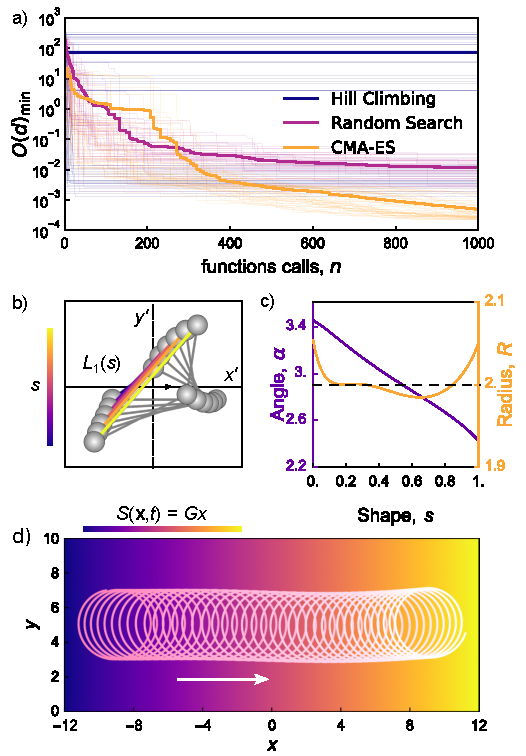
\includegraphics[width=8.5cm]{figures/4_3.pdf}
    \caption{Design of a chemotactic three-sphere cluster. (a) Minimum objective function $O(\ve{d})$ identified after $n$ function evaluations for three optimization methods initialized from 50 randomly selected designs (light curves); bold curves show the average performance. (b) Standard shapes for the optimal design for different values of the shape parameter $s=(L_1-L_{\min})/(L_{\max}-L_{\min})\in [0,1]$. During optimization, we prescribe the lengths $L_3=1$, $L_{\min}=0.5$, $L_{\max}=1.5$, $a_1=0.1$, and $R_0=2$; the optimal design identified is $a_2=0.0985$, $a_3=0.0958$, and $L_2=0.677$. (c) Computed response functions $\alpha(s)$ and $R(s)=U(s)/\Omega(s)$ for the standard shapes in (b). (d) Computed particle trajectory on a uniform stimulus gradient $S(\ve{x})=Gx$ of magnitude $G=0.2$; the shape parameter is assume to vary with the local stimulus as $s = (1+ e^{-S})^{-1}$.}
    \label{fig:4.3}
\end{figure}
%%%%%%%%%%%%%%%%%%%%%%%%%%%%%%

For spheres with the same activity and mobility connected by the same type of stimuli responsive bonds, one can design other particle clusters that behave in the opposite manner and swim down an applied gradient \autocite{Supp}.  Moreover, by altering the objective function, one can design particle clusters that navigate perpendicular to the gradient in a specified direction \autocite{Supp}. In addition to shape-shifting bonds between rigid spheres, one can also use responsive spheres that swell or shrink in response to local conditions. More generally, the present navigation strategy can be applied whenever particle motion depends on the local stimulus magnitude. Particle shape provides one of several possible design strategies for mediating this relationship between stimulus and motion.

\section{Effects of Noise} 
The type of autonomous navigation described here is only effective when rotational diffusion is slower than self-phoretic particle rotation.  Accounting for the particle's Brownian motion, the drift velocity in a uniform stimulus gradient $S(\ve{x},t)=G x$ can be approximated as $\ve{V}=-\tfrac{1}{2} G U R \alpha' \text{Pe}^2_r / (1+ \text{Pe}_r^2) \ve{e}_x +\mathcal{O}(G^2)$, where $\text{Pe}_r =\Omega\xi_r/k_B T$ is a rotational P\'eclet number, $\xi_r$ is a rotational friction coefficient (e.g., $\xi_r=8\pi\eta a^3$ for a sphere in an unbounded fluid), and $k_B T$ is the thermal energy.  As detailed in \autocite{Supp}, the derivation of this expression assumes that both the linear and angular propulsion velocity are independent of the stimulus (i.e., $U(S)=U$ and $\Omega(S)=\Omega$) and that the angular response function $\alpha(S)$ is approximately linear over changes in stimulus of order $GR$.  

For large P\'eclet numbers ($\text{Pe}_r\gg1$), the particle maintains orientational correlations over the duration of each circular orbit and uses this information to guide its motion on the stimulus landscape.  By contrast, rotational diffusion at small P\'eclet numbers ($\text{Pe}_r\ll1$) acts to erase these correlations thereby prohibiting effective navigation. Approximating the particle as a thin disk of diameter $L$ (such that $\xi_r=\tfrac{4}{3}\eta L^3$ \autocite{Kim2005}), the minimum particle size required for effective navigation ($\text{Pe}_r\sim1$) is $L\sim(3k_B T/4\Omega\eta)^{1/3}$.  Assuming a typical phoretic velocity of $\Omega=1$ rad/s, autonomous navigation in water ($\eta=10^{-3}$ Pa s) at room temperature requires particles sizes of order $L\sim 1~\mu$m or larger. Perhaps not surprisingly, this length is comparable to that of chemotactic bacteria such as \emph{E. coli}. \resp{Fig.\ \ref{fig:4.4} shows the  simulated  particle  motions  on  non-uniform gradients in the presence of Brownian motion.}

%%%%%%%%%%%%%%%%%%%%%%%%%%%%%%
\begin{figure}[h!]
     \centering
     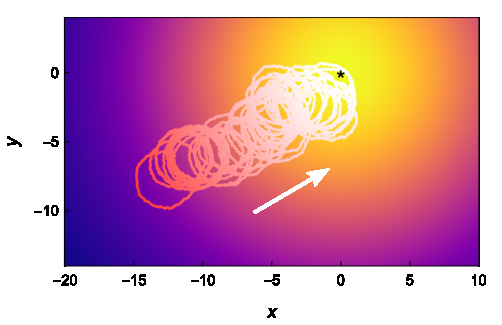
\includegraphics[width=8cm]{figures/4_4.pdf}
     \caption{\resp{Computed trajectory of the shape-shifting particle in Fig. \ref{fig:4.3}b-d moving on a peaked stimulus landscape with thermal noise. The stimulus is a Gaussian peak of width $\sigma=10$ and gradient magnitude $G=0.2$ centered at the origin, $S(x,y)= \sigma G  e^{-(x^2+y^2)/2\sigma^2}$; the  P\'eclet number is $Pe_r = 1000$.}}
     \label{fig:4.4}
 \end{figure}
%%%%%%%%%%%%%%%%%%%%%%%%%%%%%%

\section{Conclusions}  In sum, the shape-directed dynamics of shape-shifting particles provides a viable strategy for designing active colloids capable of autonomous navigation through heterogeneous environments.  While the present model focuses on self-phoretic motion, similar strategies should apply to other propulsion mechanisms that depend on particle shape (e.g., those based on external electric \autocite{Ma2015} or magnetic \autocite{Driscoll2017} fields).  The design of desired responses requires predictive understanding of both the relationship between stimulus and shape as well as the relationship  between shape and motion.  This design problem is simplest when the processes of shape-shifting and of shape-directed motion are effectively decoupled (e.g., when the former is much faster than the latter as assumed here). 

Recent advances in combining active colloids and stimuli-responsive materials should provide a promising platform to apply the design principles outlined here \autocite{Alvarez2019}. \resp{One significant challenge, however, is the often slow response times of existing shape-changing materials, which may be slower than that of particle propulsion (e.g., $\Omega^{-1}\sim 1$ s for phoretic propulsion). Experimental efforts to realize the proposed navigation strategy should therefore focus on shape-changing materials with fast response times such as some liquid crystal elastomers (LCEs) \autocite{camacho2004fast}.  Material deformations based on stimuli-dependent phase transitions should enable particles to navigate even small stimulus variations $\delta S$ about the transition $S_l$ where $\delta S \sim S_s \ll S_l$.  By incorporating material sensors and actuators, shape-shifting clusters can navigate autonomously on stimulus landscapes without the use of gradient-driven torques to bias their motion.} Looking forward, autonomous navigation based on internal degrees of freedom could be combined with external control strategies \autocite{liebchen2019optimal} to create colloidal robots capable of increasingly intelligent functional behaviors.

%\paragraph{\ydnote{Experimental realization guide }}
%\ydnote{Here we provide some basic guides to experimentally realize our proposed  shape-shifting autonomous navigation models. First, the choices of self-propulsion mechanism are not limited to the autophoretic particles. Any actuation mechanism(such as induced charge electrophoresis\autocite{brooks2018shape}, light induced thermophoresis\autocite{lozano2016phototaxis}, acoustic actuation\autocite{sabrina2018shape},  catalytic  self-electrophoresis\autocite{brooks2019shape})  for active colloids can be considered based on the materials of particles. Second,the candidates for shape-shifting materials including shape memory polymers/hydrogel \autocite{kirillova2019shape}, shape memory alloys \autocite{rodrigue2017overview}, liquid crystal elastomer\autocite{palagi2016structured} or composite materials\autocite{hu2018small}, etc. Shape-shifting materials can be the joints between active particles or active particles themselves.  The microstuctured particles can be farbricated with MEMS tech or chemical synthesis\autocite{leong2009tetherless}. One thing need to emphasized here that actuation source should be different from the shape-shifting source. For example, the particles can be light responsive shape-shifting driven by induced charge electrophoresis. Third, a physics model such as the autophoretic clusters model in this paper should be built to express relations between particles' shape and velocity.In the partical experiment model, an relaxation time $\tau_{relaxation}$ can be added to represent the reponse speed of the material to the stimulus. Shape of particles and shape-shifting path then can be designed following this paper's strategy to achieve the desired autonomous navigation behaviors.}






%%%%%%%%%%%%%%%%
% Chapter 5
%%%%%%%%%%%%%%%%
\chapter{Autonomous navigation of micro-magnetic rollers} \footnotetext{This chapter is adapted from Dou, Yong, and Kyle JM Bishop. "Autonomous navigation of shape-shifting microswimmers." Physical Review Research 1.3 (2019): 032030.}
\section{Introduction}
\section{Experiment}
\section{Discussion}
\section{Conclusion}

%%%%%%%%%%%%%%%%

%%%%%%%%%%%%%%%%
% Chapter 6
%%%%%%%%%%%%%%%%

\chapter{Colloidal robots: the end of the beginning }
\begin{center}
\textbf{Abstract}
\end{center}
This thesis started with introducing the motivation and background of colloidal robot. A fully autonomous colloidal robot should have a feedback system composed of actuators, sensors, and controllers.  In Chapter 2 and Chapter 3, we gave two examples on how to make actuators for colloidal robots with a high efficient electrostatics actuation mechanism called contact charge electrophoresis (CCEP). Chapter 2 showed the asymmetry of the colloid particle can provide a large design space for different kinds of actuation motions in colloidal robots.  Chapter 3 showed complex traveling actuation for colloidal robots can be achieved by coupling individual actuator's motion together.  In addition to actuation, we further proposed two strategies to design sensors and controllers for colloidal robots. With actively interacting the with environment through the feedback system, colloidal robots can finish some complex targets such as autonomous navigation. In Chapter 4, colloidal robots are designed to alter the shape versus the local information or stimulus. We programmed the shape and shape-shifting process versus different stimuli to let colloidal robots achieve global navigation with only local information. In Chapter 5, we programmed the external magnetic field used to actuate ferromagnetic colloidal robots. Such colloidal robots were also demonstrated to show navigation behaviors  (uphill or downhill) on an inclined slope. Though we have showed inspiring achievement with both experiment and computation efforts in this thesis, research pathway towards colloidal robot is just at the end of the beginning (or even not reach). Lots of more interesting and challenging problems still need to be solved related to colloidal robots field. The last chapter of this thesis is going to give an outlook for the future research direction of colloidal robots.
\section{Actuation Mechanism for  Colloids Robots}
 Lots of current actuation mechanisms have either very low energy conversion ($<0.1\%$) efficiency due to a large amount of heat dissipation or very slow speed, which is not compatible to the real living machines such as bacteria. Future development for  the actuation mechanism should focus on improving efficiency, speed, and robustness as well as understanding the detailed physics behind different mechanisms. Moreover, colloidal robots introduced in this thesis and lots of other papers have very limited degrees of freedom for their motions. Such motions are usually simply rolling, translating or turning around which is far from the various actuation mode in a robotic hand with many joints. New actuation mechanisms should also let colloidal robots have more degrees of freedom to move.  Another important characteristics of a good actuation mechanism  is flexible and robust. The actuation mechanism should work reliably for a large range of materials in different fluid environments. With respect to the robust characteristic,  the magnetic actuation mechanism stands out from other mechanisms. Because the magnetic force can be well controlled with less influences from the fluid environments or materials (as the example shown in chapter 5).

One interesting electrostatics actuation mechanism called Quincke rotation, which can generate fast autonomous rotation near the electrode with very low energy input is a promising new actuation mechanism \autocite{das2013electrohydrodynamic}. Different shapes such as spheres, ellipsoids and helix have shown high actuation speed in microscale\autocite{brosseau2019relating,das2019active}. A better understanding of dynamics in Quincke rotation can help us design faster and more efficient colloidal robots. However, the complex non-linear multipole electrodynamics and hydrodynamics problems in Quincke rotation are still unsolved, requiring  both experimental and theoretical study. More accurate  and  less time-consuming algorithm should be developed\autocite{fiore2019fast}.

Another research direction is developing a well packed autonomous platform to drive the motion of colloid  robots.  The autonomous platform should integrate the process in colloidal robots research from fabrication, observation to analysis and recycling. In an autonomous process, the platform can produce colloidal robots and insert colloidal robots into the experimental environment autonomously. Then the imaging process will be triggered  with feedback loop to actuate the microrobots. After observation, the colloidal robots should be collected by the platform for future implementations. A similar autonomous platform has been built to study chemical synthesis and biology research \autocite{grizou2020curious,chao2019systems}. The autonomous workflow platform can not only saving time during research but also accelerates the commercialized process of colloidal robots.   

\section{Swarm Colloidal Robots}
Swarm colloidal robots take advantage of the interactions among colloidal particles to generate high-level functions such as pattern formation and collective behaviors. In Chapter 3, we showed linear colloidal particle actuators can form travelling waves. An intuitive research direction is to explore 2 dimension electrostatic actuators' dynamics with the same system in Chapter 3. For the experiment, we can use two parallel plate electrodes and place actuators between the electrodes in a honeycomb or square lattice  holes to study the dynamics. The dynamics structures in 2D will be much more visually impressive than  1-d travelling waves. However,  there are some experimental technique challenges to put micron particles  inside micro honeycomb lattice holes. One possible solution is to use laser tweezers to place the micro particles into each hole one by one. Alternatively, we can also MEMS 's top-down fabrication to make the micro spheres in the micro holes with multiplayer's lithography, deposition, and etching. To model the system, it is very important to find a suitable coarse-grain model instead of direct detailed numerical simulations of all the particles. The coarse-grain model should be simple enough that doesn't require too much computational source, while it should be accurate enough to capture the key physics and  behaviors in the system similar to the model proposed in Chapter 3.

As we discussed in the first chapter, most of the swarm colloidal robots now are simply using passive interaction showing only one type of dynamics, which is not programmable. If the interactions between the colloidal particles can be re-programmed, a different mode of collective behaviors could be generated. Recent research has shown that the magnetic interactions between magnetic particles   can be programmed by introducing multi-pole interactions. These magnetic particles were programmed to show  different  equilibrium self-assembly structures subject to different interactions\autocite{niu2019magnetic}. Similar programmed method can be used in non-equilibrium swarm colloidal robots to generate different dynamics patterns. Moreover, collective behaviors among large amounts of micro scale colloidal particles  will generate impact in macro scale,  showing reconfigurable, adaptable and scalable  characteristics,  which is similar to  how the small living cells built the whole body. Thus, swarm colloidal robots can even provide revolutionary new actuation mechanism for the real size robotics. 
%%%%%%%%%
\section{Shape Shifting Colloids Robots}
To experimentally realize the autonomous navigation strategy with shape-shifting colloidal robots in Chapter 4, the key is to develop shape-shifting materials responding to the environmental stimulus. There several candidate materials such as  light response liquid crystal\autocite{palagi2016structured}, and thermal response shape memory alloy\autocite{busch1991shape}: liquid crystal can change the molecule's structure upon receiving photons from  light, leading to the shape shifting of liquid crystal; the atom lattice of shape memory alloy will change due to the thermal energy and will release back to normal in the room temperature. These materials have been reported working very well in microscale to form different structure subject stimulus\autocite{breger2015self}, although most papers use shape-shifting as a mechanism to actuate instead of sensing\autocite{tu2017self,li2018light}. A possible experiment system could use a dielectric (or magnetic nanoparticle embedded) light response liquid crystal materials with some designed shape.   The motion can be actuated via the outside electrostatic (or magnetic) field. With different environmental stimuli, the materials will change to different shapes simultaneously. The colloidal robots will continue the feedback loop of sensing and actuation, leading to navigation behaviors shown in Chapter 4. 

There several challenges to be solved for the experiment proposed above. The first challenge  is to design the shape shifting process for colloidal robots. We gave a simple example in Chapter 4 on how to design the shape-shifting process with the reverse design optimization. However, it will be hard to build a model perfectly predicting the motions of all different shape colloids in external field. Numerical models need to work together with large experiments efforts to help us fully understand how shape can direct different motions for colloidal robots\autocite{lee2019directed}. Then with a "dictionary" of shape and its corresponding motion, we can try to design the shape shifting process for colloidal robots based on the guideline in Chapter 4. The second challenge is to match the time scale between shape shifting rate and actuation speed. The changing rate of current shape shifting materials is relatively very low that will take seconds or even minutes to change one shape to another. When the colloidal robots sense a new environmental stimulus, it should change the shape simultaneously without too  much time delay. Late reaction time (or called as long memory) of shape-shifting materials will  lead to the wrong navigation direction of colloidal robots. Future research should focus on developing materials with fast-changing rate. The third challenge is to built a microscale stimulus landscape. The gradient of stimulus landscape should be small enough compared to the size of colloidal robots that colloidal robots only feel a uniform stimulus in one location. This requires a very precise  design of the micron scale topological structure such as micro patterned light grid to control the light intensity. 

Moreover, shape-shifting materials are working as only sensors. So if other internal states can change with the stimulus from the environments, these states can also be used as sensors for colloidal robots. For example, if the electric charge amount, some chemical species, the strength of magnetic dipole on the colloidal robots can change versus the environmental stimulus, all of these quantity can be used as sensors in a feedback loop to design the autonomous navigation strategy for colloidal robots.




\section{Programmable and Design the Colloids Robots}
For engineering applications and commercialized requirements, colloidal robots must be programmed and designed rationally, which is still a relatively blank research area. This is because most researchers in colloidal robots are from natural science fields like chemistry and physics. It is a pity that colloidal robots haven't arisen too much attention from researchers in robotics such as electrical engineers or computer scientists, who focus more on the programming and design problems\autocite{das2019cellular}.  The control strategy, design framework and program algorithm in large scale robots can help a lot in the research on colloidal robots.  Future research on colloidal robots should involve intensive collaborations between robotics field and colloid fields.

One very promising  direction is to use machine learning or artificial intelligent guiding the design of colloidal robots. There are lots of design parameters for a colloidal robot such as materials choice, shape's design, magnitude and form of the power source. The typical way for experimentalists is to do tons of repeating experiments either successful approaches or failed attempts during the research. The machine learning approach can make failure data more valuable. With clustering, classification and regression for the experimental data, machine learning (or deep learning) algorithm can not only find the pattern to design a good colloidal robot, but also be likely to find some nontrivial design rules for colloidal robots. In addition to studying large amounts of data with machine learning, optimization algorithm (or optimal design) can help us design colloidal robots with less time-consuming experiment approaches. If we know the design space for the colloidal robots, either with the experimental or simulation output, optimization algorithms (such as CME-ES algorithm in Chapter 4 can guide the selection of next design parameters in the design space. Also, recent reports showed Bayesian inference can help to estimate design parameters with fewer experiments \autocite{winslow2019characterization}.



Also, there are more functions beyond autonomous motion and navigation could be designed for colloidal robots. Cargo transportation is now an emerging research direction\autocite{demirors2018active,Martinez-Pedrero2015}. Basically, the colloidal robots can use physical interactions in the form of electrostatic, magnetic to hydrodynamics to attract and capture cargo. The colloidal robots will move cargo along some designed route and release the cargo in the destination via turning the interaction off. Future research could focus  on the developing method for cargo sorting and cargo assembling similar to Amazon robots in macro scale.


\section{Application of Colloidal Robots}
At the current stage, all of the colloidal robots' applications are still being explored in the lab. But with the unique properties of colloidal robots (cell scale size and different dynamics function), the potential applications for colloidal robots are very impressive. In the last section of this thesis, I will briefly discuss the applications for colloidal robots.

\textbf{Biomedical applications.} The biggest and most intuitive applications for the colloidal robots are medical applications. Colloidal robots are usually in the size of living cells so that they may work as "micro" surgery knives to remove tumors, transport drug or repair wound for patience. Several in vivo colloidal robotic experiments  on animals have been reported with promising results\autocite{Gao2015,li2018development}. There are several very strict standard must be satisfied when we design a colloidal robot for biomedical applications. First, the materials of colloidal robots must be biocompatible with no harm to the living system and have a pathway to be removed from the living body or alternatively can be digested by the living body without any side effects. The materials should also be modified to have proper chemical or physical affinity so that colloidal robots can carry drugs or attack the tumors in the living system. Some candidate materials are silica gel materials (PDMS) or some nontoxic metals. This requires tremendous in vivo experiments on animals before  any possible experiments on the human being. Second, the actuation mechanism for the colloidal robots must also be safe enough. For example, if we use a magnetic or electric field, the intensity of the external field shouldn't exceed the maximum bearing value of humans. These fields also shouldn't be  filtered or screened by some structures inside the human body. Therefore, magnetic field or acoustic field that have already by used in medical treatment are good  candidate actuation mechanisms.  Third, the cost of the whole colloidal robot's system should be kept as affordable as possible so that colloidal robots are tangible for most patients. Research on colloidal robots for biomedical applications must involve collaborations from doctors and scientists in medical school to get their insights and knowledge.

\textbf{Other applications.} Colloidal robots have been demonstrated with other interesting applications such as cleaning water, mixing fluid and lithography\autocite{soler2014catalytic,fei2019magneto,li2014nanomotor}. These applications all depend on the autonomous motion and navigation of colloidal robots. As a chemical engineer, I would like to propose an interesting application in the chemical engineering field: colloidal robots may be a new technology to enhanced oil recovery from the ground. In the petroleum industry, a large amount of crude oil (more than 50$\%$) is not extracted from rocks because they are in some dead-end micro pores with very low Reynolds number. colloidal robots with autonomous motion and navigation behaviors can be designed with good crude oil affinity via chemical/physical modification. Then we can send these colloidal robots into the micro pore full of oil.  Then colloidal robots  can collect the oil in micro poles and be navigated back with the crude oil.

As a short summary, colloidal robots seem to be something from science fiction, but it is really happening now with many scientists and engineers from different fields working on it. We have some basics theoretical frameworks and some simple experimental demonstrations. The author has a very optimistic expectation for the future fast development of colloidal robots. Maybe in five or ten years, colloidal robots can be commercialized and serve people in different areas.  



%%%%%%%%%%%%%%%%

%%%%%%%%%%%%%%%%

% Conclusion
%%%%%%%%%%%%%%%%


%
\begin{center}
\pagebreak
\vspace*{5\baselineskip}
\textbf{\large Conclusion }
\end{center}


\begin{flushleft}
\hspace{10mm}Use this page for your epilogue or conclusion if applicable; please use only one of the titles for this page. Otherwise, you may delete it.
\end{flushleft}


%\pagenumbering{gobble}  %remove page number on summary page



%addcontentsline{toc}{chapter}{Conclusion and Outlook}


%%%%%%%%%%%%%%%%
% References
%%%%%%%%%%%%%%%%

\titleformat{\chapter}[display]
{\normalfont\bfseries\filcenter}{}{0pt}{\large\bfseries\filcenter{#1}}  % Reset title format for Reference section. (It is different from Chapter titles)
\titlespacing*{\chapter}
  {0pt}{0pt}{30pt}




\begin{singlespace}  % use single-line spacing for multi-line text within a single reference
	\setlength\bibitemsep{\baselineskip}  %manually set separataion betwen items in bibliography to double space
	\printbibliography[title={References}]
\end{singlespace}









\addcontentsline{toc}{chapter}{References}  %add References section to Table of Contents

%%%%%%%%%%%%%%%%
% Appendices
%%%%%%%%%%%%%%%%

%Readjust Title format for Appendicies
\titleformat{\chapter}[display]
{\normalfont\bfseries\filcenter}{}{0pt}{\large\chaptertitlename\ \large\thechapter : \large\bfseries\filcenter{#1}}  
\titlespacing*{\chapter}
  {0pt}{0pt}{30pt}	%controls vertical margins on title
  
% Adjust section title formatting
\titleformat{\section}{\normalfont\bfseries}{\thesection}{1em}{#1}

% Adjust subsection title formatting
\titleformat{\subsection}{\normalfont}{\thesubsection}{0em}{\hspace{1em}#1}

\begin{appendices}

%Some Table of Contents entry formatting
\addtocontents{toc}{\protect\renewcommand{\protect\cftchappresnum}{\appendixname\space}}
\addtocontents{toc}{\protect\renewcommand{\protect\cftchapnumwidth}{6em}}

%Begin individual appendices, separated as chapters

\chapter{Supporting Information for Chapter 2}
This appendix compares the experimental results between pure dielectric particles and  Janus particles undergoing CCEP. The results demonstrate the partial charge on the dielectric semi sphere of Janus Particle, which may explain the variation in the particles’ lateral displacement during oscillation. The theoretical details of electrostatics and low Reynolds number hydrodynamics are also shown to support out plausible mechanism of directed motion in Chapter 2.  


\section{\new{Additional Experiments and Estimates}}


%%%%%%%%%%%%%%%%%%%%%%%%%%%%%%
%%%%%%%%%%%%%%%%%%%%%%%%%%%%%%
\subsection{\new{CCEP Dynamics of Dielectric (non-Janus) Particles}} \label{sec:Dielectric}

As a control experiment, we examined the behavior of bare silica particles ($8~\mu\text{m}$ diameter) in mineral oil when subject to an applied electric field.
Surprisingly, these insulating particles also oscillated between the two electrodes but at much lower frequencies than the metal-coated particles.
For an applied voltage $V=800~\text{V}$ and electrode separation $H=200~\mu\text{m}$, silica particles oscillated with a average frequency of ${\sim}0.1~\text{Hz}$ as compared to ${\sim}100~\text{Hz}$ for similar metallodielectric Janus particles (Fig.~\ref{fig:Silica}a). 
Dielectric particles spent most of their time at the electrode surface before rapidly moving off towards the opposite electrode.
We examined the characteristic time $\tau$ required for a particle near the electrode surface to leave the focal plane of the microscope (Fig.~\ref{fig:Silica}a,b).
This time was of order $\tau\sim 5~\text{ms}$ for both Janus and dielectric particles, indicating that the different particles moved at similar velocities.
These observations suggest that Janus particles and dielectric particles acquire similar amounts of charge but at different rates.
Further study is required to better characterize and understand the charging of dielectric materials on contact with biased electrodes.

\begin{figure}[h]
    \centering
    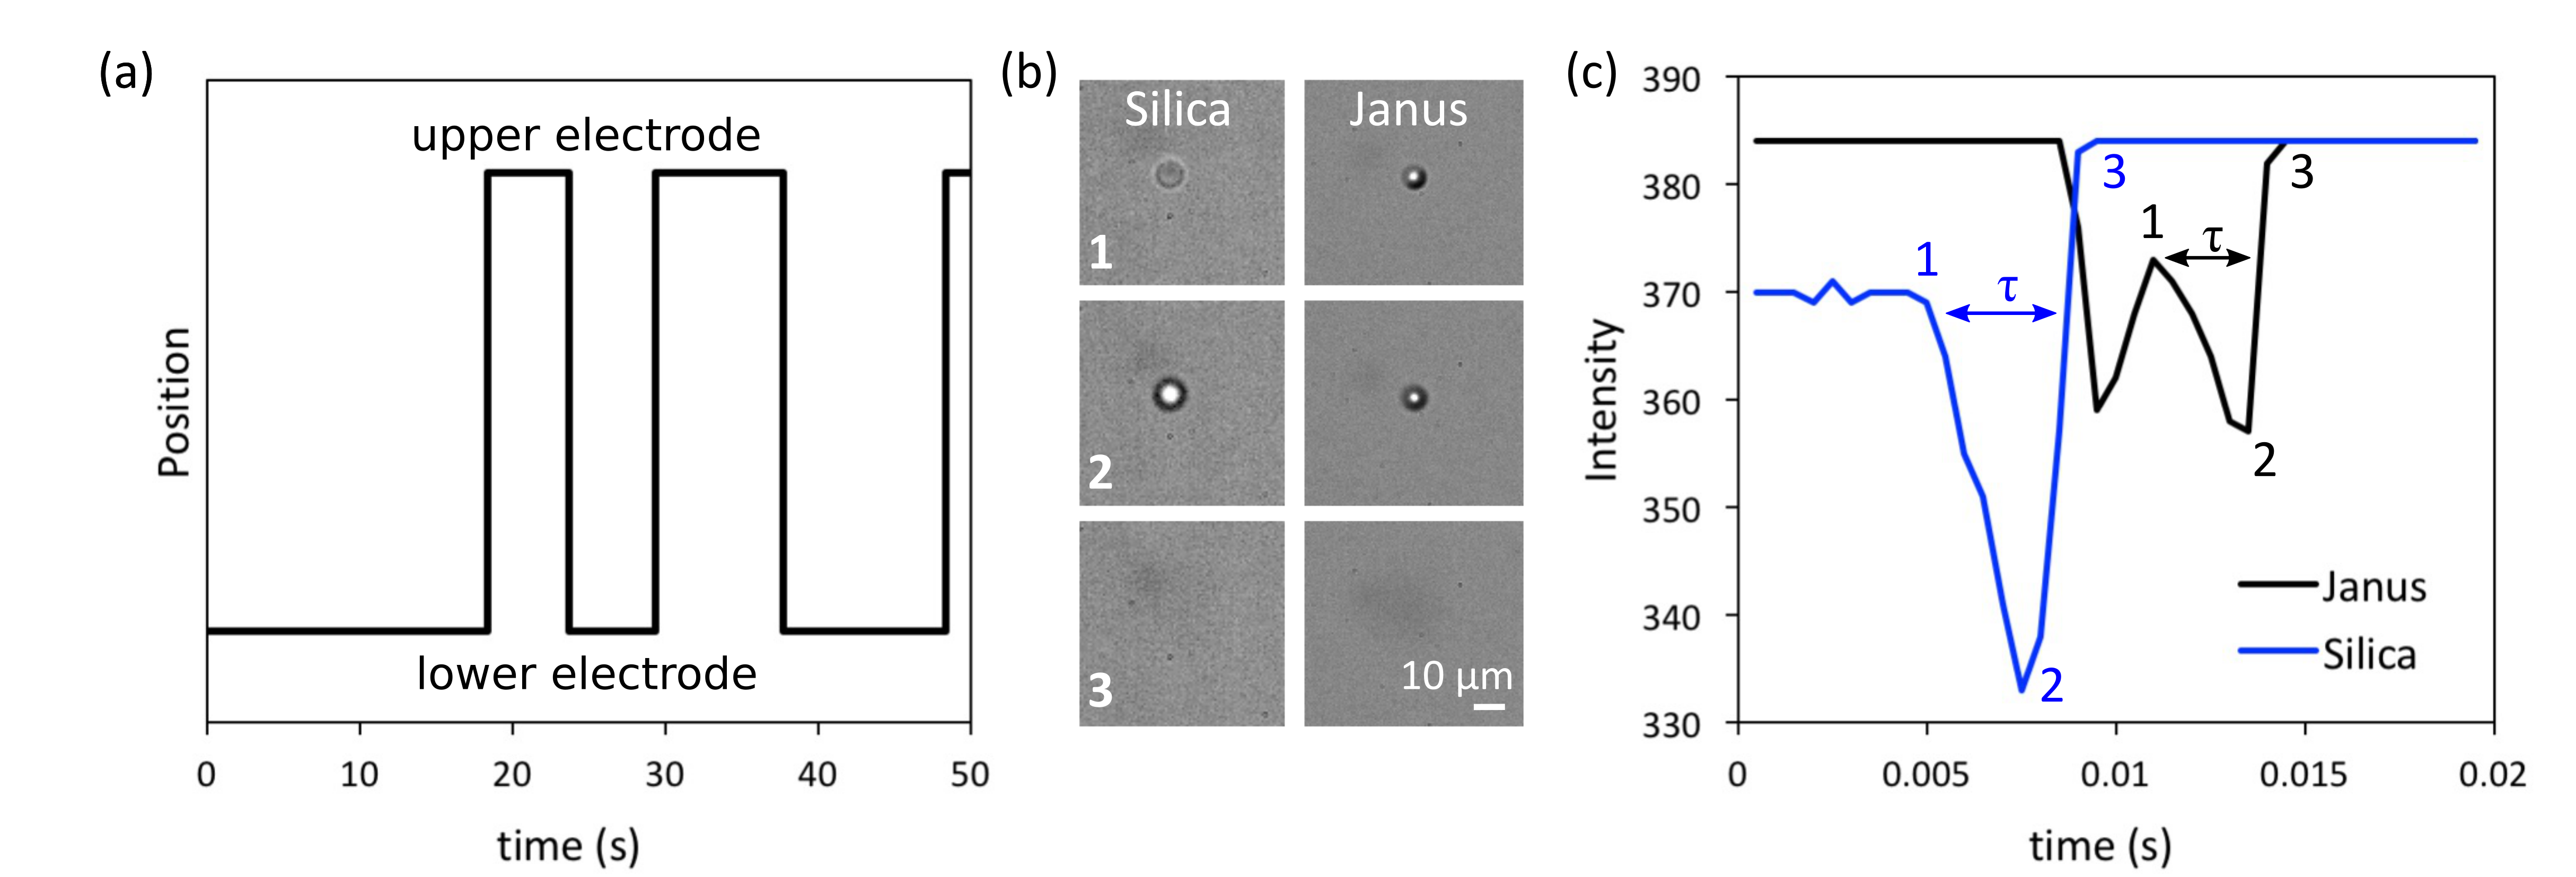
\includegraphics[width=\textwidth]{figures/A1_SilicaParticles.png}
    \caption{(a) A single silica particle oscillates between two parallel electrodes ($V=800~\text{V}$, $H=200~\mu\text{m}$). (b) Microscopy images show a silica particle (left) and a Janus particle (right) near the lower electrode as they move out of focus; the different particles leave the electrode surface at similar rates. (c) The average intensity vs.~time for the image series in (b). The characteristic time $\tau$ required for the particle to move out of focus is indicated for each particle.}
    \label{fig:Silica}
\end{figure}


%%%%%%%%%%%%%%%%%%%%%%%%%%%%%%
%%%%%%%%%%%%%%%%%%%%%%%%%%%%%%
\subsection{\new{Variations in Janus Particle Dynamics}}

In experiment, we measured the lateral displacement $\Delta_i$ and the oscillation period $T_i=t_{i+1}-t_{i}$ for the $i^{\text{th}}$ oscillation of each particle.
These measured quantities show significant variations both from one oscillation to the next and from particle to particle. 
Here, we quantify these variations and discuss their likely origins.
Figure \ref{fig:Variations} shows the displacement and period for several different particles during 50 oscillation cycles.
For each particle, there was little or no correlation between the displacement and the period; the coefficient of determination averaged over 10 different particle was $\langle R^2\rangle=0.29$.
Similarly, the average displacement of each particle was not correlated to its average period ($R^2 = 0.22$).
These results suggests that variations in the displacement are largely independent from those in the period; these quantities can therefore be considered separately.
For each particle, we computed the standard deviation of displacement and the period for the 50 oscillation cycles.
For the displacement, the standard deviation ranged from $0.13~\mu\text{m}$ ($20\%$ of the mean) to $0.81~\mu\text{m}$ ($60\%$) with an average variation of $0.50~\mu\text{m}$ ($40\%$).
For the period, the standard deviation ranged from $2.0~\mu\text{s}$ ($8\%$ of the mean) to $9.7~\mu\text{s}$ ($28\%$) with an average variation of $4.8~\mu\text{s}$ ($15\%$).

\begin{figure}[h]
    \centering
    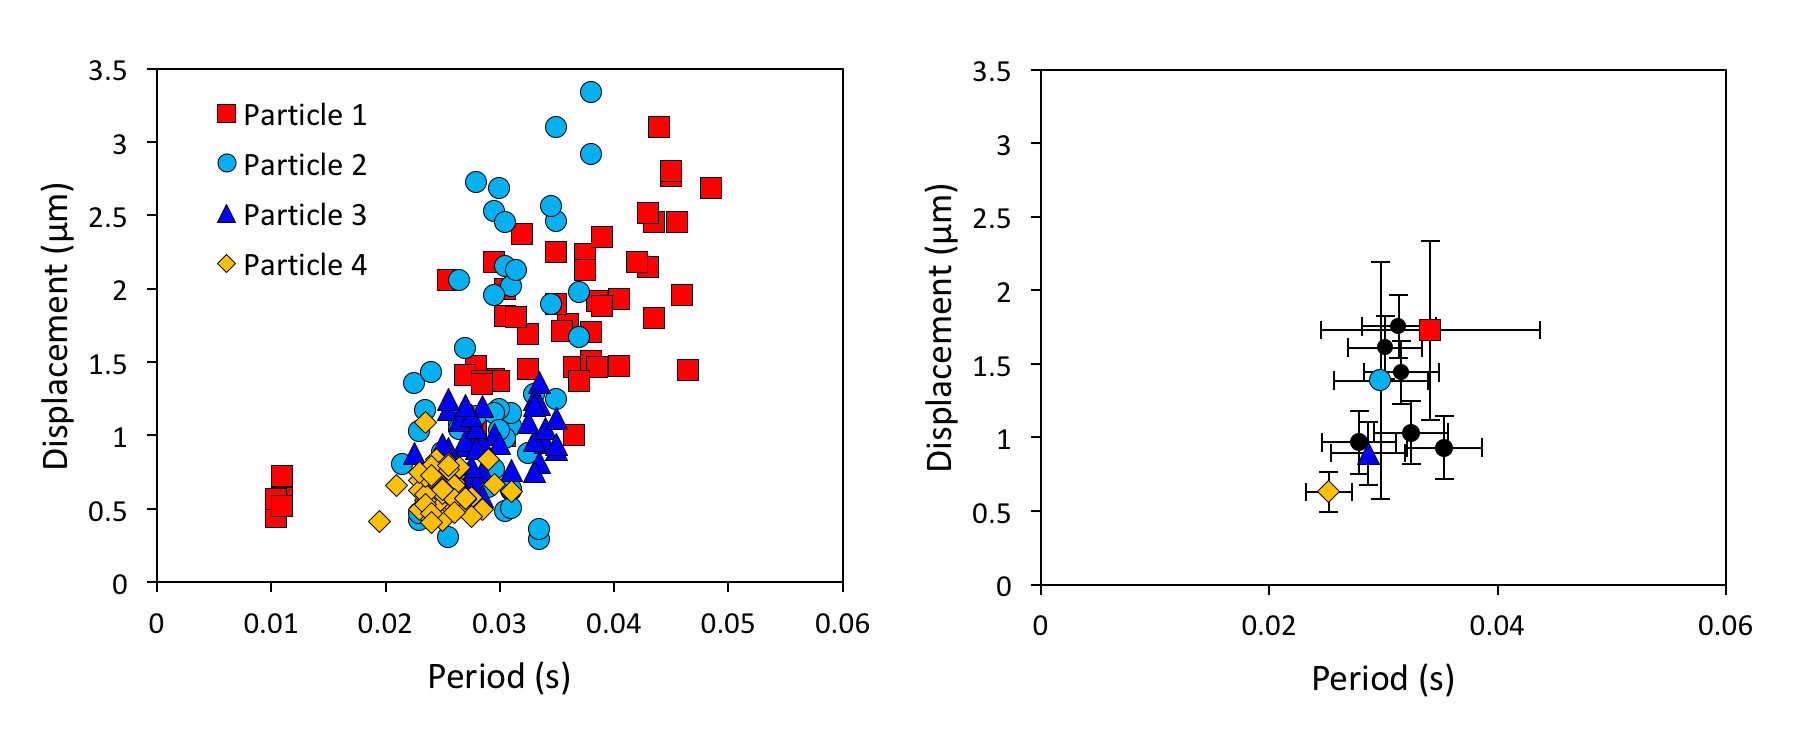
\includegraphics[width=\textwidth]{figures/A1_VariationPlots.png}
    \caption{(left) Lateral displacement $\Delta$ vs.~oscillation period $T$ for four particles showing 50 oscillation cycles. (right) Average displacement vs.~average period for 10 particles; error bars denote one standard devation above/below the mean. Here, the applied voltage is $V=800~\text{V}$ and the electrode separation is $H=200~\mu\text{m}$.}
    \label{fig:Variations}
\end{figure}

Variations in the oscillation period were likely due to differences in the the amount of charge acquired by the particle during electrical contact with the electrode \autocite{drews2015contact}.
The charging process is believed to proceed by an electric discharge, which occurs when the local electric field between the particle surface and the electrode exceeds some critical value.
Importantly, this discharge is extinguished before the particle can acquire its ``full'' equilibrium charge (\emph{i.e.}, that expected when the particle potential is equal to that of the electrode).
Variations in the duration of the discharge may cause variability in the amount of charge acquired by the particle.
The oscillation period is expected to depend inversely on the particle charge as $T\propto q^{-1}$.
By contrast, the lateral displacement is only weakly dependent on the charge (Fig.~\ref{fig:Displacement}).

There are several possible sources of variation in the particles' lateral displacement.
First, the resolution of the microscope images ($0.25~\mu\text{m per pixel}$) limits our ability to identify the location of the particle center with accuracy greater than ${\sim}0.25~\mu\text{m}$.
Second, the displacement depends on the separation $\delta$ between the particle and the electrode at electrical contact; this distance is likely variable owing to the stochastic nature of the electric discharge that mediates charge transfer.
Third, particle to particle variation may arise due to imperfections in the metallic hemisphere and/or charge on the dielectric hemisphere; these effects are thought to be responsible for the circular trajectories observed in experiment.

%%%%%%%%%%%%%%%%%%%%%%%%%%%%%%
%%%%%%%%%%%%%%%%%%%%%%%%%%%%%%
\subsection{\new{Native Charge on the Dielectric Hemisphere}}

In our analysis, we neglected effects due to native charge on the dielectric hemisphere of the Janus particle.
Here, we provide order-of-magnitude estimates to support this assumption.
We assume that the zeta potential $\zeta$ of a homogeneous dielectric sphere is on the order of the thermal potential $k_BT/e\sim25~\text{mV}$. 
Using the linear Poisson-Boltzmann equation \autocite{berg2014effects}, the zeta potential is related to the surface charge as $\sigma=\varepsilon(1+\kappa a)\zeta/a$, where $\kappa$ is the Debye screening length. 
For micron sized particles in mineral oil, the screening length is larger than particle (see estimate below) such that $\sigma\sim \zeta/a$. Alternatively, the charge density acquired by a conductive sphere upon contact with an electrode is $\sigma_c\sim \varepsilon E$. 
The native charge is therefore negligible when $Ea/\zeta \gg 1$; in the present experiments, this ratio is of order $10^3$.
As discussed above (Section \ref{sec:Dielectric}), significant amounts of charge may be present on the dielectric surface due to contact charging with the electrode.

The Debye screening length in mineral oil is estimated to be $\kappa^{-1}\sim 20~\mu\text{m}$ based on the definition $\kappa = (2e^2 n_0/\varepsilon k_B T)^{1/2}$ where $n_0\sim10^{15}~\text{ions/m}^3$ is the ion density. 
The ion density is estimated from the measured electrical conductivity of mineral oil as $K = e n_0 / \lambda\sim 10^{-12}~\text{S/m}$ where $e$ is the elementary charge, and $\lambda\sim6\pi\eta a_i$ is an approximate ion drag coefficient in mineral oil (viscosity, $\eta = 0.027~\text{Pa s}$; ion radius, $a_i = 0.2~\text{nm}$) \autocite{cartier2014microfluidic}.  


%%%%%%%%%%%%%%%%%%%%%%%%%%%%%%
%%%%%%%%%%%%%%%%%%%%%%%%%%%%%%
\subsection{\new{Electrothermal Effects}}

It is unlikely that electrothermal effects contribute significantly to the particle motions observed in experiment.
During contact charging, the flow of charge to/from the particle heats the fluid near the point of contact possibly inducing thermal flows. 
An order-of-magnitude estimate reveals the relevant temperature variations to be quite small.  
Charge of order $q\sim4\pi a^2 E$ is transferred to the particle over a characteristic voltage $aE$. 
The total energy dissipated by Joule heating is estimated as the product of these quantities, $4\pi a^3 E^2$, which is of order $4\times10^{-13}~\text{J}$ (assuming $a = 4~\mu\text{m}$, $E = 5~\text{V/}\mu\text{m}$).  
Equating the energy dissipated by Joule heating to the adiabatic heating of mineral oil in a volume comparable to the particle size yields a temperature increase of $T\sim4\pi a^3E^2/\rho c_p a^3\sim 10^{-3}~\text{K}$ (assuming density $\rho = 850~\text{kg/m}^3$ and specific heat $c_p = 1700~\text{J/kgK}$) for mineral oil).






%%%%%%%%%%%%%%%%%%%%%%%%%%%%%%
%%%%%%%%%%%%%%%%%%%%%%%%%%%%%%

\section{Theoretical Details}

%%%%%%%%%%%%%%%%%%%%%%%%%%%%%%
%%%%%%%%%%%%%%%%%%%%%%%%%%%%%%
\subsection{Electrostatics}

%%%%%%%%%%%%%%%%%%%%%%%%%%%%%%
\subsubsection{Charged Janus Particle in a Uniform Electric Field}
\label{sec:unbounded}

We consider a metallodielectric Janus sphere of radius $a$ positioned in an unbounded dielectric fluid and subject to a uniform electric field $\ve{E}^{\infty}$.
One half of the sphere is a perfect conductor; the other is a dielectric with permittivity $\varepsilon$ assumed equal to that of surrounding fluid. 
The conductive hemisphere has a constant charge $q$, which is acquired on electrical contact with an electrode surface (see below).
Let $\ve{b}$ be the unit vector directed from the center of the particle towards the pole on the conductive hemisphere.
The electric potential $\Phi$ within the dielectric fluid is governed by the Laplace equation
\begin{equation}
    \nabla^2\Phi = 0. \label{eq:laplace}
\end{equation}
Far from the particle, the potential is given by
\begin{equation}
    \Phi(\ve{r}) = \Phi^{\infty}(\ve{r}) = -\ve{r}\cdot\ve{E}^{\infty} \text{ for } r\rightarrow\infty,
\end{equation}
where $r=0$ at the center of the sphere.
The potential on the conductive hemisphere is a constant $\Phi(\ve{r})=\Phi_p$, such that the total charge satisfies 
\begin{equation}
    q = \int_{S_p} -\varepsilon \ve{n}\cdot\nabla\Phi dS,\label{eq:charge}
\end{equation}
where $\ve{n}$ is the unit normal vector directed outward from the surface of the conductive hemisphere $S_p$.

The above equations can be solved for the potential $\Phi$ and the electric field $\ve{E}=-\nabla\Phi$ surrounding the conductive hemisphere of the of the particle.
The net electric force on the Janus particle can then be computed by integrating the Maxwell stress over the conductive hemisphere as
\begin{equation}
    \ve{F} =  \int_{S_p} \frac{1}{2}\varepsilon E^2 \ve{n} dS = q \ve{E}^{\infty}.
\end{equation}
Similarly, the electric torque about the particle center can be computed as
\begin{equation}
    \ve{L} =  \int_{S_p} \frac{1}{2}\varepsilon E^2 (\ve{r}\times \ve{n}) dS = L \frac{\ve{b}\times\ve{E}^{\infty}}{|\ve{b}\times\ve{E}^{\infty}|}.
\end{equation}

Scaling lengths by $a$, the electric potential by $a E^{\infty}$, and charge by $q_s=4\pi\varepsilon a^2 E^{\infty}$, this electrostatic problem is fully characterized by two dimensionless quantities: (i) the orientation of the Janus sphere relative to the field as characterized by the angle $\alpha$ (where $\ve{b}\cdot\ve{E}^{\infty} = E^{\infty} \cos\alpha$), and (ii) the scaled charge on the particle $q / q_s$.
Furthermore, owing to the linearity of the Laplace equation, the torque on the particle is a linear function of the charge and may be expressed as
\begin{equation}
    L(\alpha,q) = \varepsilon a^3 {E^{\infty}}^2 \left[g_0^{\infty}(\alpha) + g_1^{\infty}(\alpha) \left(\frac{q}{q_s}\right) \right], \label{eq:torqueInf}
\end{equation}
where $g_0^{\infty}(\alpha)$ and $g_1^{\infty}(\alpha)$ are dimensionless functions. These functions were computed numerically using a commercial finite element solver (COMSOL) as illustrated in Figure \ref{fig:TorqueFunctions}.

\begin{figure}[h]
    \centering
    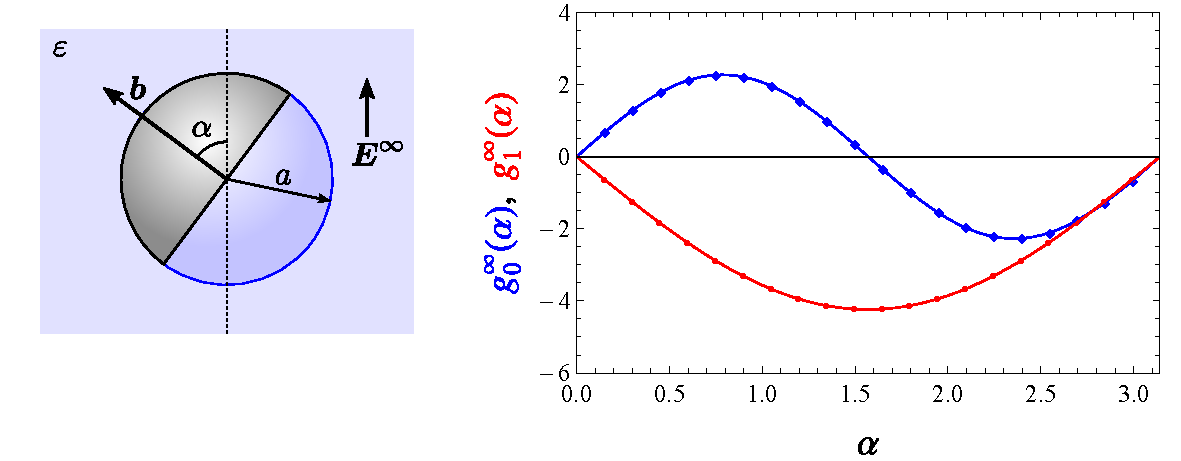
\includegraphics[height=5cm]{figures/A1_Unbounded.pdf}
    \caption{(\emph{left}) Schematic illustration of a Janus particle in a uniform electric field $\ve{E}^{\infty}$.  (\emph{right}) Dimensionless functions $g_0^{\infty}(\alpha)$ and $g_1^{\infty}(\alpha)$ used in equation (\ref{eq:torqueInf}) to compute the electric torque $L$ on a Janus sphere in an unbounded medium. The markers are computed using COMSOL; the solid curves are least squares fits of the form $g_0^{\infty}(\alpha)=A\sin(2\alpha)$ and $g_1^{\infty}(\alpha)=B \sin(\alpha)$ (with $A=2.27$ and $B=-4.24$).}
    \label{fig:TorqueFunctions}
\end{figure}


Depending on the magnitude of the charge $q$, the Janus sphere may adopt different stable orientations, for which $L(\alpha) = 0$ and $L'(\alpha) < 0$.  When the net charge on the particle is zero, the particle orients perpendicular to the applied field ($\alpha = \pi/2$). Conversely, when the particle charge is large such that $q\gg q_s$, the particle prefers to align parallel with the applied field ($\alpha \rightarrow 0$ for $q>0$ or $\alpha \rightarrow \pi$ for $q<0$). For intermediate charges (like those found in the experiment), the stable orientation of the particle lies between these limiting extremes -- namely, $0<\alpha<\pi/2$ for positively charged particles. Importantly, when the sign of the particle is reversed, it experiences an electric torque that rotates the particle into a newly stable orientation. It is this rotational motion in proximity to the electrode surface that results in the translational motion of the particle.


%%%%%%%%%%%%%%%%%%%%%%%%%%%%%%
\subsubsection{Contact-Charging of a Janus Particle at an Electrode Surface}

The charge acquired by a metallodielectric Janus sphere on contact with either of the coplanar electrodes can be estimated by assuming that charge flows onto / from the conductive hemisphere until its potential is equal to that of the proximal electrode.
Specifically, we consider the charging of a particle positioned at height $z_p = a + \delta$ above a planar electrode at $z=0$; here, $\delta$ is the surface separation, which is assumed small compared to the particle radius ($\delta\ll a$).
The potential on the electrode and the conductive hemisphere are assumed to be zero
\begin{equation}
    \Phi(\ve{r}) = 0 \text{ for } \ve{r} \in \text{electrode or particle}. \label{eq:nearBC}
\end{equation}
Far from the electrode, the potential approaches that due to the applied field $\ve{E}^{\infty}=E^{\infty}\ve{e}_z$
\begin{equation}
    \Phi(\ve{r}) = -z E^{\infty} \text{ for } \ve{z} \rightarrow \infty. \label{eq:farBC}
\end{equation}
Solving the Laplace equation (\ref{eq:laplace}) subject to boundary conditions (\ref{eq:nearBC}) and (\ref{eq:farBC}), the charge $q$ on the particle is then computed using equation (\ref{eq:charge}).
For a fixed surface separation $\delta$, the charge acquired on contact depends only on the orientation of the particle relative to the surface as illustrated in Figure \ref{fig:ContactCharge}.

\begin{figure}[h]
    \centering
    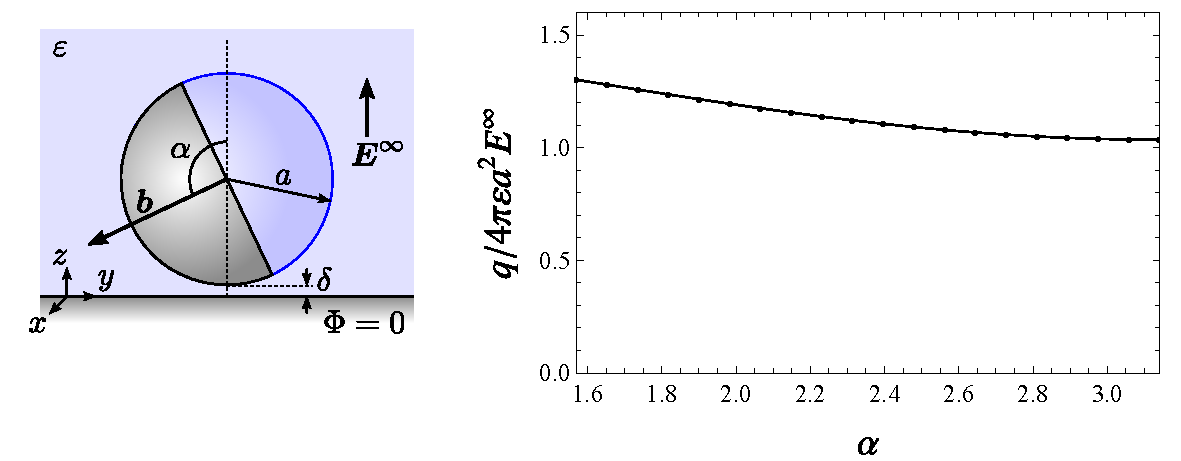
\includegraphics[height=5.5cm]{figures/A1_ContactCharge.pdf}
    \caption{(\emph{left}) Schematic illustration of a Janus particle in electrical contact with a planar electrode. (\emph{right}) Charge acquired by the particle (scaled by $4\pi \varepsilon a^2 E^{\infty}$) as a function of its orientation.  Here, the surface separation is $\delta= 0.02 a$ (similar results are obtained for other $\delta$ provide $\delta\ll a$). The plot markers are computed using COMSOL; the solid curve is a least squares fit of the form $y=A + B \cos x$ (with $A=1.30$ and $B=0.266$).}
    \label{fig:ContactCharge}
\end{figure}


%%%%%%%%%%%%%%%%%%%%%%%%%%%%%%
\subsubsection{Electric Force and Torque on a Janus Particle at Finite Surface Separations}

In section \ref{sec:unbounded}, we evaluated the force and torque on a Janus particle in an unbounded medium subject to a uniform electric field.  We now consider the case when the surface of the particle is separated by a dimensionless distance $\xi=(z_p-a) / a$ from a grounded plane.  The force and torque on the particle depends on the particle orientation $\alpha$, on the surface separation $\xi$, and the particle charge $q$ as
\begin{gather}
    F(\alpha,h,q) = \varepsilon a^2 {E^{\infty}}^2 \left[f_0(\alpha,\xi) + f_1(\alpha,\xi) \left(\frac{q}{q_s}\right)  + f_2(\alpha,\xi)\left(\frac{q}{q_s}\right)^2 \right], \label{eq:Force}
    \\
    L(\alpha,h,q) = \varepsilon a^3 {E^{\infty}}^2 \left[g_0(\alpha,\xi) + g_1(\alpha,\xi) \left(\frac{q}{q_s}\right)  + g_2(\alpha,\xi)\left(\frac{q}{q_s}\right)^2 \right].\label{eq:Torque}
\end{gather}
Here, the dimensionless functions $f_i(\alpha,\xi)$ and $g_i(\alpha,\xi)$ were computed numerically and approximated by parametric interpolants of the form
\begin{gather}
    f_i(\alpha,\xi) = \sum_{j=0}^{15}\sum_{k=0}^5 A_{ijk} \frac{\cos j\alpha}{\xi^k},\label{eq:ForceInterpolant}
    \\
    g_i(\alpha,\xi) = \sum_{j=1}^{15}\sum_{k=0}^5 B_{ijk} \frac{\sin j\alpha}{\xi^k},\label{eq:TorqueInterpolant}
\end{gather}
where the coefficients $A_{ijk}$ and $B_{ijk}$ are determined by linear least squares regression (Figure \ref{fig:ForceTorque}). In the limit of large surface separations ($h\rightarrow\infty$), the solution approaches the result described in the previous section 
\begin{gather}
    f_0(\alpha,h)\rightarrow0,~~ f_1(\alpha,h)\rightarrow4\pi,~~ f_2(\alpha,h)\rightarrow0,
    \\
    g_0(\alpha,h)\rightarrow g_0^{\infty}(\alpha),~~ g_1(\alpha,h)\rightarrow g_1^{\infty}(\alpha),~~ g_2(\alpha,h)\rightarrow0.
\end{gather}
Knowledge of the force and torque is necessary to describe the translational and rotational dynamics of a Janus particle as it approaches an electrode, reverses charge, and returns towards the opposite electrode.

\begin{figure}
    \centering
    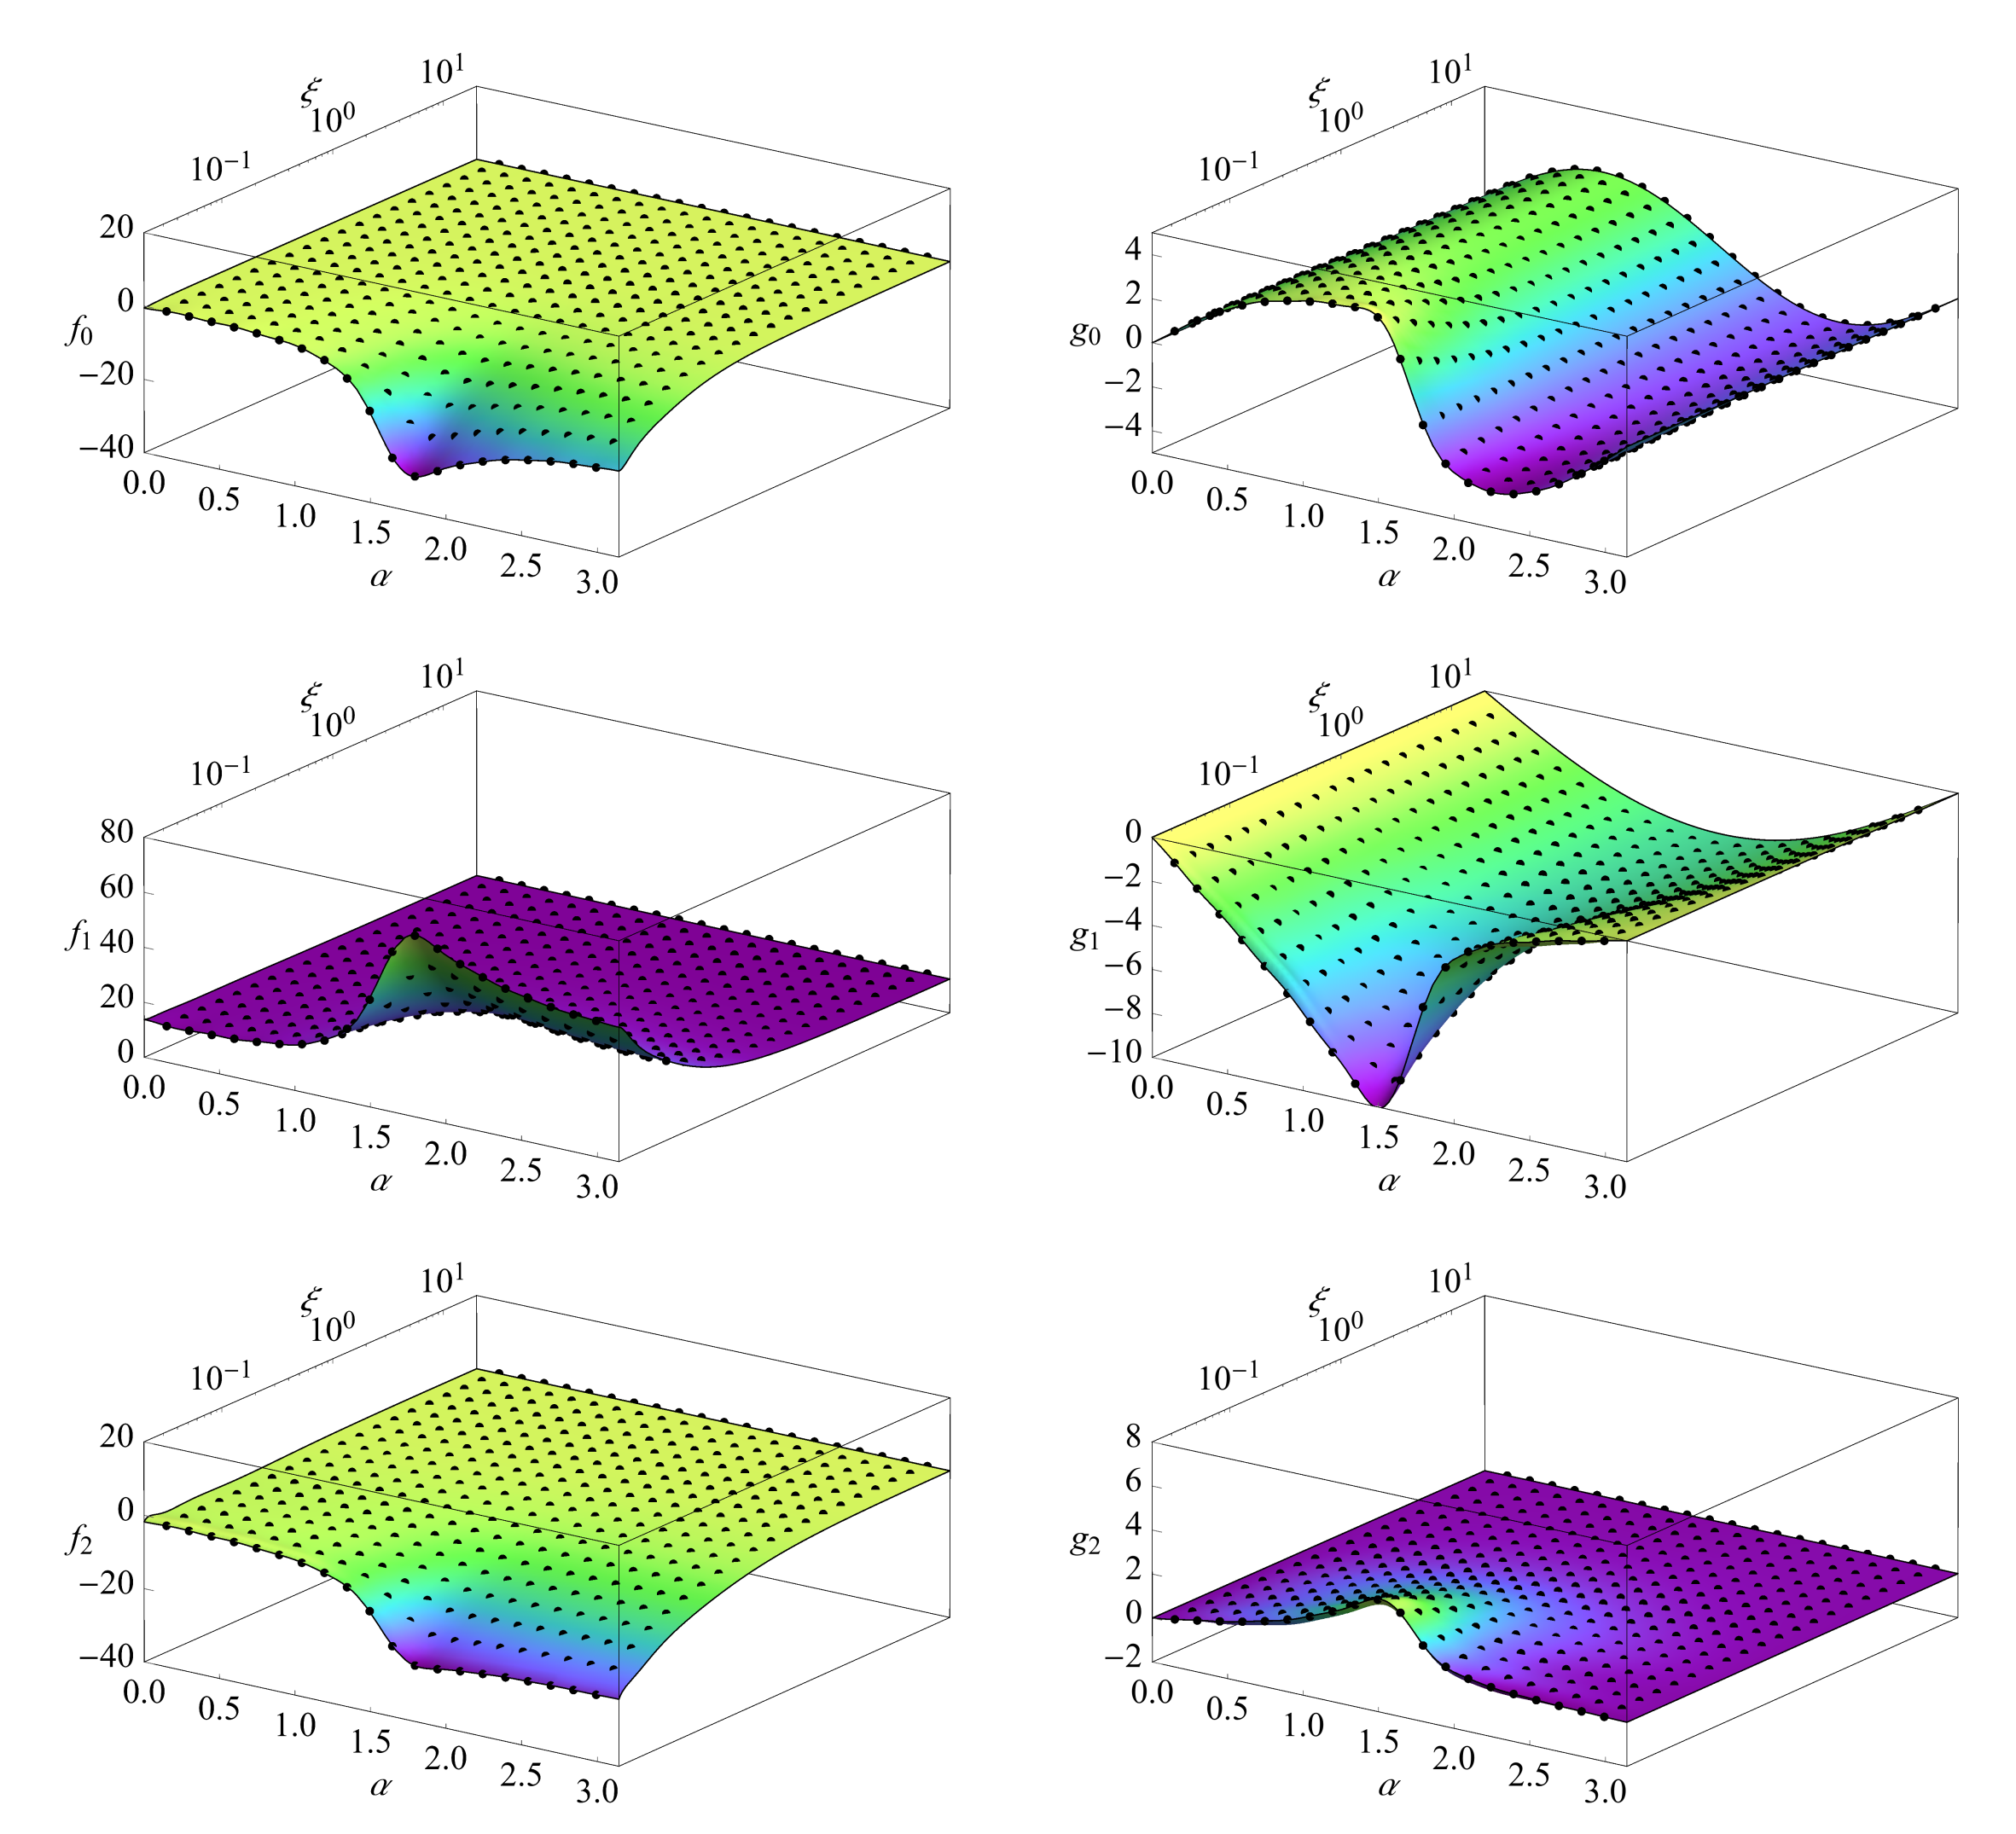
\includegraphics[width=15cm]{figures/A1_ForceTorque.png}
    \caption{Dimensionless functions $f_i(\alpha,\xi)$ and $g_i(\alpha,\xi)$ used in equations (\ref{eq:Force}) and (\ref{eq:Torque}) to evaluate the force and torque on a charged Janus particle near a grounded plane. The parameter $\alpha$ describes the orientation of the particle; $\xi=(zp-a)/a$ describes its separation from the surface. The markers are computed numerically using COMSOL; the surfaces are least squares interpolants given by equations (\ref{eq:ForceInterpolant}) and (\ref{eq:TorqueInterpolant}).}
    \label{fig:ForceTorque}
\end{figure}


%%%%%%%%%%%%%%%%%%%%%%%%%%%%%%
%%%%%%%%%%%%%%%%%%%%%%%%%%%%%%
\subsection{Hydrodynamics}

At low Reynolds numbers, the electric force $\ve{F}$ and torque $\ve{L}$ acting on the particle gives rise to its translational and rotation motion as described by the linear relation
\begin{equation}
    \begin{bmatrix}
    \ve{F} \\ \ve{L}
    \end{bmatrix}
    =
    \begin{bmatrix}
    \ve{A} & \tilde{\ve{B}}
    \\ 
    \ve{B} & \ve{C}
    \end{bmatrix}
    \cdot
    \begin{bmatrix}
    \ve{U} \\ \ve{\Omega}
    \end{bmatrix}, \label{eq:resistance}
\end{equation}
where $\ve{U}$ and $\ve{\Omega}$ are the translation and rotational velocities of the particle, and  $\ve{A}$, $\ve{B}$, $\tilde{\ve{B}}$, and $\ve{C}$ are hydrodynamic resistance tensors.  For a spherical particle moving near a solid plane ($z=0$), the components of the resistance tensors take the form 
\begin{gather}
    A_{ij} = 6\pi\eta a \left[ X^A \delta_{i3}\delta_{j3} + Y^A (\delta_{ij} - \delta_{i3}\delta_{j3}) \right], 
    \\
    B_{ij} = \tilde{B}_{ji} = 6\pi\eta a^2 \left[ Y^B \varepsilon_{3ij} \right],
    \\
    C_{ij} = 6\pi\eta a^3 \left[  X^C \delta_{i3}\delta_{j3} + Y^C (\delta_{ij} - \delta_{i3}\delta_{j3}) \right], 
\end{gather}
where $\delta_{ij}$ is the Kronecker delta, and $\varepsilon_{ijk}$ is the permutation symbol. The coefficients $Y^A$ and $Y^B$ describe, respectively, the dimensionless force and torque on a sphere translating \emph{parallel} to a solid plane surface \autocite{ONeill1964a}. The coefficient $Y^C$ describes the torque on a sphere rotating about an axis \emph{parallel} to the surface \autocite{Dean1963}. The coefficient $X^A$ describes the force on a sphere translating \emph{perpendicular} to the surface \autocite{Brenner1961a}.  Finally, $X^C$ describes the torque on a sphere rotating about an axis \emph{perpendicular} to a the surface \autocite{Jeffrey1915}. These coefficients depend only on the dimensionless surface separation $\xi = (z_p - a)/a$ as illustrated in Figure \ref{fig:resistance}. 

\begin{figure}[h]
    \centering
    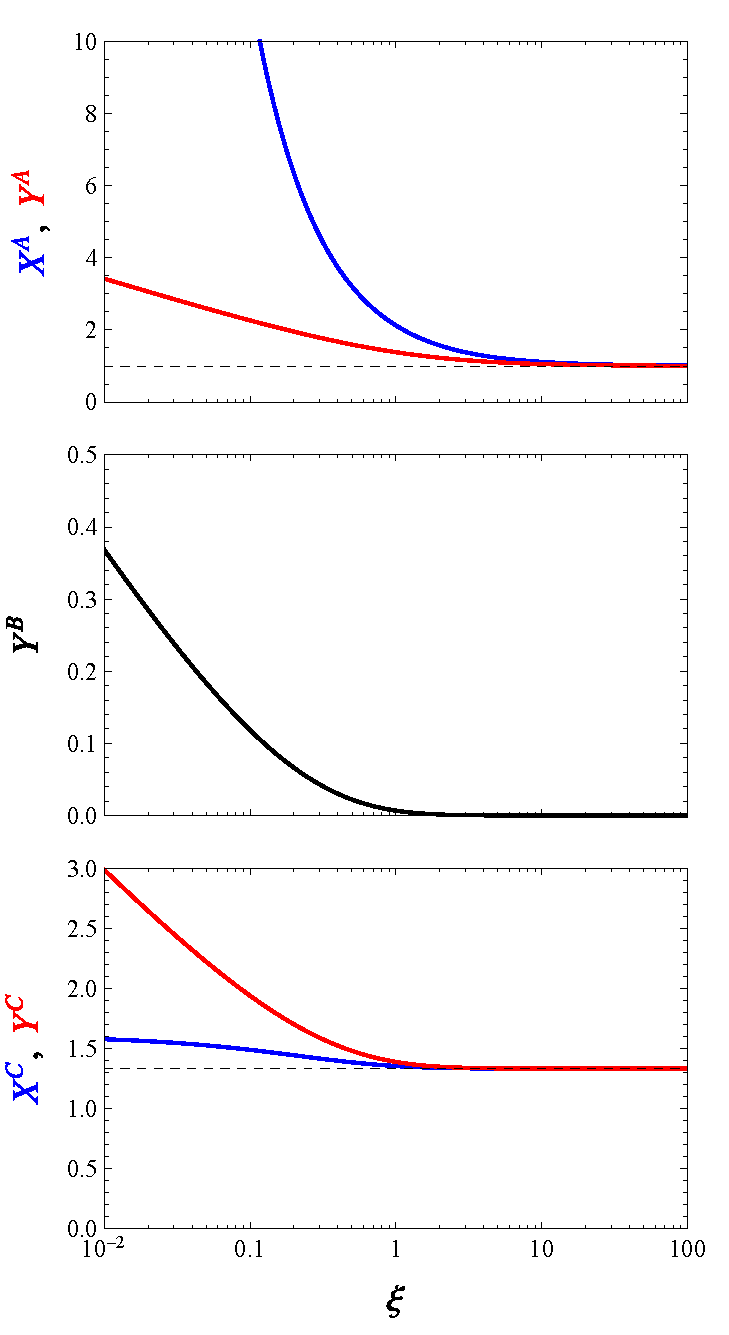
\includegraphics[width=7cm]{figures/A1_resistance.pdf}
    \caption{Resistance coefficients for a sphere of radius $a$ as a function of the surface separation $\xi=(z_p-a)/a$ with plane surface at $z=0$. The dashed lines denote the behavior of an isolated particle in an unbounded medium.}
    \label{fig:resistance}
\end{figure}

%%%%%%%%%%%%%%%%%%%%%%%%%%%%%%
%%%%%%%%%%%%%%%%%%%%%%%%%%%%%%
\subsection{Particle Dynamics}

We now consider the dynamics of a single Janus particle as it approaches the plane electrode at $z=0$, makes electrical contact, and then moves off towards the opposite electrode. We assume that the particle director $\ve{b}$ lies in the $yz$ plane throughout the ``collision'' (Figure \ref{fig:Collision}).  For this geometry, symmetry implies that $F_x=F_y=L_y=L_z=0$, and equation (\ref{eq:resistance}) can be inverted to obtain
\begin{align}
    U_y &= \dot{y}_p =- \frac{1}{6\pi\eta a^2} \left(\frac{Y^B L_x}{Y^A Y^C - {Y^B}^2}\right),
    \\
    U_z &= \dot{z}_p = \frac{1}{6\pi\eta a} \left( \frac{F_z}{X^A}\right),
    \\
    \Omega_x &= \dot{\alpha} = \frac{1}{6\pi\eta a^3} \left(\frac{Y^A L_x}{Y^A Y^C - {Y^B}^2} \right).
\end{align}
Here, resistance coefficients depend on the dimensionless separation $\xi$ between the particle and the surface; the force and torque depend on both the surface separation $\xi$ and the angle $\alpha$. These dynamical equations can be integrated numerically to describe the translational and rotational motion of the particle in time. 

Figure \ref{fig:Collision} illustrates the dynamics of two such particle ``collision'' with the electrode surface. Initially, the particle is negatively charged.  It moves towards the surface with a fixed orientation until reaching a finite surface separation $\delta$, at which point its charge reverses sign. Upon the change in polarity, the particle  rotates towards its new stable orientation.  The rotation of the particle in close proximity to the plane surface results in a net displacement $\Delta$ away from the conductive hemisphere of the particle.  Note that the magnitude of this displacement depends on the particle charge $q$ and the surface separation $\delta$ at contact (Figure \ref{fig:Displacement}).

\begin{figure}[h]
    \centering
    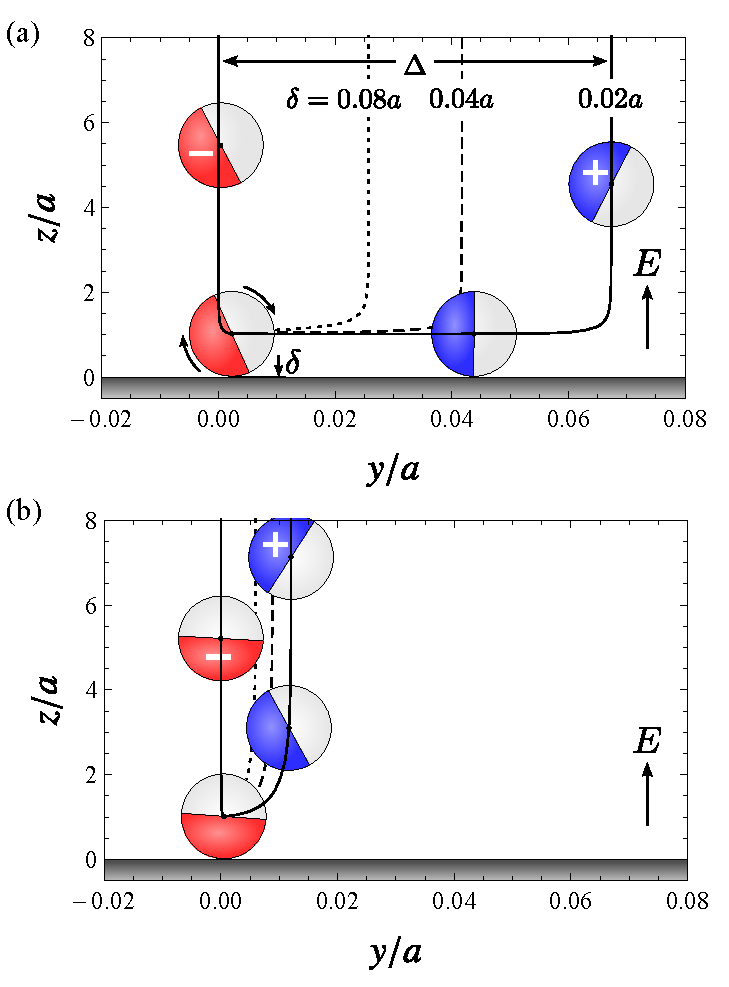
\includegraphics[width=9cm]{figures/A1_Collision.pdf}
    \caption{ Simulated particle ``collisions'' with the lower electrode for a particle charge (a) $q=\pm0.5q_s$ and (b) $q=\pm1.058q_s$. The solid curve shows the trajectory of the particle center; the orientation of the particle at different points along the trajectory is illustrated graphically. The net particle displacement $\Delta$ depends on the surface separation $\delta$ at ``contact'' when the particle charge reverses polarity. Note that for clarity the $z$ and $y$ axes use different scales.}
    \label{fig:Collision}
\end{figure}

\begin{figure}[h]
    \centering
    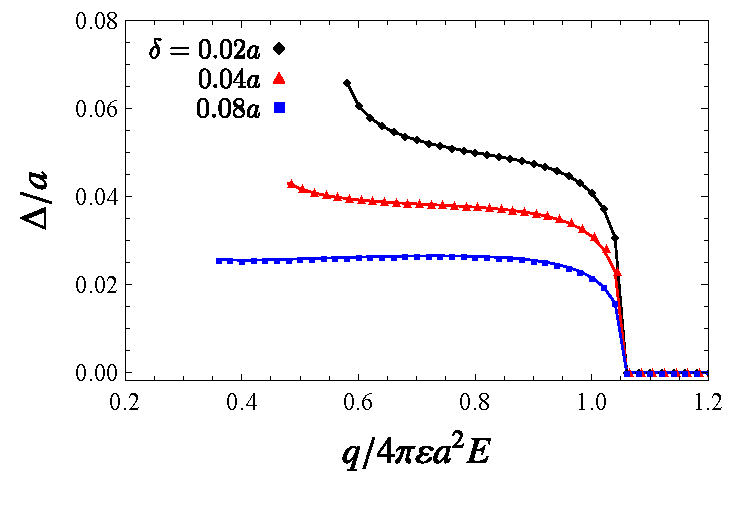
\includegraphics[width=9cm]{figures/A1_Displacement.pdf}
    \caption{Net displacement $\Delta$ of a Janus particle during a single particle ``collision`` as a function of the particle charge $q$ for three different contact separations $\delta$. Note that when the charge acquired is below some critical value (open circles), the particle remains bound to the electrode \autocite{drews2015contact}.}
    \label{fig:Displacement}
\end{figure}




%%%%%%%%%%%%%%%%%%%%%%%%%%%%%%
%%%%%%%%%%%%%%%%%%%%%%%%%%%%%%




\end{appendices}
\begin{appendices}

%Some Table of Contents entry formatting
\addtocontents{toc}{\protect\renewcommand{\protect\cftchappresnum}{\appendixname\space}}
\addtocontents{toc}{\protect\renewcommand{\protect\cftchapnumwidth}{6em}}

%Begin individual appendices, separated as chapters

\chapter{Supporting Information for chapter 3}

In this appendix, several additional experimental results are shown to characterize the formation and dynamics of travelling waves in Chapter 4. The breaking frequency and maximum wavelength are depend on the number of actuators. We also perform additional simulations of a more detailed model to assess the importance  of  amplitude  dynamics.  These simulations  reveal  that  the  approximate  model  based  on  weakly-coupled  phase  oscillators performs well for the experimental conditions.

%%%%%%%%%%%%%%%%%%%%%%%%%%%%%%%%%%%%
\begin{figure}[p]
    \centering
    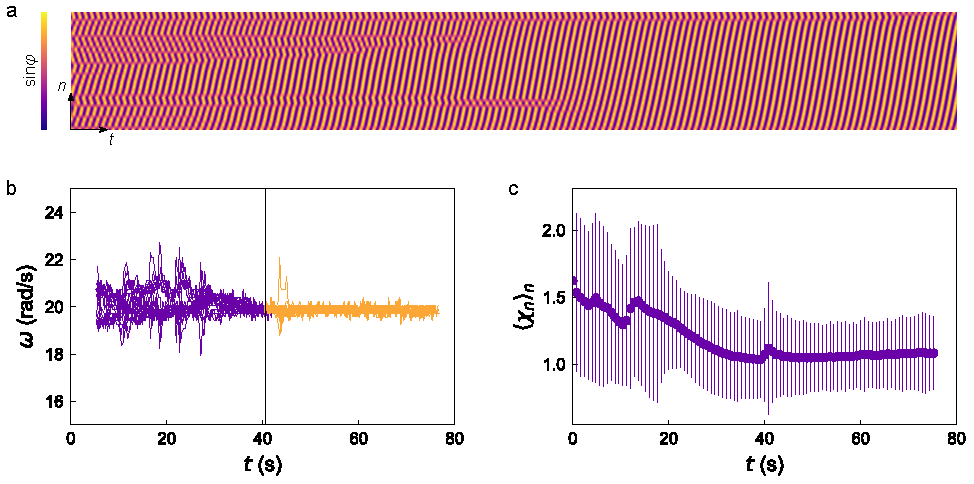
\includegraphics{figures/A2_SI1-v3.pdf}
    \caption{\textbf{Evolution of traveling waves.} (a) Full length space-time plot showing the development of traveling wave synchronization (see Figure 1d and Supplementary Movie 1). (b) Instantaneous oscillation frequency of each oscillator as a function of time during the development of synchronization. The onset of the fully synchronized state is denoted by the change in color from purple to yellow. (c) Average phase difference as a function of time during the development of synchronization. Error bars represent standard deviations in the phase difference. Data were collected for $N=23$, $a=1$ mm, $W=3$ mm, $L=25$ mm, and $V=19$ kV.}
    \label{fig:SI1}
\end{figure}


%%%%%%%%%%%%%%%%%%%%%%%%%%%%%%%%%%%%
\begin{figure}[p]
    \centering
    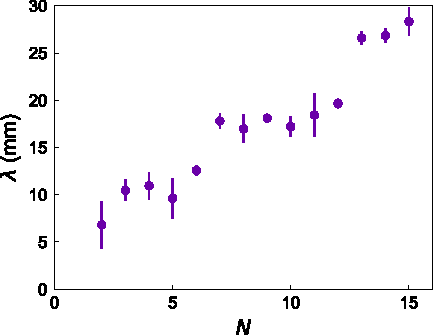
\includegraphics{figures/A2_SI2.pdf}
    \caption{\textbf{Dependence of wavelength on the number of oscillators.} Wavelength $\lambda$ (defined in the main text) as a function of the number of oscillators $N<N^*=15$. Error bars denote the standard deviation obtained over 50 cycles.  Data  were collected with $a=1$ mm, $L=25$ mm, $W=3$ mm, and $V=18$ kV.}
    \label{fig:SI2}
\end{figure}
%%%%%%%%%%%%%%%%%%%%%%%%%%%%%%%%%%%%

%%%%%%%%%%%%%%%%%%%%%%%%%%%%%%%%%%%%
\begin{figure}[p]
    \centering
    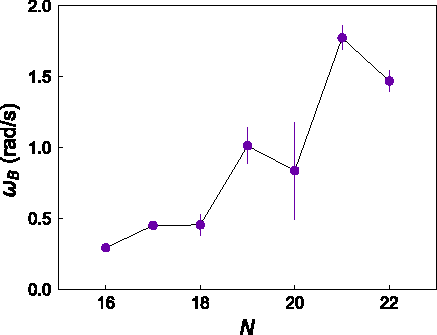
\includegraphics{figures/A2_SI3.pdf}
    \caption{\textbf{Dependence of breaking frequency on  oscillator number $N>N^*$.} Breaking frequency frequency $\omega_B$ as a function of the oscillator number $N>N^*=15$. Error bars denote standard deviations obtained over at least five breaking events. Data  were collected with $a=1$ mm, $L=25$ mm, $W=3$ mm, and $V=18$ kV.}
    \label{fig:SI3}
\end{figure}
%%%%%%%%%%%%%%%%%%%%%%%%%%%%%%%%%%%%


%%%%%%%%%%%%%%%%%%%%%%%%%%%%%%%%%%%%
\begin{figure}[p] 
    \centering
    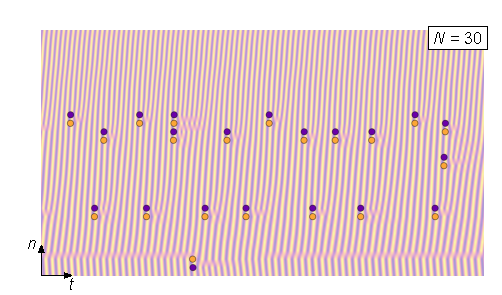
\includegraphics{figures/A2_SI4.pdf}
    \caption{\textbf{Space-time plot for $N\gg N^*$.} Space-time plot for  $N\gg N^*$ showing wave breaking at different locations and irregular time intervals. Wave breaks are characterized by edge dislocations highlighted by the markers, which show points in the space-time lattice with five-fold (purple) and seven-fold (yellow) coordination. Data were collected with $a=1$ mm, $L=25$ mm, $W=3$ mm, and $V=18$ kV. See also Supplementary Movie 5.}
    \label{fig:SI4}
\end{figure}
%%%%%%%%%%%%%%%%%%%%%%%%%%%%%%%%%%%%

%%%%%%%%%%%%%%%%%%%%%%%%%%%%%%%%%%%%
\begin{figure}[p]
    \centering
    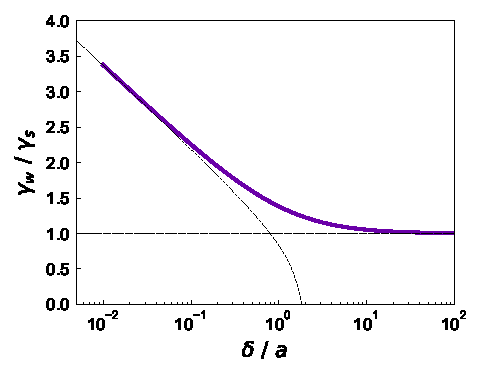
\includegraphics{figures/A2_drafCoefficient.pdf}
    \caption{\textbf{Friction coefficient for a sphere above a plane wall.} Friction coefficient $\gamma_w$ for a torque-free sphere of radius $a$ moving through a viscous fluid parallel a plane wall as a function of the surface separation $\delta$.  The friction coefficient is scaled by the Stokes drag, $\gamma_s=6\pi \eta a$, for a sphere in an unbounded fluid.  The solid curve shows the exact solution\autocite{ONeill1964a,Dean1963}; the dashed curves show the limiting behaviors for small and large surface separations.  At small separations ($\delta\ll a)$, the friction coefficient is well approximated by asymptotic expressions due to Goldman, Cox, and Brenner\autocite{Goldman1967a}.  A surface separation of $\delta = (6.4\times10^{-3})a=6.4~\mu$m would enhance the drag by the experimentally observed factor of 3.6.}
    \label{fig:SI6}
\end{figure}
%%%%%%%%%%%%%%%%%%%%%%%%%%%%%%%%%%%%


%%%%%%%%%%%%%%%%%%%%%%%%%%%%%%%%%%%%
\begin{figure}[p]
    \centering
    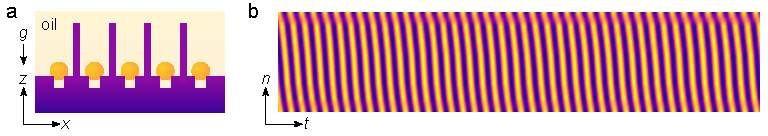
\includegraphics{figures/A2_SI5-v2.pdf}
    \caption{\textbf{Control experiments on the role of hydrodynamic interactions.} (a) Experiments were performed in which particles were separated by solid walls to eliminate hydrodynamic interactions between neighboring particles. (b) Space-time plot showing traveling wave synchronization in the absence of hydrodynamic interactions. Data were collected with  $N=8$, $a=1$ mm, $W=4$ mm, $L=25$ mm, and $V=19$ kV.}
    \label{fig:SI6}
\end{figure}
%%%%%%%%%%%%%%%%%%%%%%%%%%%%%%%%%%%%

%%%%%%%%%%%%%%%%%%%%%%%%%%%%%%%%%%%%
%%%%%%%%%%%%%%%%%%%%%%%%%%%%%%%%%%%%
\subsection{Supplementary Note 1: Amplitude dynamics}

In the main text, we model the particles as weakly-coupled phase oscillators and neglect the amplitude dynamics.  Here, we validate that approximation using numerical solutions of the corresponding ``exact'' model that includes amplitude dynamics.  In particular, we consider the dynamics of $N$ oscillators moving between two nearly parallel electrodes subject to a constant voltage $V$.  The electrode separation $L_i$ at the location of oscillator $i$ is assumed to vary linearly as $L_i=L_o - \Delta L[i + \tfrac{1}{2}(N+1)]$, where $L_o$ is the average separation and $\Delta L$ is the difference in the separation between neighboring oscillators.  The latter is related to the small angle $\theta$ between the electrodes as  $\Delta L / W =  \tan\theta \ll1$.  The external electric field acting on oscillator $i$ is approximated as $E_i=V/L_i$.

The position $h_i$ of oscillator $i$ is governed by the overdamped dynamics,
\begin{equation}
    \gamma \frac{d h_i}{d t} = q_i (E_i + E'_i),
\end{equation}
where $E'_i$ denotes the disturbance field due to neighboring particles.  The charge on oscillator $i$ changes instantaneously upon contact with the electrodes at $h_i=0$ and $h_i=L_i$. The resulting charge is
\begin{equation}
    q_i = \pm \frac{2}{3}\pi^3 \varepsilon a^2 (E_i + E'_i),
\end{equation}
where the positive sign applies at $h_i=0$ and the negative sign at $h_i=L_i$.  Again, the electric field acting on particle $i$ contains contributions from the applied field $E_i$ and from the disturbance field $E'_i$ due to neighboring particles.  In particular, the disturbance field acting on oscillator $i$ due to neighboring particles $j$ is approximated as
\begin{equation}
    E'_i = \sum_j -\frac{q_j}{L^2 \varepsilon} \sum_{m=1}^{\infty} m \sin\left(\frac{m\pi h_j}{L_j}\right) \cos\left(\frac{m\pi h_i }{L_i}\right) K_0\left(\frac{m \pi W}{L_o}\right),
\end{equation}
where the first sum is over nearest neighbors ($j=i-1$ and $i+1$) separated by a distance $W$.

It is convenient to non-dimensionalize this model by scaling lengths by $L_o$, fields by $E_o=V/L_o$, charges by $q_o=\tfrac{2}{3}\pi^3 \varepsilon a^2 E_o$, and time by $\gamma L_o/q_o E_o$.  The resulting dynamics are governed by four dimensionless parameters: (1) the number of oscillators $N$, (2) the oscillator spacing $W/L_o$, (3) electrode angle $\theta$, and (4) the coupling strength $a/W$.  We focus our analysis on the experimental conditions of Figure 2b, in which $N=15$, $W/L_o=0.12$, $\theta=1^{\circ}$, and $a/W=0.33$. The particle dynamics are integrated numerically using Mathematica's event handling feature to update the particle charges at each contact with an electrode.  At long times, the oscillators approach a steady periodic solution as illustrated in Figure \ref{fig:amplitude}.  Averaging the phase difference over one oscillation period, the results of this ``exact'' model are very well approximated by the simpler model based on weakly-coupled phase oscillators.  We note that the amplitude dynamics become more significant as the number of particles is increased from $N=10$ to $N=15$ towards the critical number of $N^*=16$.

\begin{figure}
    \centering
    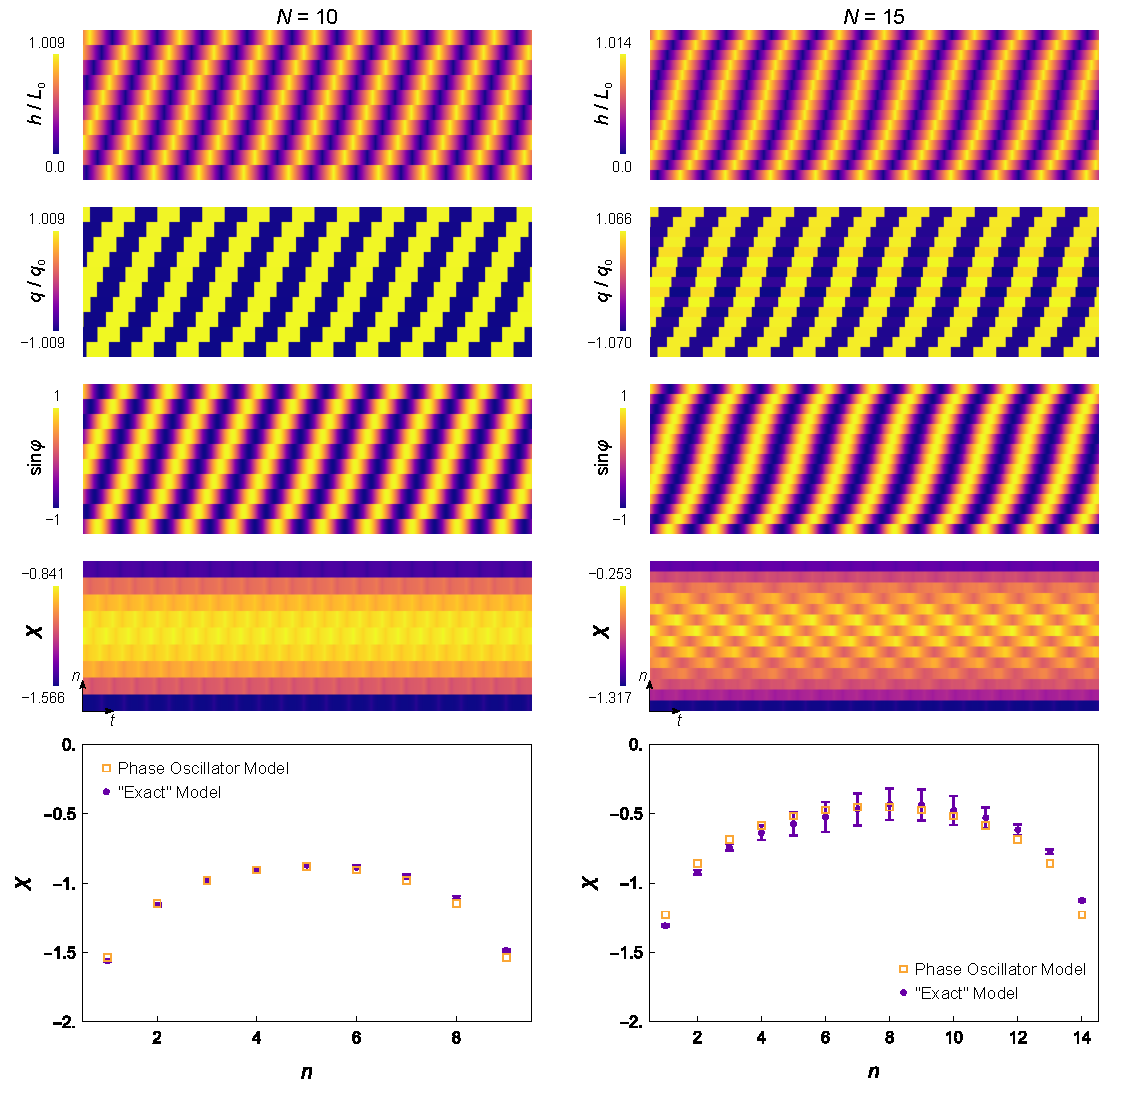
\includegraphics[width=\textwidth]{figures/A2_amplitudeDynamics.pdf}
    \caption{Numerical solution of the ``exact'' model for $N=10$ (left) and $N=15$ (right) oscillators.  The parameters are the same as those in Figure 3 of the main text: $W/L=0.12$, $a/W=0.33$, and $\theta=1^{\circ}$.  From top to bottom, the space-time plots show the particle position $h$ (scaled by the average electrode separation $L_o$), the particle charge $q$ (scaled by the Maxwell charge $q_o$), the sine of the phase $\sin\varphi$, and the phase difference $\chi$.  The plot shows the time-averaged phase difference $\chi$ as a function of the oscillator number $n$.}
    \label{fig:amplitude}
\end{figure}

\clearpage
\subsection{Supplementary Note 2: Stationary solution}

The stationary solution $f(\chi_n)=\tfrac{1}{2}\Delta n(n-N)$ is obtained by solving the following set of linear recurrence equations derived in the Methods,
\begin{align}
    \Delta &= -2 f_1 + f_2 , \label{eq:bc1}
    \\
    \Delta &= f_{n-1} - 2 f_n + f_{n+1} \quad \text{for } n=2,\dots,N-2, \label{eq:mid}
    \\
    \Delta &= f_{N-2} - 2 f_{N-1}, \label{eq:bc2}
\end{align}
where $f_n=f(\chi_n)$.  Equation (\ref{eq:mid}) has the following general solution
\begin{equation}
    f_n = C_1 + C_2 n + \frac{1}{2}\Delta n(n-1).
\end{equation}
The constants $C_1$ and $C_2$ are determined by substituting this result into the boundary conditions (\ref{eq:bc1}) and (\ref{eq:bc2}).  As the equations are linear, the resulting solution for $f_n$ is unique. However, when $|f_n| > f_{\max}$, there exists no value of the phase difference $\chi_n$ that satisfies the equation $f(\chi_n)=f_n$.  Alternatively, when $|f_n|<f_{\max}$, there exists two possible solutions for the phase difference---one with $f'(\chi_n)>0$ and another with $f'(\chi_n)<0$ as can be seen graphically in Figure 3b of the main text.

%%%%%%%%%%%%%%%%%%%%%%%%%%%%%%%%%%%%
\subsection{Supplementary Note 3: Stability of the stationary solution}

As noted above, there are two possible solutions for each of the $N-1$ phase differences.  In both experiment and simulations, we observed only one of these possible solutions in which $f'(\chi_n)<0$ for all $n$.  Here, we confirm the stability of this solution to small perturbations using a continuum approximation, in which the phase difference $\chi_n(t)$ is replaced by a continuous function $\chi(n,t)$. In this limit, the dynamics of the phase difference can be approximated as
\begin{equation}
    \frac{\partial \chi(n,t)}{\partial t} = -\frac{\partial^2 f(\chi(n,t))}{\partial n^2}  + \Delta, \label{eq:cont}
\end{equation}
subject to boundary conditions 
\begin{equation}
    f(\chi(0,t)) = f(\chi(N,t)) = 0.
\end{equation}
Note that the discrete equations for $\chi_n(t)$ correspond to a second order finite difference approximation of these continuous equations. The characteristic error introduced by this approximation is of order $(1/N)^2$, which becomes negligible for large $N$. The stationary solution $\chi_{\s}(n,t)$ is identical to that derived above for the discrete case
\begin{equation}
    \chi_{\s}(n) = \frac{1}{2} \Delta n(n-N).
\end{equation}
For small perturbations about this solution, we can approximate the function $f(\chi(n,t))$ by a first order Taylor expansion
\begin{equation}
    f(\chi(n,t)) = f(\chi_{\s}(n)) + f'(\chi_{\s}(n))[\chi(n,t)-\chi_{\s}(n)] + \dots
\end{equation}
Substituting this approximation into equation  (\ref{eq:cont}), we obtain the following diffusion equation
\begin{equation}
    \frac{\partial g}{\partial t} = -f'(\chi_{\s}(n)) \frac{\partial^2 g}{\partial n^2}, \label{eq:perturb}
\end{equation}
for the perturbation function $g(n,t)= f'(\chi_{\s}(n))[\chi(n,t)-\chi_{\s}(n)]$. Perturbations $g(n,t)$ evolve in time with a spatially dependent diffusivity $-f'(\chi_{\s}(n))$, which must be positive to ensure the decay of the perturbations and the stability of the stationary state.  Furthermore, if we approximate this diffusivity as constant, $-f'(\chi_{\s}(n))\sim f_{\max} / \chi_{\max}$, the characteristic relaxation time for equation (\ref{eq:perturb}) can be computed as $\tau \sim \chi_{\max} N^2 / \pi^2 f_{\max}$ as stated in the Methods.




\end{appendices}
\begin{appendices}

%Some Table of Contents entry formatting
\addtocontents{toc}{\protect\renewcommand{\protect\cftchappresnum}{\appendixname\space}}
\addtocontents{toc}{\protect\renewcommand{\protect\cftchapnumwidth}{6em}}

%Begin individual appendices, separated as chapters

\chapter{Supporting information for chapter 4}
In this appendix, firstly, we use perturbation theory to derive that fixed radius is requirement for microswimmers' effective navigation. Then the theoretical details are shown to solve the diffusion, hydrodynamics and motions of shape-shifting autophoretic clusters. We also investigate how the thermal noise influences the efficiency of navigation. Finally, we show how to define different target function to achieve navigation behaviors towards different directions 

\section{Equations of Motion}

As described in the main text, we consider a particle at location $\ve{x}_p=[x_p,y_p]$ with orientation $\theta$ moving with a linear velocity $\ve{U}$ and angular velocity $\Omega$.  The components of the linear velocity in the particle frame are parameterized as $\ve{U}=[U \cos\alpha, U\sin \alpha]$, where $U$ is the linear speed and the angle $\alpha$ describes the direction of motion in the particle frame.  The resulting particle dynamics are given by
\begin{align}
    \dot{\theta} &= \Omega \label{eq:theta}
    \\ 
    \dot{x}_p &= U \cos(\theta + \alpha) \label{eq:xp} 
    \\ 
    \dot{y}_p &= U \sin(\theta + \alpha)\label{eq:yp}
\end{align}	
The velocity parameters $U$, $\alpha$, and $\Omega$ are assumed to depend on the value of a scalar stimulus field $S(\ve{x},t)$ evaluated at the particle center---for example, $\alpha=\alpha(S(\ve{x}_p,t))$. Here, we consider the specific case of a uniform stimulus gradient in the $x$-direction such that $S(\ve{x})= G x$, where $G$ is the gradient magnitude. Dividing equations (\ref{eq:xp}) and (\ref{eq:yp}) by equation (\ref{eq:theta}), we can write the dynamics for the particle position in terms of its orientation $\theta$ 
\begin{align}
    \frac{d x_p}{d\theta} &= R \cos(\theta + \alpha) \label{eq:xp2} 
    \\ 
    \frac{d y_p}{d\theta} &= R \sin(\theta + \alpha)\label{eq:yp2}
\end{align}	
where $R=\Omega/U$ is the radius of curvature of the particle trajectory (in the particle frame). 

%%%%%%%%%%%%%%%%%%%%%%%%%%%%%%%%%%%%%%%%%
%%%%%%%%%%%%%%%%%%%%%%%%%%%%%%%%%%%%%%%%%
\subsection{Approximate Solution for Weak Gradients}

In the absence of a stimulus gradient ($G=0$), equations(\ref{eq:xp2}) and (\ref{eq:yp2}) describe a simple circular orbit of radius $R$
\begin{align}
    x_p(\theta) = C_1 + R \sin(\theta + \alpha) \label{eq:xp3} 
    \\
    y_p(\theta) = C_2 - R \cos(\theta + \alpha)\label{eq:yp3} 
\end{align}
where $C_1$ and $C_2$ are constants that describe the position of the particle at some initial orientation.  In a weak gradient ($G\neq 0$), the radius $R$ and phase $\alpha$ of the particle's circular motion are expected to evolve slowly in time.  To obtain the slow dynamics, we use a two-timing perturbation technique\autocite{Strogatz2015} that distinguishes a fast variable $\tau=\theta$ and a slow variable $T=\varepsilon \theta$ where $\varepsilon$ is a small parameter proportional to the gradient magnitude $G$. The particle position is then expanded as
\begin{equation}
    \ve{x}_p(\theta,\varepsilon) = \ve{x}_0(\tau,T) + \varepsilon \ve{x}_1(\tau,T) + O(\varepsilon^2)
\end{equation}
We substitute this expansion into equations (\ref{eq:xp2}) and (\ref{eq:yp2}) and collect like powers of $\varepsilon$. At zeroth order in $\varepsilon$, the solution is equivalent to equations (\ref{eq:xp3}) and (\ref{eq:yp3}) above. At first order in $\varepsilon$, the governing equations become
\begin{align}
    \partial_T x_0 + \partial_{\tau} x_1 = G x_0 \left[ R' \cos(\tau + \alpha) - R \alpha' \sin(\tau + \alpha)\right] \label{eq:xp4} 
    \\
    \partial_T y_0 + \partial_{\tau} y_1 = G x_0 \left[ R' \sin(\tau + \alpha) + R \alpha' \cos(\tau + \alpha)\right] \label{eq:yp4}
\end{align}
Averaging over the fast variable $\tau$ from 0 to $2\pi$, we obtain the following expressions for the drift velocity in the stimulus gradient    
\begin{align}
    \langle \partial_{\tau} x_1 \rangle &=  - \tfrac{1}{2} G R^2\alpha' \label{eq:drift}
    \\
    \langle \partial_{\tau} y_1 \rangle &= \tfrac{1}{2} G R R' \label{eq:drift2}
\end{align}
where the prime denotes differentiation with respective to the slow variable. To avoid net motion of the particle in the $y$ direction, the radius of the trajectory $R$ must be independent of the stimulus such that $R'=0$.  Equation (\ref{eq:drift}) provides an estimate of the drift velocity in the $x$-direction due to the changing orientation of the particle velocity in the stimulus landscape.  The accuracy of this approximation requires that drift velocity be slow relative to the circular motion of the particle, which implies that $G R\alpha' \ll 1$.  Figure \ref{fig:SimpleModel} highlights the performance of this analytical approximation for a specific response function $\alpha(S)$.
\begin{figure}[h]
    \centering
    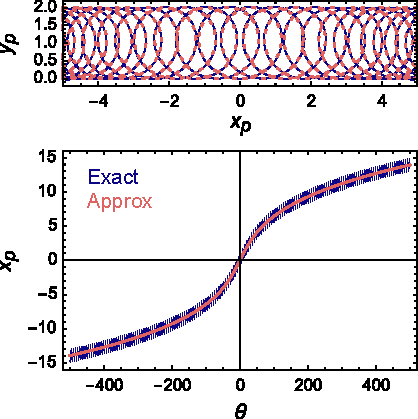
\includegraphics[width=9cm]{figures/A3_SimpleModel.pdf}
    \caption{Computed particle trajectory for $\alpha(S) = \arctan(-0.2 S)$ and $R=\text{constant}$ in a uniform stimulus gradient $S=G x$. Here, lengths are scaled by the curvature radius $R$ and stimuli by $GR$ (corresponding to $R\rightarrow1$ and $G\rightarrow1$). The solid purple curve shows the exact result; the dashed pink curve shows the slow dynamics described by equation (\ref{eq:drift}). The small parameter governing the accuracy of the approximation is $G R\alpha' = 0.2 \ll 1$.}
    \label{fig:SimpleModel}
\end{figure}


%%%%%%%%%%%%%%%%%%%%%%%%%%%%%%%%%%%%%%%%%
%%%%%%%%%%%%%%%%%%%%%%%%%%%%%%%%%%%%%%%%%
\subsection{Choice of Sensor Location}

The particle's velocity is assumed to depend on the stimulus magnitude evaluated at the particle center $\ve{x}_p$.  If the stimulus magnitude is instead evaluated at a different position on the particle $\ve{x}_s\neq \ve{x}_p$, the resulting dynamics will be slightly different.  However, such differences are negligible when the characteristic size of the particle is much smaller than the radius of its periodic orbit.  To show this, we consider how the drift velocity depends on the sensor position $\ve{x}_s$, at which the stimulus is ``sensed'' by the particle.  We assume that the particle has fixed response functions $R(S)$ and $\alpha(S)$ where $S = S(\ve{x}_s(t))$. In the particle frame, we defined the constant displacement between the sensor and the particle center as $\ve{x}_s-\ve{x}_p =[\delta \cos\beta, \delta \sin\beta]$.  The dynamics of equations (\ref{eq:xp2}) and (\ref{eq:yp2}) are modified as
\begin{align}
    \frac{d x_p}{d\theta} &= R(G x_s ) \cos(\theta + \alpha(G x_s))   
    \\ 
    \frac{d y_p}{d\theta} &= R(G x_s) \sin(\theta + \alpha(G x_s))
\end{align}	
where $x_s = x_p + \delta  \cos( \theta +\beta)$.  Following the same two-timing scheme described above, the first order equations (\ref{eq:xp4}) and (\ref{eq:yp4}) become
\begin{align}
    \partial_T x_0 + \partial_{\tau} x_1 = G \left[ x_0 + \delta \cos(\tau +\beta)\right] \left[ R' \cos(\tau + \alpha) - R \alpha' \sin(\tau + \alpha)\right]
    \\
    \partial_T y_0 + \partial_{\tau} y_1 = G \left[ x_0 + \delta \cos(\tau +\beta)\right] \left[ R' \sin(\tau + \alpha) + R \alpha' \cos(\tau + \alpha)\right]
\end{align}
Averaging over the fast variable $\tau$ from 0 to $2\pi$, we obtain the following expressions for the drift velocity in the stimulus gradient    
\begin{align}
    \langle \partial_{\tau} x_1 \rangle &= -\tfrac{1}{2} G R^2\alpha' \left( 1 + \frac{\delta}{R}\sin(\alpha-\beta) \right) + \tfrac{1}{2} G R R' \left( \frac{\delta}{R} \cos(\alpha-\beta) \right) \label{eq:xdrift2}
    \\
    \langle \partial_{\tau} y_1 \rangle &= \tfrac{1}{2} G R^2\alpha' \left( \frac{\delta}{R} \cos(\alpha-\beta) \right) + \tfrac{1}{2} G R R'\left( 1 + \frac{\delta}{R}\sin(\alpha-\beta) \right) \label{eq:ydrift2}
\end{align}
Changes in the location of the sensor give rise to corrections in the drift velocity of order $\delta/R$ relative to equations (\ref{eq:drift}) and (\ref{eq:drift2}).  Figure \ref{fig:SensorLocation} shows two computed particle trajectories with $\delta=0$ and $\delta = 0.1 R$ to illustrate the effect of sensor location on particle chemotaxis.
\section{Model Details for Rigid Self-phoretic Clusters}

We consider the self-phoretic propulsion of a rigid cluster of $N$ solid spheres of radii $a_j$. Each sphere $j$ releases a constant flux $A_j$ of a solute from its surface $\mathcal{S}_j$  
\begin{equation}
    -D \ve{n}\cdot \nabla c(\ve{x}) = A_j \quad \text{for} \quad \ve{x} \in \mathcal{S}_j \label{eq:bc1}
\end{equation}
where $D$ is the diffusivity, and $\ve{n}$ is the unit normal vector directed out from the surface.  The solute concentration $c(\ve{x})$ around the spheres quickly approaches a steady-state distribution governed by the Laplace equation
\begin{equation}
    \nabla^2 c = 0
\end{equation}
Far from the particle cluster, the solute concentration approaches a constant value $c^{\infty}$, which can be set to zero without loss of generality. 

The solute gradients generated by the particles produce a phoretic slip velocity tangent to the surface of each sphere 
\begin{equation}
    \ve{u}_s(\ve{x}) = \mu_j (\ve{I}-\ve{n}\ve{n}) \cdot \nabla c(\ve{x}) 
\end{equation}
where $\mu_j$ is the phoretic mobility of sphere $j$, and $\ve{I}$ is the identity tensor. At small Reynolds numbers, the fluid velocity $\ve{u}(\ve{x})$ surrounding the particle is governed by the Stokes equations
\begin{equation}
    0 = -\nabla p + \eta \nabla^2 \ve{u} \quad \text{and}\quad \nabla\cdot\ve{u} = 0
\end{equation}
where $\eta$ is the fluid viscosity.  The cluster of spheres moves as a rigid body with linear velocity $\ve{U}$ and angular velocity $\ve{\Omega}$.  At the surface of each sphere $j$, the fluid velocity is equal to that of the sphere plus the slip velocity  
\begin{equation}
    \ve{u}(\ve{x}) = \ve{U} + \ve{\Omega}\times(\ve{x}_j - \ve{x}_p) + \ve{u}_s(\ve{x}) \quad \text{for} \quad \ve{x} \in \mathcal{S}_j
\end{equation}
where $\ve{x}_p$ denotes the center of the composite particle.  Far from the particle, the fluid is stationary.  Finally, the velocities $\ve{U}$ and $\ve{\Omega}$ are determined by the condition that the net force and torque on the particle vanish
\begin{equation}
    0 = \int_{\mathcal{S}} (\ve{\sigma}\cdot\ve{n}) \mathrm{d}\mathcal{S}  \quad \text{and} \quad 0 = \int_{\mathcal{S}} (\ve{x}-\ve{x}_p)\times (\ve{\sigma}\cdot\ve{n} )\mathrm{d}\mathcal{S}  \label{eq:noForceTorque}
\end{equation}
where $\ve{\sigma} = -\nabla p + \eta(\nabla\ve{u}+\nabla\ve{u}^T)$ is the stress tensor.

%%%%%%%
%%%%%%%%   
%%%%%%%%
%%%%%%%%%%
%%%%%%%%%%
%%%%%%%%%%%
%%%%%%%%%%
%%%%%%%%%%
%%%%%%%%%%
%%%%%%%
%%%%%%%%
%%%%%%%%
%%%%%%%%%%
%%%%%%%%%%
%%%%%%%%%%%
%%%%%%%%%%
%%%%%%%%%%
%%%%%%%%%%
%%%%%%%
%%%%%%%%
%%%%%%%%
%%%%%%%%%%
%%%%%%%%%%
%%%%%%%%%%%
%%%%%%%%%%
%%%%%%%%%%
%%%%%%%%%%
\subsection{Diffusion Problem}

To approximate the solution to the diffusion problem, we start from the following integral solution for the concentration field
\begin{equation}
    c(\ve{x}) - c^{\infty}(\ve{x}) = \int_{\mathcal{S}} \left\{ c(\ve{y})[\ve{n}(\ve{y})\cdot \nabla_y G(\ve{y},\ve{x})]  -  G(\ve{y},\ve{x}) [\ve{n}(\ve{y})\cdot \nabla c(\ve{y})] \right\} d \mathcal{S}(\ve{y})
\end{equation}
where $\ve{n}$ is the unit normal vector directed into the fluid, and $G(\ve{y},\ve{x})$ is the Green's function for the concentration at $\ve{y}$ due to a point source at $\ve{x}$.  Expanding the Green's function in a Taylor series in $\ve{y}$ about the center $\ve{x}_j$ of each sphere $j$, we obtain
\begin{equation}
    c(\ve{x}) - c^{\infty}(\ve{x})  = \sum^N_{j=1} \left[ C_0^j G(\ve{x}_j,\ve{x}) + \ve{C}_1^j\cdot \nabla_y G(\ve{y},\ve{x})\rvert_{\ve{y}=\ve{x}_j} + \dots \right] 
\end{equation}
where the first and second moments are 
\begin{gather}
    C_0^j = \int_{\mathcal{S}_j} - \ve{n}(\ve{y})\cdot \nabla c(\ve{y})d \mathcal{S}(\ve{y})
    \\
    \ve{C}_1^j = \int_{\mathcal{S}_j} \left\{ c(\ve{y})\ve{n}(\ve{y}) - (\ve{y}-\ve{x}_j)[\ve{n}(\ve{y})\cdot \nabla c(\ve{y})] \right\} d \mathcal{S}(\ve{y})
\end{gather}
We have truncated this multipole expansion at the dipole level; however, higher order contributions can be derived in a similar manner. Substituting the boundary condition (\ref{eq:bc1}) for the surface flux, the above moments can be simplified as
\begin{gather}
    C_0^j = \frac{4\pi a_j^2 A_j}{D}
    \\
    \ve{C}_1^j = \int_{\mathcal{S}_i} c(\ve{y})\ve{n}(\ve{y}) d \mathcal{S}(\ve{y})
\end{gather}
In an unbounded domain, the Green's function is $G(\ve{y},\ve{x}) = (4\pi \lvert \ve{y}-\ve{x}\rvert)^{-1}$, and the multipole expansion for the concentration becomes
\begin{equation}
    c(\ve{x}) - c^{\infty}(\ve{x})  = \frac{1}{4\pi} \sum^N_{j=1} \left[ \frac{C_0^j}{\lvert\ve{x}-\ve{x}_j\rvert}  + \frac{\ve{C}_1^j\cdot(\ve{x}-\ve{x}_j)}{\lvert\ve{x}-\ve{x}_j\rvert^3} + \dots \right] \label{eq:multipole}
\end{equation}

To solve for the dipole moments $\ve{C}_1$, we make used of the following relations (so-called Fax\'en laws\autocite{Bonnecaze1990,OBrien1979}) for a sphere $i$ in an external concentration field $c'(\ve{x})$ 
\begin{gather}
    c(\ve{x}_i) - c'(\ve{x}_i) = \frac{C_0^i}{4\pi a_i}  \label{eq:faxen1}
    \\
    -\nabla c'(\ve{x}_i) = \frac{\ve{C}_1^i}{2\pi a_i^3}  \label{eq:faxen2}
\end{gather}
Here, the external concentration and its gradient are evaluated at the center of the sphere in its absence; the particle concentration $c(\ve{x}_i)$ is defined as the average concentration on the surface of the sphere
\begin{equation}
    c(\ve{x}_i) \equiv \frac{1}{4\pi a_i^2} \int_{\mathcal{S}_i} c(\ve{x}) d\mathcal{S}(\ve{x}) 
\end{equation}
Combing the Fax\'en laws (\ref{eq:faxen1}) and (\ref{eq:faxen2}) with the multipole expansion (\ref{eq:multipole}), we obtain the following linear equations
\begin{equation}
    \begin{bmatrix} c_i-c^{\infty}_i \\ c_j-c^{\infty}_j \\ \vdots \\ -\nabla c^{\infty}_i \\ -\nabla c^{\infty}_j \\ \vdots \end{bmatrix} = 
    \begin{bmatrix} 
        a_{ii} & a_{ij} & \cdots &\ve{\tilde{b}}_{ii} & \ve{\tilde{b}}_{ij} & \cdots \\
        a_{ji} & a_{jj} & \cdots & \ve{\tilde{b}}_{ji} & \ve{\tilde{b}}_{jj} & \cdots \\
        \vdots & \vdots & & \vdots & \vdots &  \\
        \ve{b}_{ii} & \ve{b}_{ij} & \cdots & \ve{c}_{ii} & \ve{c}_{ij} & \cdots \\
        \ve{b}_{ji} & \ve{b}_{jj} & \cdots & \ve{c}_{ji} & \ve{c}_{jj} & \cdots \\
        \vdots & \vdots & & \vdots & \vdots &  \\
    \end{bmatrix}
    \cdot
    \begin{bmatrix} C^i_0 \\ C^j_0 \\ \vdots \\ \ve{C}^i_1 \\ \ve{C}^j_1 \\ \vdots \end{bmatrix} \label{eq:grandPotential}
\end{equation}
where $c_i=c(\ve{x}_i)$ and $\nabla c^{\infty}_i=\nabla c^{\infty}(\ve{x}_i)$.  The quantities $a$, $\ve{\tilde{b}}$, $\ve{b}$, and $\ve{c}$ are components of the grand potential tensor (so-called in electrostatics\autocite{Bonnecaze1990})
\begin{gather}
    a_{ii} = \frac{1}{4\pi a_i} \quad \text{and} \quad  a_{ij} = a_{ji} = \frac{1}{4\pi r_{ij}}
    \\
    \ve{\tilde{b}}_{ii} = \ve{b}_{ii} = 0 \quad \text{and} \quad \ve{\tilde{b}}_{ij} = -\ve{\tilde{b}}_{ji} = -\ve{b}_{ij} = \ve{b}_{ji} = \frac{\ve{\hat{r}}_{ij}}{4\pi r_{ij}^2} 
    \\
    \ve{c}_{ii} = \frac{\ve{I}}{2\pi a_i^3} \quad \text{and} \quad \ve{c}_{ij} = \ve{c}_{ji} =  \frac{1}{4\pi r_{ij}^3} \left(\ve{I} - 3\ve{\hat{r}}_{ij}\ve{\hat{r}}_{ij}\right)
\end{gather}
with $\ve{r}_{ij} = \ve{x}_i - \ve{x}_j$ and $\ve{\hat{r}}_{ij} = \ve{r}_{ij}/ r_{ij}$.  In the present context, the external concentration field is absent (i.e., $c^{\infty}(\ve{x})=0$) and the monopole moments $C_0$ are known.  We can therefore solve equation (\ref{eq:grandPotential}) for the unknown dipole moments $\ve{C}_1$.  This approach is equivalent to the method of reflections detailed by Michelin \emph{et al.}\autocite{varma2018clustering}  The magnitude of dipole moment  scales as $C_1^j \propto (a/d)^2$ where $a$ is a typical sphere radius and $d$ is a characteristic separation between spheres. Truncating the multipole expansion at the dipole level introduces errors of order $(a/d)^7$ in estimating the dipole moments $\ve{C}_1^j$.    

%%%%%%%%%%%%%%%%%%%%%%%%%%%%%%%%%%%%%%%%%
%%%%%%%%%%%%%%%%%%%%%%%%%%%%%%%%%%%%%%%%%
\subsection{Hydrodynamic Problem}

Owing to the linearity of the Stokes equations, the stress tensor $\ve{\sigma}$ can be decomposed as the sum of two parts: first that of the moving spheres with no slip at their surface (denoted $\ve{\sigma}'$), and second that of stationary spheres with a prescribed slip velocity at their surface (denoted $\ve{\sigma}''$).  The no force and torque conditions (\ref{eq:noForceTorque}) can then be written as
\begin{gather}
    0 = \sum_j \ve{F}'_j +  \int_{\mathcal{S}} (\ve{\sigma}''\cdot\ve{n}) \mathrm{d}\mathcal{S} \label{eq:noForce}
    \\
    0 = \sum_j \left[(\ve{x}_j-\ve{x}_p)\times \ve{F}'_j + \ve{L}'_j\right] +  \int_{\mathcal{S}} (\ve{x}-\ve{x}_p)\times(\ve{\sigma}''\cdot\ve{n}) \mathrm{d}\mathcal{S}   \label{eq:noTorque}
\end{gather}
where $\ve{F}'_j$ and $\ve{L}'_j$ are the hydrodynamic drag force and torque on sphere $j$ due to its motion and that of the neighboring spheres (in the absence of activity). The integrals can be simplified by use of the Lorentz reciprocal theorem,\autocite{Kim2005} which relates the two flows $\ve{u}'$ and $\ve{u}''$ as 
\begin{equation}
    \int_{\mathcal{S}} \ve{u}'\cdot(\ve{\sigma}''\cdot\ve{n})  \mathrm{d}\mathcal{S} =  \int_{\mathcal{S}} \ve{u}''\cdot(\ve{\sigma}'\cdot\ve{n}) \mathrm{d}\mathcal{S} \label{eq:lorentz}
\end{equation}
The velocity $\ve{u'}$ at a point $\ve{x}$ on the surface of the rigid particle is $\ve{u'}=\ve{U}+\ve{\Omega}\times(\ve{x}-\ve{x}_p)$. Additionally, the normal stress on the surface of sphere $j$ is  $\ve{\sigma}'\cdot \ve{n}_j= -\tfrac{3\eta}{2a_j}\ve{U}_j-3\eta\ve{\Omega} \times\ve{n}_j$, where  $\ve{U}_j = \ve{U} +\ve{\Omega}\times(\ve{x}_j-\ve{x}_p)$ is the velocity of sphere $j$, and $\ve{n}_j$ is the unit normal directed out from the sphere.\autocite{Stone1996} Substituting these quantities into equation (\ref{eq:lorentz}) and collecting like terms in $\ve{U}$, we obtain
\begin{equation}
    \int_{\mathcal{S}} (\ve{\sigma}''\cdot\ve{n}) \mathrm{d}\mathcal{S}  = -\sum_j 6\pi\eta a_j \ve{U}_j^A \quad \text{with}\quad \ve{U}_j^A \equiv \frac{1}{4\pi a_j^2}\int_{\mathcal{S}_j} \ve{u}_s\mathrm{d}\mathcal{S} \label{eq:intForce}
\end{equation}
where $\ve{U}^A_j$ is the ``active'' linear velocity of sphere $j$. Similarly, we can collect terms in $\ve{\Omega}$ to obtain
\begin{equation}
    \int_{\mathcal{S}}(\ve{x}-\ve{x}_p)\times(\ve{\sigma}''\cdot\ve{n}) \mathrm{d}\mathcal{S} = -\sum_j\left[  6 \pi \eta a_j (\ve{x}_j-\ve{x}_p)\times\ve{U}^A_j  + 8\pi\eta a_j^3\ve{\Omega}^{A}_j\right] \label{eq:intTorque}
\end{equation}
where the ``active'' angular velocity is 
\begin{equation}
    \ve{\Omega}^{A}_j = \frac{3}{8\pi a_j^4}\int_{\mathcal{S}_j} (\ve{x}-\ve{x}_j) \times \ve{u}_s\mathrm{d}\mathcal{S}
\end{equation}
Substituting equations (\ref{eq:intForce}) and (\ref{eq:intTorque}) into equations (\ref{eq:noForce}) and (\ref{eq:noTorque}), we obtain 
\begin{gather}
    \sum_j \ve{F}'_j  = \sum_j 6\pi \eta a_j \ve{U}^A_j \label{eq:motion1}
    \\
    \sum_j \left[(\ve{x}_j-\ve{x}_p)\times \ve{F}'_j + \ve{L}'_j\right]  = \sum_j  \left(6 \pi \eta a_j (\ve{x}_j-\ve{x}_p)\times\ve{U}^A_j  - 8\pi\eta a_j^3\ve{\Omega}^{A}_j\right) \label{eq:motion2}
\end{gather}

The forces $\ve{F}'_j$ and torques $\ve{L}'_j$ on the solid spheres due to their motion through the fluid (in the absence of activity) are related to the particle velocities $\ve{U}$ and $\ve{\Omega}$ by the hydrodynamic resistance tensor
\begin{equation}
    \begin{bmatrix} \ve{F}'_i \\ \ve{F}'_j \\ \vdots \\ \ve{L}'_i \\ \ve{L}'_j \\ \vdots \end{bmatrix} = 
    \begin{bmatrix} 
        \ve{A}_{ii} & \ve{A}_{ij} & \cdots & \ve{\tilde{B}}_{ii} & \ve{\tilde{B}}_{ij} & \cdots \\ 
        \ve{A}_{ji} & \ve{A}_{jj} & \cdots & \ve{\tilde{B}}_{ji} & \ve{\tilde{B}}_{jj} & \cdots \\  
        \vdots  & \vdots & & \vdots & &  & \\ 
        \ve{B}_{ii} & \ve{B}_{ij} & \cdots & \ve{C}_{ii} & \ve{C}_{ij} & \cdots \\ 
        \ve{B}_{ji} & \ve{B}_{jj} & \cdots & \ve{C}_{ji} & \ve{C}_{jj} & \cdots \\  
        \vdots  & & & \vdots & &  &  
    \end{bmatrix} 
    \cdot
    \begin{bmatrix} \ve{U}_i \\ \ve{U}_j \\ \vdots \\ \ve{\Omega}_i \\ \ve{\Omega}_j \\ \vdots \end{bmatrix}\label{eq:stokes}
\end{equation}
For rigid body motion, the linear and angular velocities of the spheres are related to that of the cluster as $\ve{U}_j=\ve{U}+\ve{\Omega}\times(\ve{x}_j - \ve{x}_p)$ and $\ve{\Omega}_j=\ve{\Omega}$.  Substituting these expressions into equation (\ref{eq:stokes}), we obtain the following relation between the total force and torque on the particle and its linear and angular velocity
\begin{equation}
    \begin{bmatrix} \ve{F}' \\ \ve{L}' \end{bmatrix} = 
    \begin{bmatrix} 
        \ve{A} & \ve{\tilde{B}} \\ 
        \ve{B} & \ve{C} 
    \end{bmatrix} 
    \cdot
    \begin{bmatrix} \ve{U} \\ \ve{\Omega} \end{bmatrix}\label{eq:stokesParticle}
\end{equation}
where the components of the particle resistance tensor are 
\begin{gather}
    \ve{A} = \sum_{i,j} \ve{A}_{ij} \label{eq:A}
    \\
    \ve{\tilde{B}} = \ve{B}^T = \sum_{i,j} \left[(\ve{x}_j -\ve{x}_p) \times \ve{A}_{ij} + \ve{\tilde{B}}_{ij} \right] \label{eq:B}
    \\
    \ve{C} = \sum_{i,j}\left\{(\ve{x}_j -\ve{x}_p) \times [(\ve{x}_j -\ve{x}_p) \times \ve{A}_{ij}] + \ve{C}_{ij}\right\} \label{eq:C}
\end{gather}
Here, the cross products between a vector and a second order tensor indicate $(\ve{a}\times\ve{B})_{mn}=\varepsilon_{mpq} a_p B_{qn}$ where $\varepsilon_{mpq}$ is the alternating unit tensor.  Using the particle resistance tensor, the equations of motion (\ref{eq:motion1}) and (\ref{eq:motion2}) become
\begin{gather}
    \ve{A}\cdot \ve{U} + \ve{\tilde{B}} \cdot \ve{\Omega} = \sum_j 6\pi \eta a_j \ve{U}^A_j
    \\
    \ve{B}\cdot \ve{U} + \ve{C} \cdot \ve{\Omega}  = \sum_j  \left(6 \pi \eta a_j (\ve{x}_j-\ve{x}_p)\times\ve{U}^A_j  - 8\pi\eta a_j^3\ve{\Omega}^{A}_j\right)
\end{gather}

These equations for the particle velocity are exact; we now proceed to make some simplifying approximations to obtain the leading order contributions to the propulsion velocity when the separation between spheres is large relative to their size (i.e., $a/d\ll 1$).

To approximate the resistance tensor, we construct a truncated approximation to the corresponding mobility tensor that includes only the leading order hydrodynamic interactions between the spheres
\begin{equation}
    \begin{bmatrix} \ve{U}_i \\ \ve{U}_j \\ \vdots \\ \ve{\Omega}_i \\ \ve{\Omega}_j \\ \vdots \end{bmatrix}\label{eq:mobility}
    =
    \begin{bmatrix} 
        \ve{a}_{ii} & \ve{a}_{ij} & \cdots & \ve{\tilde{b}}_{ii} & \ve{\tilde{b}}_{ij} & \cdots \\ 
        \ve{a}_{ji} & \ve{a}_{jj} & \cdots & \ve{\tilde{b}}_{ji} & \ve{\tilde{b}}_{jj} & \cdots \\  
        \vdots  & \vdots & & \vdots & &  & \\ 
        \ve{b}_{ii} & \ve{b}_{ij} & \cdots & \ve{c}_{ii} & \ve{c}_{ij} & \cdots \\ 
        \ve{b}_{ji} & \ve{b}_{jj} & \cdots & \ve{c}_{ji} & \ve{c}_{jj} & \cdots \\  
        \vdots  & & & \vdots & &  &  
    \end{bmatrix} 
    \cdot
    \begin{bmatrix} \ve{F}'_i \\ \ve{F}'_j \\ \vdots \\ \ve{L}'_i \\ \ve{L}'_j \\ \vdots \end{bmatrix} 
\end{equation}
Here, the components of the mobility tensor are approximated as 
\begin{gather}
    \ve{a}_{ii} = \frac{1}{6\pi \eta a_i} \quad \text{and} \quad \ve{a}_{ij} = \frac{1}{8\pi \eta r_{ij}} (\ve{I} +\frac{ \ve{\hat{r}}_{ij}\ve{\hat{r}}_{ij}}{r_{ij}^2}    ) + \mathcal{O}(r^{-3}_{ij})
    \\
    \ve{\tilde{b}}_{ii} =\ve{b}_{ii} = 0 \quad \text{and} \quad \ve{\tilde{b}}_{ij} = \ve{b}_{ij} = 0 + \mathcal{O}(r^{-2}_{ij})
    \\
    \ve{c}_{ii} = \frac{1}{8\pi \eta a^3_i} \quad \text{and} \quad \ve{c}_{ij} = 0 + \mathcal{O}(r^{-3}_{ij})
\end{gather}
This truncated approximation to the mobility tensor is evaluated and inverted to obtain the the approximate resistance tensor.  From the diffusion problem above, the active linear velocity can be evaluated as 
\begin{equation}
    \ve{U}_j^A = -\frac{\mu_j \ve{C}_1^j}{2 \pi a_j^3}
\end{equation}
The active angular velocity $\ve{\Omega}_j^A$ depends on the second order moment $\ve{C}_2^j$, which is of order $(a/d)^3$ and neglected in our present analysis.


%%%%%%%%%%%%%%%%%%%%%%%%%%%%%%%%%%%%%%%%%
%%%%%%%%%%%%%%%%%%%%%%%%%%%%%%%%%%%%%%%%%
%%%%%%%%%%%%%%%%%%%%%%%%%%%%%%%%%%%%%%%%%
\clearpage
\section{Definition of Standard Shapes for Shape-shifting Particles}

In a shape-shifting cluster, the relative positions and orientations of the spheres are characterized by a single degree of freedom parameterized by $s$. To describe the kinematics of this shape-changing particle, we introduce two coordinate systems: the lab frame $\ve{x}=[x,y,z]$ and the particle frame $\ve{x}'=[x',y',z']$.  If $\ve{v}$ is a vector in the lab frame, then $\ve{v}'=\ve{R}\ve{v}$ is the same vector in the particle frame, where $\ve{R}$ is a rotation matrix that characterizes the relative orientation of the two frames (e.g., specified by the unit quaternion $\ve{q}$).  The position of sphere $j$ in the lab frame is given by 
\begin{equation}
    \ve{x}_j = \ve{x}_p + \ve{R}^T\ve{x}'_j
\end{equation}
where $\ve{x}_p$ is the center of the particle in the lab frame.  The positions of the spheres in the particle frame $\ve{x}'_j$ depend on the shape parameter $s$; the functions $\ve{x}'_j(s)$ define the standard shapes of the composite particle.\autocite{Shapere1989} Upon changes in the shape parameter $s$, the position of sphere $j$ changes as 
\begin{gather}
    \frac{d\ve{x}_j}{d s} = \frac{d \ve{x}_p}{d s} + \frac{d\ve{R}^T}{d s}\ve{x}'_j + \ve{R}^T\frac{d \ve{x}'_j}{ds}
    \\
    \frac{d\ve{x}_j}{d s} = \frac{d \ve{x}_p}{d s} + \frac{d\ve{R}^T}{d s} \ve{R}(\ve{x}_j-\ve{x}_p) + \ve{R}^T\frac{d \ve{x}'_j}{ds}
\end{gather}
The first and second terms describe rigid body translation and rotation through the fluid; the third describes additional motions due to shape change. Importantly, the standard shapes $\ve{x}'_j(s)$ can be defined such that the particle frame does not translate or rotate due to shape change---that is,
\begin{equation}
    \frac{d \ve{x}_p}{d s} = 0 \quad \text{and} \quad \frac{d\ve{R}^T}{d s} = 0
\end{equation}
for all $s$.  Moreover, since $\ve{x}_p$ and $\ve{R}$ are independent of the shape parameter, we are free to choose $\ve{x}_p=0$ and $\ve{R}=\ve{I}$ without loss of generality.  The use of this coordinate system ensures that particle motion is due entirely to phoretic propulsion.

To identify the standard shapes $\ve{x}'_j(s)$,  we start with a third reference frame, in which the positions of the spheres given by known functions $\ve{x}''_j(s)$.  The position and velocity of the sphere $j$ in the lab frame is expressed as 
\begin{gather}
    \ve{x}_j = \ve{x}'_p + \ve{R}'^T \ve{x}''_j 
    \\
    \frac{d\ve{x}_j}{ds} = \frac{d \ve{x}'_p}{ds} + \frac{d\ve{R}'^T}{d s} \ve{R}'(\ve{x}_j-\ve{x}'_p) + \ve{R}'^T\frac{d \ve{x}''_j}{ds} \label{eq:velocity}
\end{gather}
We substitute equation (\ref{eq:velocity}) for the sphere velocity into equation (\ref{eq:stokes}) for the corresponding forces and torques.  Changes in the configuration of the spheres are driven internally such that there is zero net force and torque on the composite particle.  Moreover, we assume that the relative orientations of the spheres do not change during shape-shifting (i.e., $\ve{\Omega}_i=\ve{\Omega}_j$ for all spheres pair $i$ and $j$). With these assumptions, the linear and angular velocity of the particle reference frame ($\ve{x}_p'$ and $\ve{R}'$) are governed by
\begin{gather}
    \ve{A}\ve{U} + \ve{\tilde{B}} \ve{\Omega} = -\sum_{i,j} \ve{A}_{ij} \ve{R}'^T \frac{d \ve{x}_j''}{d s} \label{eq:noForceShape}
    \\
    \ve{B}\ve{U} + \ve{C} \ve{\Omega} = -\sum_{i,j}\left[(\ve{x}_i-\ve{x}_p') \times \ve{A}_{ij} + \ve{B}_{ij}\right] \ve{R}'^T \frac{d \ve{x}_j''}{d s} \label{eq:noTorqueShape}
\end{gather}
where the components of the resistance tensor are given by equations (\ref{eq:A}), (\ref{eq:B}), and (\ref{eq:C}).
Starting from some initial condition $\ve{x}'_p(s_0)=0$ and $\ve{R}'(s_0) = \ve{I}$ for a shape parameter $s=s_0$, the dynamics of equations (\ref{eq:noTorqueShape}) and (\ref{eq:noForceShape}) can be evaluated numerically to determine $\ve{x}'_p(s)$ and $\ve{R}'(s)$.  The desired standard shapes $\ve{x}_j(s)$ are then given by
\begin{equation}
    \ve{x}_j(s) = \ve{x}_p' + \ve{R}'^T\ve{x}_j''
\end{equation}
For each shape $\ve{x}_j(s)$, the autophoretic velocity can be computed as detailed in the previous section by treating the particle as a rigid cluster.  In this way, we identify the response functions needed to describe particle motion on the stimulus landscape.

%%%%%%%%%%%%%%%%%%%%%%%%%%%%%%%%%%%%%%%%%
%%%%%%%%%%%%%%%%%%%%%%%%%%%%%%%%%%%%%%%%%
%%%%%%%%%%%%%%%%%%%%%%%%%%%%%%%%%%%%%%%%%
\clearpage
\section{Designed Cluster Moving Down the Gradient}

The objective function of equation (3) in the main text ensures that the particle will move parallel to the gradient direction; however, it does not specify the direction of motion up or down the gradient.  For the three sphere cluster considered in Figure 3, the optimal geometry combined with the specific sigmoidal relation between the shape parameter $s$ and the stimulus $S$ leads to autonomous navigation up the gradient (i.e., positive chemotaxis). To design the opposite behavior, we introduce an additional constraint to the optimization problem that the orientation of the propulsion velocity $\alpha$ must increase with the shape parameter $s$---that is, $d\alpha/ds>0$.  With this constraint, optimization of the design variables $\ve{d}$ to minimize variations in the specified radius $R_0$ leads to a new particle geometry that exhibits a negative chemotactic response (Fig.\ \ref{fig:negChemo}). 

\vspace{2cm}

\begin{figure}[h]
    \centering
    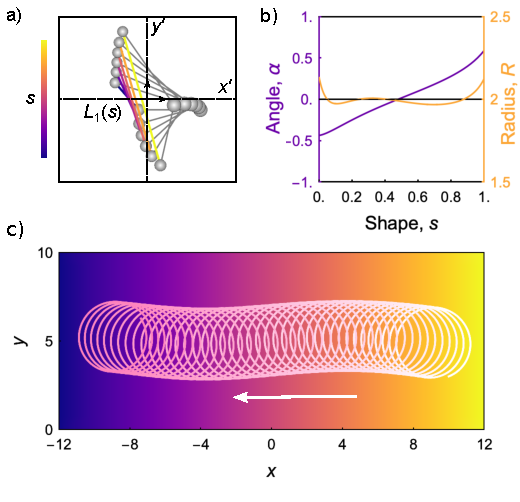
\includegraphics[width=9cm]{figures/A3_FigureS3.pdf}
    \caption{Design of a three-sphere cluster with a negative chemotactic response. (a) Standard shapes for the optimal design for different values of the shape parameter $s=(L_1-L_{\min})/(L_{\max}-L_{\min})\in [0,1]$. During optimization, we prescribe the lengths $L_3=0.6$, $L_{\min}=0.35$, $L_{\max}=1.35$ and $R_0=2$; the optimal design identified is $a_1=0.0562$, $a_2=0.0516$, $a_3=0.0683$, and $L_2=0.874$. (b) Computed response functions $\alpha(s)$ and $R(s)=U(s)/\Omega(s)$ for the standard shapes in (a). (c) Computed particle trajectory on a uniform stimulus gradient $S(\ve{x})=Gx$ of magnitude $G=0.2$; the shape parameter is assume to vary with the local stimulus as $s = (1+ e^{-S})^{-1}$.}
    \label{fig:negChemo}
\end{figure}

%%%%%%%%%%%%%%%%%%%%%%%%%%%%%%%%%%%%%%%%%
%%%%%%%%%%%%%%%%%%%%%%%%%%%%%%%%%%%%%%%%%
%%%%%%%%%%%%%%%%%%%%%%%%%%%%%%%%%%%%%%%%%
\clearpage
\section{Designed Cluster Moving Perpendicular to the Gradient}

To design clusters that move perpendicular to the gradient direction, we use a different objective function that characterizes the variations in the propulsion angle $\alpha$ about its mean value (which can be set to zero without loss of generality)
\begin{equation}
    O(\ve{d}) = \langle \alpha(s,\ve{d})^2 \rangle_s - \langle \alpha(s,\ve{d}) \rangle^2_s
\end{equation}
Moreover, we constrain the quantity $d R/d s$ to be positive or negative to control the direction of motion perpendicular to the gradient (Fig. \ref{fig:perpChemo}).

\begin{figure}[h]
    \centering
    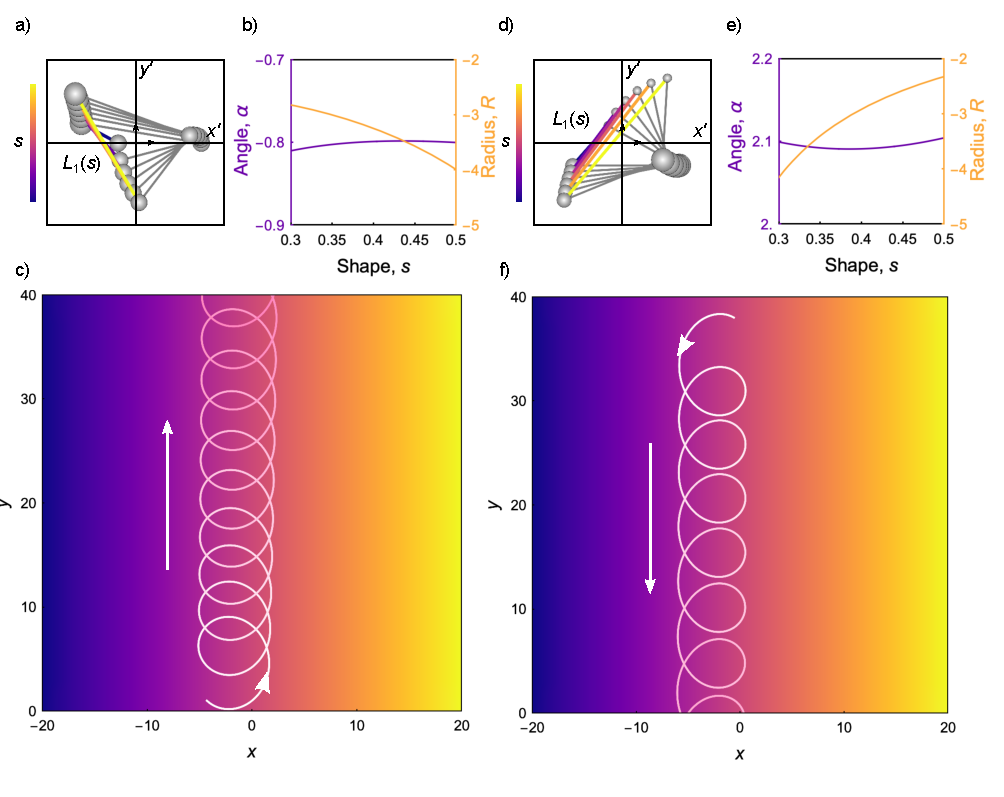
\includegraphics[width=15cm]{figures/A3_FigureS4.pdf}
    \caption{Design of two three-sphere clusters that move perpendicular to the stimulus gradient. (a,d) Standard shapes for the optimal design for different values of the shape parameter $s=(L_1-L_{\min})/(L_{\max}-L_{\min})\in [0,1]$.
    We prescribe the lengths as $L_3=1$, $L_{\min}=0.5$, $L_{\max}=1.5$. The optimal design identified for (a) is $a_1=0.1$, $a_2=0.135$, $a_3=0.1$, and $L_2=1.410$; the optimal design for (d) is $a_1=0.0670$, $a_2=0.040$, $a_3=0.108$, and $L_2=0.767$. (b,e) Computed response functions $\alpha(s)$ and $R(s)=U(s)/\Omega(s)$ for the standard shapes in (a) and (d). (e,f) Computed particle trajectory on a uniform stimulus gradient $S(\ve{x})=Gx$ of magnitude $G=0.2$; the shape parameter is assume to vary with the local stimulus as $s = (1+ e^{-S})^{-1}$.}
    \label{fig:perpChemo}
\end{figure}



%%%%%%%%%%%%%%%%%%%%%%%%%%%%%%%%%%%%%%%%%
%%%%%%%%%%%%%%%%%%%%%%%%%%%%%%%%%%%%%%%%%
%%%%%%%%%%%%%%%%%%%%%%%%%%%%%%%%%%%%%%%%%
\clearpage
\section{Derivation of the Drift Velocity with Brownian Motion}

%%%%%%%%%%%%%%%%%%%%%%%%%%%%%%%%%%%%%%%%%
%%%%%%%%%%%%%%%%%%%%%%%%%%%%%%%%%%%%%%%%%
\subsection{Analytical Solution of a Simplified Model}

To describe the effects of Brownian motion on the shape-directed dynamics of active particles, we introduce fluctuating forces, $F_x(t)$ and $F_y(t)$, and torque, $L(t)$, to the deterministic dynamics of equations (\ref{eq:theta}), (\ref{eq:xp}), and (\ref{eq:yp}) for the particle orientation $\theta$ and position $x,y$
\begin{align}
    \dot{\theta} &= \Omega + \frac{1}{\xi_r}L(t) \label{eq:langevin1}
    \\ 
    \dot{x} &= U \cos(\theta + \alpha)  + \frac{1}{\xi}F_x(t)  
    \\ 
    \dot{y} &= U \sin(\theta + \alpha) + \frac{1}{\xi}F_y(t) \label{eq:langevin3}
\end{align}	
where $\xi_r$ and $\xi$ are friction coefficients for rotation and translation, respectively.  For simplicity, we neglect any frictional coupling between the three degrees of freedom.  The fluctuating forces and torque have zero mean and satisfy the fluctuation-dissipation relation
\begin{gather}
    \langle F_x(t) \rangle = 0 \quad \text{and} \quad \langle F_x(t)F_x(t') \rangle = 2\xi k_B T\delta(t,t')
    \\
    \langle F_y(t) \rangle = 0 \quad \text{and} \quad \langle F_y(t)F_y(t') \rangle = 2\xi k_B T\delta(t,t')
    \\
    \langle L(t) \rangle = 0 \quad \text{and} \quad \langle L(t)L(t') \rangle = 2\xi_r k_B T\delta(t,t')
\end{gather}
where $k_B T$ is the thermal energy.  These overdamped Langevin equations are more conveniently described by the corresponding Fokker-Planck equation for the distribution function $f(x,y,\theta,t)$
\begin{equation}
    \frac{\partial f}{\partial t} + \frac{\partial}{\partial \theta}(\Omega f) + \frac{\partial}{\partial x}\left[ U \cos(\theta+\alpha)f\right] + \frac{\partial}{\partial y}\left[ U \sin(\theta+\alpha)f\right] =  \frac{k_B T}{\xi_r}\frac{\partial^2f}{\partial \theta^2} + \frac{k_B T}{\xi} \left(\frac{\partial^2 f}{\partial x^2}+ \frac{\partial^2 f}{\partial y^2}\right)
\end{equation}

We consider the motion of a particle with the simple response functions, $U(S)=U$, $\Omega(S)=\Omega$, and  $\alpha(S)=S$, on a uniform stimulus gradient, $S=G x$, of magnitude $G$. For this problem, we can neglect variations in $y$ such that $f(x,y,\theta,t)=f(x,\theta,t)$.  Scaling lengths by $R=U/\Omega$ and time by $\Omega^{-1}$, the Fokker-Planck equation simplifies as
\begin{equation}
    \frac{\partial f}{\partial t} + \frac{\partial f}{\partial \theta} + \frac{\partial}{\partial x}\left[\cos(\theta+Gx)f\right] =  \frac{1}{\text{Pe}_r}\frac{\partial^2f}{\partial \theta^2} + \frac{1}{\text{Pe}}\frac{\partial^2 f}{\partial x^2}
\end{equation}
where $\text{Pe}_r = \Omega \xi_r/k_B T$ and $\text{Pe}=U R \xi/k_B T$ are P\'eclet numbers for rotation and translation, respectively.  This equation admits periodic solutions on the domain $0<\theta<2\pi$ and $0<x<2\pi/G$. At long times, the distribution function approaches the following solution valid for weak gradients
\begin{equation}
    f(x,\theta) \propto \frac{1 + \text{Pe}_r^2}{G\text{Pe}_r} - \text{Pe}_r \cos (\theta + G x) + \sin (\theta + G x) + \mathcal{O}(G)
\end{equation}
From this result, the drift velocity in the $x$ direction can be evaluated as 
\begin{equation}
    V = \frac{\int_0^{2\pi} \cos(\theta+G x)f(x,\theta) d\theta}{\int_0^{2\pi} f(x,\theta) d\theta} = -\frac{G \text{Pe}_r^2}{2 (1 + \text{Pe}_r^2)}  + \mathcal{O}(G^2)
\end{equation}
For high P\'eclet number ($\text{Pe}_r\gg1$), this result is identical to that of equation (\ref{eq:xdrift2}).  For low P\'eclet number ($\text{Pe}_r\ll 1$), the drift velocity scales as $V\sim -\tfrac{1}{2}G\text{Pe}_r^2$.

%%%%%%%%%%%%%%%%%%%%%%%%%%%%%%%%%%%%%%%%%
%%%%%%%%%%%%%%%%%%%%%%%%%%%%%%%%%%%%%%%%%
\subsection{Numerical Solution of the Langevin Equation}

To simulate particle motions with arbitrary response functions and stimulus landscapes, we also implemented numerical simulations of the following Langevin equation for translational and rotational motion,
\begin{equation}
    \ve{m}\cdot \frac{d\ve{\mathcal{U}}}{d t} = \ve{\mathcal{F}}_A + \ve{\mathcal{F}}_H + \ve{\mathcal{F}}_B \label{eq:langevin}
\end{equation}
where $\ve{m}$ is a generalized mass/moment-of-inertia tensor, $\ve{\mathcal{U}} = (\ve{U}, \ve{\Omega})$ is the particle translational/rotational velocity vector, $\ve{\mathcal{F}}_A =(\ve{F}_A, \ve{L}_A)$ is the activity induced force/torque vector, $\ve{\mathcal{F}}_H$ is the hydrodynamic force/torque vector, and $\ve{\mathcal{F}}_B$ is the stochastic force/torque that gives rise to Brownian motion.\autocite{Brady1988a}  At low Reynolds numbers, the hydrodynamic force on the particle is linearly related to its velocity as $\ve{\mathcal{F}}_H = -\ve{\mathcal{R}} \cdot\ve{\mathcal{U}}$, where $\ve{\mathcal{R}}$ is the hydrodynamic resistance tensor. Consistent with equations (\ref{eq:motion1}) and (\ref{eq:motion2}) for the self-phoretic velocity, the activity induced force is equal and opposite to the hydrodynamic force, $\ve{\mathcal{F}}_A = -\ve{\mathcal{F}}_H$. The stochastic force/torque $\ve{\mathcal{F}}_B$ arises from thermal fluctuations and is characterized by
\begin{equation}
    \langle \ve{\mathcal{F}}_B \rangle =0 \quad  \text{and} \quad \langle \ve{\mathcal{F}}_B(0)\ve{\mathcal{F}}_B(t)\rangle = 2 k_B T \ve{\mathcal{R}} \delta(t)
\end{equation}
where $k_B T$ is the thermal energy, the angle brackets denote an ensemble average, and $\delta(t)$ denotes the delta function.  In contrast to the simplified model of equations (\ref{eq:langevin1})-(\ref{eq:langevin3}), this formulation accounts for the shape-dependent coupling between particle translation and rotation, which arise due to non-zero off-diagonal elements in the resistance tensor $\ve{\mathcal{R}}$. The Langevin equation (\ref{eq:langevin}) was integrated numerically in the overdamped regime, using Fixman’s midpoint scheme with a constant time step of $\Delta t = 500$ (in units of $L D/\mu A$), which is small relative to the time $L/U\sim 10^4$ based on the computed velocity.\autocite{delmotte2015simulating,Delong2015}  Figure \ref{fig:noise} illustrates two stochastic particle trajectories showing particle chemotaxis in the presence of Brownian motion.

\begin{figure}[h]
    \centering
    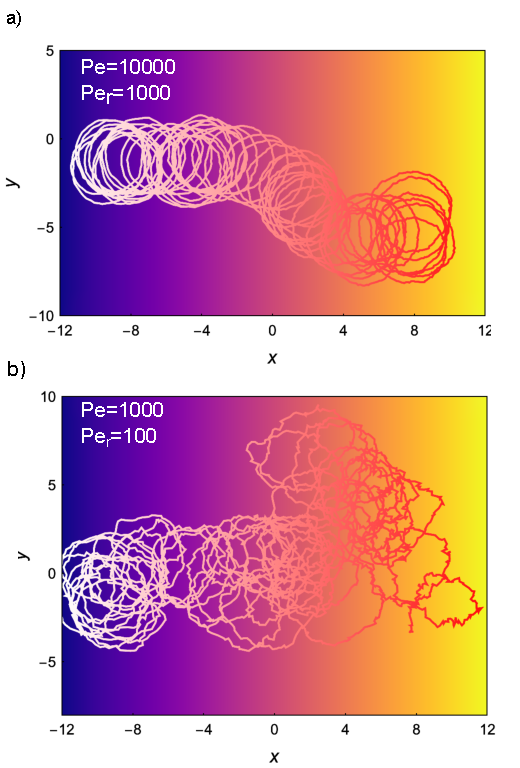
\includegraphics{figures/A3_FigureS5.pdf}
    \caption{Noisy trajectories on a uniform stimulus gradient $S(\ve{x})=Gx$ of magnitude $G=0.2$ for particles with the same geometry and shape-shifting response as those in Figure 3 of the main text: sphere radii $a_1=0.1$, $a_2=0.0985$, and $a_3=0.0958$; bond lengths $L_1\in[0.5,1.5]$, $L_2=0.677$, $L_3=1$. The magnitude of the noise is characterized by the rotational P\'eclet number, $\text{Pe}_r = \Omega \xi_r/k_B T$, using the computed value of $\xi_r$ for $s=0.5$.  The shape parameter is assume to vary with the local stimulus as $s = (1+ e^{-S})^{-1}$.}
    \label{fig:noise}
\end{figure}


                     
                  




\end{appendices}
%%%%%%%%%%%%%%%%%%%%%%%%
\begin{appendices}

%Some Table of Contents entry formatting
\addtocontents{toc}{\protect\renewcommand{\protect\cftchappresnum}{\appendixname\space}}
\addtocontents{toc}{\protect\renewcommand{\protect\cftchapnumwidth}{6em}}

%Begin individual appendices, separated as chapters

\chapter{Supplemental material for chapter 5}

%%%END OF MAIN TEXT%%%

%%%%%%%%%%%%%%%%%%%%%%%%%%%%%%%%%%
%%%%%%%%%%%%%%%%%%%%%%%%%%%%%%%%%%
%%%%%%%%%%%%%%%%%%%%%%%%%%%%%%%%%%
\section{ Perturbation Solution}

We write the governing equations (\ref{eq:theta}) and (\ref{eq:psi}) for the Euler angles $\theta(t)$ and $\psi(t)$ as 
\begin{align}
    d_t\theta &= \partial_{\tau}  \theta + \omega \partial_T = f(\theta,\psi)
    \\
    d_t\psi &= \partial_{\tau} \psi +\omega \partial_T \psi = g(\theta,\psi)
\end{align}
Substituting the expansions (\ref{eq:thetaPower}) and (\ref{eq:psiPower}), we collect like powers in $\omega$ and solve the hierarchy of perturbation equations to derive the components of the particle velocity (\ref{eq:averageU}) presented in the main text.

%%%%%%%%%%%%%%%%%%%%%%%%%%%%%%%%%%
%%%%%%%%%%%%%%%%%%%%%%%%%%%%%%%%%%
\subsubsection{Zeroth Order, $O(\omega^0)$}

The zeroth order equations are 
\begin{align}
    \partial_{\tau} \theta_0 = f(\theta_0,\psi_0)
    \\
    \partial_{\tau} \psi_0 = g(\theta_0,\psi_0)
\end{align}
On time scales of order unity, the time derivatives relax to zero, and the orientation of the particle is specified by the applied field. The resulting solution is 
\begin{align}
    \theta_0(\infty,T) &= \mathrm{atan2}((B_x^2+B_y^2)^{1/2},B_z) \label{eq:theta0}
    \\
    \psi_0(\infty,T) &= \mathrm{atan2}(B_x,-B_y) \label{eq:psi0}
\end{align}
where $\mathrm{atan2}(y,x)$ is the 2-argument arctangent function. Note that the components of the applied field depend on the slow time---for example, $B_x = B_x(T)$.

%%%%%%%%%%%%%%%%%%%%%%%%%%%%%%%%%%
%%%%%%%%%%%%%%%%%%%%%%%%%%%%%%%%%%
\subsubsection{First Order, $O(\omega^1)$}

The first order equations are 
\begin{align}
    \partial_T \theta_0 + \partial_{\tau} \theta_1 &= \theta_1 \partial_{\theta} f(\theta_0,\psi_0) + \psi_1 \partial_{\psi} f(\theta_0,\psi_0)
    \\
    \partial_T \psi_0 + \partial_{\tau} \psi_1 &= \theta_1 \partial_{\theta} g(\theta_0,\psi_0) + \psi_1 \partial_{\psi} g(\theta_0,\psi_0)
\end{align}
Substituting the zeroth order solution (\ref{eq:theta0}) and (\ref{eq:psi0}), we find the following solution for the first order quantities as $\tau\rightarrow \infty$ 
\begin{align}
    \theta_1(\infty,T) &= \frac{B_{xy} \dot{B}_z -( B_x \dot{B}_x + B_y \dot{B}_y)B_z}{B_{xy}B^3 } \label{eq:theta1}
    \\
    \psi_1(\infty,T) & = \frac{B(B_y \dot{B}_x - B_x \dot{B}_y)}{B_{xy}^2(\lambda B_{xy}^2 + B_z^2)} \label{eq:psi1}
\end{align}
where $B=(B_x^2+B_y^2+B_z^2)^{1/2}$ is the field magnitude, $B_{xy}=(B_x^2+B_y^2)^{1/2}$ is the magnitude of the field projected onto the $xy$ plane, and the dots denote derivatives with respect to the slow time.  Using these expressions, the first order contribution to the particle velocity in the $x$ direction is 
\begin{equation}
%    U_x^{(1)}(T) = \frac{B_y B_z}{B}\psi_1 - \frac{B_x B}{B_{xy}} \theta_1
    U_x^{(1)}(T) = \kappa  \left(\frac{(B_z \dot{B}_x - B_x \dot{B}_z)}{B^2} +  (\lambda-1)\frac{B_y B_z (B_x \dot{B}_y - B_y \dot{B}_x)}{B^2(\lambda B^2_{xy} + B_z^2)} \right) \label{eq:Ux1}
\end{equation}
The velocity in the $y$ direction can be obtained by permuting the $x$ and $y$ indices.

%%%%%%%%%%%%%%%%%%%%%%%%%%%%%%%%%%
%%%%%%%%%%%%%%%%%%%%%%%%%%%%%%%%%%
\subsubsection{Second Order, $O(\omega^2)$}

The second order equations are 
\begin{align}
    \partial_T \theta_1 + \partial_{\tau} \theta_2 &= -B \theta_2 - \frac{B_z B_{xy}}{2B}\psi_1^2
    \\
    \partial_T \psi_1 + \partial_{\tau} \psi_2 &=  -\frac{\lambda B_{xy}^2 + B_z^2}{B} \psi _2 - \frac{B_z (B^2 - (\lambda-1)B_{xy}^2)}{B_{xy} B}  \theta_1 \psi_1 
\end{align}
In the limit as $\tau\rightarrow\infty$, the second order solutions can be expressed in terms of the first order solutions (\ref{eq:theta1}) and (\ref{eq:psi1}) as 
\begin{align}
    \theta_2(\infty,T) &= - \frac{1}{B}\partial_T \theta_1 - \frac{B_z B_{xy}}{2 B^2} \psi_1^2 \label{eq:theta2}
    \\
    \psi_2(\infty,T) &= - \frac{B }{\lambda B_{xy}^2 + B_z^2} \partial_T \psi_1 - \frac{B_z (B^2 - (\lambda-1)B_{xy}^2)}{B_{xy} (\lambda B_{xy}^2 + B_z^2)}  \theta_1 \psi_1  \label{eq:psi2}
\end{align}
The second order contribution to the particle velocity in the $x$ direction is 
\begin{equation}
    U_x^{(2)}(T) = \kappa  \left(\frac{B_y B_z}{B}\psi_2 - \frac{B B_x}{B_{xy}} \theta_2 + \frac{B_x B_z}{2 B}\psi_1^2 + \frac{B_y B_z^2}{B B_{xy}}\theta_1 \psi_1 \right)
\end{equation}
where $\theta_2$ and $\psi_2$ are given by equations (\ref{eq:theta2}) and (\ref{eq:psi2}), $\theta_1$ and $\psi_1$ by equations (\ref{eq:theta1}) and (\ref{eq:psi1}). The velocity in the $y$ direction can be obtained by permuting the $x$ and $y$ indices.

%%%%%%%%%%%%%%%%%%%%%%%%%%%%%%%%%%
%%%%%%%%%%%%%%%%%%%%%%%%%%%%%%%%%%
%%%%%%%%%%%%%%%%%%%%%%%%%%%%%%%%%%
\section{Rotational Symmetry}

%%%%%%%%%%%%%%%%%%%%%%%%%%%%%%%%%%
%%%%%%%%%%%%%%%%%%%%%%%%%%%%%%%%%%
\subsubsection{Zeroth Order, $O(\alpha^0)$}

For fields $\ve{B}'(T)$ with rotational symmetry satisfying equation (\ref{eq:rotation}), the average velocity $\langle\ve{U}_{10}\rangle$ is identically zero as stated in equation (\ref{eq:alpha0}). To show this, we first note that an integral over one period of a periodic function is invariant to a shift in phase 
\begin{equation}
    \langle\ve{U}_{10}\rangle = \frac{1}{2\pi}\int_0^{2\pi} \ve{U}_{10}(\ve{B}'(T-\varphi_m)) dT
\end{equation}
where $\varphi_m=2\pi/m$. Using equation (\ref{eq:rotation}) for rotational symmetry, we can write the average velocity as 
\begin{equation}
    \langle\ve{U}_{10}\rangle = \frac{1}{2\pi}\int_0^{2\pi} \ve{U}_{10}(R_3(\varphi_m)\ve{B}'(T)) dT
\end{equation}
Similar equations hold for other integer multiples of the angle $\varphi_m$.  By averaging over the first $m$ multiples, we can write 
\begin{equation}
    \langle\ve{U}_{10}\rangle = \frac{1}{2\pi}\int_0^{2\pi} \left[\frac{1}{m} \sum_{n=0}^{m-1} \ve{U}_{10}(R_z(n \varphi_m)\ve{B}'(T)) \right] dT = 0 \label{eq:trick}
\end{equation}
where the integrand is identically zero. Note that the instantaneous velocity $\ve{U}_{10}$ is given by equation (\ref{eq:Ux1}) since $\ve{B}'(T)=\ve{B}(T)$ at zeroth order in $\alpha$. Using the same arguments, it can be show that the average velocity $\langle\ve{U}_{20}\rangle$ is also zero as stated in equation (\ref{eq:alpha0}).


%%%%%%%%%%%%%%%%%%%%%%%%%%%%%%%%%%
%%%%%%%%%%%%%%%%%%%%%%%%%%%%%%%%%%
\subsubsection{First Order, $O(\alpha^1)$}

For fields $\ve{B}'(T)$ with rotational symmetry satisfying equation (\ref{eq:rotation}), the average velocity $\langle U_y^{(11)}\rangle$ parallel to the gradient direction is identically zero as implied by equation (\ref{eq:alpha1}). To show this, we use the rotational symmetry of the field to simplify the integrand as in equation (\ref{eq:trick}) above 
\begin{equation}
    \langle U_y^{(11)}\rangle = \frac{1}{2\pi}\int_0^{2\pi} \left[\frac{1}{m} \sum_{n=0}^{m-1} U_y^{(10)}(R_z(n \varphi_m)\ve{B}'(T)) \right] dT
\end{equation}
The resulting integral can then be simplified as 
\begin{equation}
    \langle U_y^{(11)}\rangle = \frac{\kappa}{8\pi}\int_0^{2\pi} \frac{d}{d T}  \ln \left(\frac{2 (\lambda -1) {B'_{xy}}^2}{{B'}^2}+2 \right) dT = 0
\end{equation}
where the second equality follows from the periodicity of the field.  By contrast, the average velocity in the $x$-direction (perpendicular to the gradient) is non-zero 
\begin{equation}
    \langle U_x^{(11)}\rangle =\kappa \int_0^{2\pi} \frac{ (  \lambda(\lambda +1) {B_{xy}'}^2 + (3 \lambda -1) {B'_z}^2)(B'_x \dot{B}'_y - B'_y \dot{B}'_x)}{4\pi (\lambda  {B'_{xy}}^2 +{B'_z}^2)^2} dT \label{eq:Ux11}
\end{equation}
where the integrand has been simplified using the rotational symmetry of the field.
\end{appendices}
%


\begin{appendices}

%Some Table of Contents entry formatting
\addtocontents{toc}{\protect\renewcommand{\protect\cftchappresnum}{\appendixname\space}}
\addtocontents{toc}{\protect\renewcommand{\protect\cftchapnumwidth}{6em}}

%Begin individual appendices, separated as chapters

\chapter{Thermodynamic costs of dynamic function in active soft matter}




\section{Introduction}

Living matter performs a remarkable variety of complex functions (Fig.~\ref{fig:1}a): chloroplasts within plants capture energy from sunlight and convert it into chemical fuels and structural materials; muscle tissue powers organisms to move and to transport matter throughout their interiors; the cytoskeleton incessantly reconfigures its structural components, enabling cells to adapt their mechanical properties to their environment; the skin of vertebrate organisms provides a protective barrier that repairs itself when damaged and maintains its function despite wear; nervous tissue uses complex signaling networks to sense environmental inputs and compute intelligent outputs.  Perhaps most remarkably, all organisms grow and replicate these living materials to escape the unrelenting pull toward thermodynamic equilibrium (i.e., death). These functions---and the many others not listed---would be highly desirable to achieve in synthetic material systems, and yet we remain far from this goal. Why?

%%%%%%%%%%%%%%%%%%%%%%%%%%
\begin{figure}[!p]
     \centering
     \includegraphics[width= 8.5 cm]{figures/A5_Figure1.pdf}
     \caption{(a) Examples of dynamic functions in living matter. Left to right, top to bottom: chloroplasts, skeletal muscle, cell cytoskeleton, rhinoceros skin, neuronal network, bacterial colony. (b) Dynamic functions require the coupling of complex structures and dissipative processes---here, a kinesin motor protein bound to a microtubule does work powered by ATP hydrolysis. All images are public domain. }
%Figure source left to right , up to bottom
%https://en.wikipedia.org/wiki/Chlorophyll
%https://en.wikipedia.org/wiki/Muscle
%https://www.cshlpress.com/default.tpl?cart=1537454398711019648&fromlink=T&linkaction=full&linksortby=oop_title&--eqSKUdatarq=1107
%https://en.wikipedia.org/wiki/Rhinoceros
%https://www.flickr.com/photos/gehealthcare/4253587827/
     \label{fig:1}
 \end{figure}
%%%%%%%%%%%%%%%%%%%%%%%%%%

Materials science has traditionally focused on controlling structure and composition as the primary route to achieving function in materials. In this paradigm, material function (e.g., mechanical strength or electrical conductivity) is determined by the spatial organization of material components (e.g., atoms, molecules, nanoparticles, etc.). This approach has been widely successful. We can now create materials with heterogeneous structure and composition on length scales spanning molecular to macroscopic dimensions (e.g., an integrated circuit).  These structures form the material basis for the modern world. However, control over structure alone is insufficient to realize the \emph{dynamic functions} characteristic of living matter.

In addition to structural complexity, living matter is further distinguished by the presence of dissipative \emph{processes} that organize and animate material components in space and time to achieve dynamic function. For example, the complex structure of a kinesin motor protein is unrivaled by that of synthetic macromolecules; however, its ability to perform mechanical work requires energy input and temporal control provided by chemical reactions (Fig.~\ref{fig:1}b). More generally, the dynamic functions of living matter require integration of structures \emph{and} processes to drive material organization in space and time.  Such organization is not possible at thermodynamic equilibrium but instead requires flows of energy and matter to create and maintain spatiotemporal order among the system's components.  These currents dissipate energy as heat and waste, thereby increasing the entropy of the surroundings.  In short, dynamic functions have a thermodynamic cost: living matter needs to eat. 

The creation of synthetic material systems that perform dynamic functions requires a different paradigm---one in which material structures are coupled to and animated by networks of dissipative processes.  Progress towards this challenging goal is underway in a variety of fields.  In statistical physics, interest in non-equilibrium thermodynamics \cite{de2013non} has been renewed by the discovery of non-equilibrium principles---such as fluctuation theorems \cite{jarzynski2011equalities} and uncertainty relations \cite{Seifert2018}---that describe the behavior of small (fluctuating) systems driven away from equilibrium \cite{Seifert2012,Marsland2018}.  These principles are being applied to elucidate the biophysical mechanisms of cellular oscillators \cite{Cao2015,Barato2016}, molecular motors \cite{Pietzonka2016,Hess2017}, dissipative assemblies \cite{Nguyen2015, marsland2018active}, and sensory adaptation \cite{Lan2012,Tu2018} among others.  The study of active matter \cite{Marchetti2013} shifts the focus from individual driven components such as molecular motors to their large scale collective behaviors \cite{Needleman2017, Doostmohammadi2018}. The creation of self-propelled particles---so-called active colloids \cite{Bechinger2016, illien2017fuelled, Zhang2017}---provides synthetic realizations of active matter with emerging opportunities as autonomous microrobots \cite{Palagi2018, han2018engineering}. The chemical synthesis of molecular motors \cite{kassem2017artificial,Astumian2017} and dissipative assemblies \cite{VanRossum2017,De2018} highlight the potential for systems chemistry \cite{Ashkenasy2017}, in which molecular systems are guided by dissipative networks of chemical reactions \cite{Epstein2016, Grzybowski2017}. Inspired by living matter, these diverse pursuits promise advances in molecular systems \cite{merindol2017materials}, nanotechnology \cite{Grzybowski2016},  biomaterials \cite{tibbitt2017living}, and even artificial cells \cite{Yewdall2018}.

Here, we integrate elements from these different fields to provide an idiosyncratic perspective on the creation of \emph{active soft matter}. This label refers to systems of molecules, polymers, and particles in liquid environments that move and interact with characteristic energies comparable to the thermal energy at room temperature. Moreover, these materials are driven and maintained away from equilibrium by external thermodynamic forces, resulting in flows of matter and energy needed to perform dynamic functions. This broad definition, encompassing much of cell biology, active matter, and systems chemistry, is united by a common framework---that of, \emph{stochastic thermodynamics} \cite{Seifert2012}---which describes small driven systems immersed in a heat bath.  The dynamics of such systems are described by stochastic processes, in which the concepts of work, heat, and entropy production are described at the level of fluctuating trajectories. Even far from equilibrium, these fluctuating quantities obey universal relations, which establish fundamental trade-offs between the rate of energy dissipation and performance metrics such as precision, efficiency, and speed. 

In pursuit of active soft matter, we advocate a constructionist perspective summarized by Richard Feynman: ``What I cannot create, I do not understand.'' If we seek to understand the inner workings of living matter, we should strive to create synthetic analogs---perhaps greatly simplified---that perform similar dynamic functions. These analogs or ``models'' can be material or conceptual---for example, a synthetic molecular motor or a mathematical description thereof.  In both cases, the construction of the model, marked by false starts and dead ends, teaches us what is necessary and what is superfluous to achieving the targeted function.  Moreover, by building systems that push the limits of performance, we discover universal bounds that constrain the operation of biological and non-biological matter alike.

The constructionist approach should be directed and motivated by the pursuit of dynamic function to avoid the creation of models for their own sake without generating broader insights.  Living matter dissipates energy to perform remarkable functions; however, dissipation alone is unremarkable. The Reader would not be impressed by a ``life-like'' paper weight that requires a steady supply chemical fuel for its operation. Many functions---like keeping documents in order---can and should be achieved without dissipating energy. Instead of focusing on dissipation as a hallmark of living matter, we should shift our attention to the dynamic functions we aim to achieve.  How can we make a chemical clock that oscillates more reliably?  How can we convert chemical energy to mechanical work more efficiently?  How can we assemble and disassemble material structures more quickly?  The pursuit of these and other dynamic functions in active soft matter can serve to orient and guide our exploration of this exciting new field.

In this spirit, the present Review is organized around four dynamic functions under the headings of (1) keeping time, (2) powering motion, (3) building structures, and (4) making copies. For each function, we present a simple kinetic model that identifies the essential ingredients and illustrates the fundamental trade-offs between dissipation and performance. These examples are often adapted from biophysical models and repackaged in the context of synthetic materials such as colloidal machines, nanoparticle assemblies, and DNA nanotechnology. In this way, the complex functions of biology are simplified into minimal models, which in turn guide the design of bioinspired, synthetic materials. Building on general lessons from the models, we discuss recent progress and challenges in creating active soft matter capable of dynamic functions. Our coverage of the recent literature is far from comprehensive. Instead, we aim to bridge experimental efforts in active soft matter and theoretical advances from stochastic thermodynamics to inform future research on material systems inspired by living matter. To this end, we begin with a brief introduction to the stochastic thermodynamics of non-equilibrium steady-states and the thermodynamic uncertainty relation  \cite{Barato2015, Gingrich2016, Pietzonka2016b}. It is our hope that this cross-disciplinary perspective will spark new connections among communities interested in understanding, designing, and constructing dissipative material systems.

%%%%%%%%%%%%%%%%%%%%%%%%%%
%%%%%%%%%%%%%%%%%%%%%%%%%%
\section{Stochastic Thermodynamics}

The kinetic models presented below are described by the framework of stochastic thermodynamics, which considers the fluctuations of thermodynamic quantities in small systems driven out of equilibrium by external forces \cite{Seifert2012, VanDenBroeck2015, Ciliberto2017} (see \cite{Seifert2018} for a recent and accessible introduction to the field).  Here, we briefly summarize the concepts relevant to our discussion of dynamic function. We consider systems at constant temperature maintained in non-equilibrium steady-states by chemical reactions or other thermodynamic forces.  Our choice to exclude phenomena involving time-varying fields \cite{Barato2016,Barato2017b} or thermal gradients \cite{Pietzonka2018} is one of convenience and should not be viewed as a limitation of stochastic thermodynamics.  Systems at steady-state obey a universal non-equilibrium principle known as the thermodynamic uncertainty relation \cite{Barato2015, Gingrich2016, Pietzonka2016b}, which bounds the magnitude of current fluctuations by the rate of entropy production.  This recent advance in non-equilibrium statistical mechanics has important implications for the performance of small machines and therefore the design of active soft matter.

%%%%%%%%%%%%%%%%%%%%%%%%%%
\subsection{Markovian Networks}

We consider a coarse-grained description of the system in which the many microstates are partitioned into $N$ mesostates, each characterized by an equilibrium free energy $F_i$ for $i=1\dots N$.  The validity of this description relies on the separation of time scales for transitions within each mesostate (fast) and between different mesostates (slow).  At equilibrium, the probability of finding the system in the $i^{\text{th}}$ mesostate (henceforth ``state'') is given by the Boltzmann distribution, $p_i \propto \exp(-F_i)$. For notational convenience, we have set Boltzmann constant $k_B$ and the temperature $T$ to unity, such that all energies are given in units of the thermal energy $k_B T$.  At equilibrium, there are no net currents between any two states: the current $k_{ij} p_i$ from state $i$ to $j$ is equal to the current $k_{ji} p_j$ from state $j$ to $i$.  This condition of detailed balance implies that the transition rates $k_{ij}$ and $k_{ji}$ are related  at equilibrium as $\ln(k_{ij}/k_{ij})=F_i-F_j$. 

In driven systems, the application of thermodynamic forces---also called affinities---result in steady currents through the network of states.  A network of $N$ states connected by $E$ edges with non-zero transition rates ($k_{ij}\neq 0$) has $E-N+1$ independent currents, one for each fundamental cycle of the network \cite{schnakenberg1976network}.  The fluctuating current $X_{\beta}(t)$ around the cycle $\beta$ counts the number of cycle completions, increasing or decreasing by 1 on completion of the forward or reverse cycle, respectively.  In addition to the integrated current $X_{\beta}(t)$, the average current $J_{\beta}$ measures the number of cycle completions per unit time,
\begin{equation}
    J_{\beta} \equiv \langle X_{\beta}(t)\rangle / t
\end{equation}
where the brackets indicate an average over stochastic trajectories at steady-state.  Alternatively, the average current can be computed from the steady-state occupancy probabilities $p_i$ as $J_{\beta} = k_{ij} p_i - k_{ji} p_j$, where the edge $ij$ corresponds to a particular transition used in defining the set of fundamental cycles (see \cite{schnakenberg1976network} for details).  As at equilibrium, the occupancy probabilities at steady-state are defined by the set of linear equations, $k_{ij} p_i = k_{ji} p_j$.

The thermodynamic affinity $\mathcal{A}_{\beta}$ driving the cycle currents describes the decrease in free energy of the surroundings upon completion of the cycle $\beta$.  For example, the affinity of a cycle that consumes one ATP molecule and produces one ADP molecule is equal to the difference in chemical potentials of ATP and ADP in the surrounding reservoirs, $\mathcal{A}_{\beta}=\mu_{\text{ATP}}-\mu_{\text{ADP}}$.  In general, a single cycle may be associated with multiple processes (e.g., chemical reactions, mechanical motions) that contribute to its overall affinity $\mathcal{A}_{\beta}$.  To account for this possibility, we introduce a generalized distance $d^{\beta}_{ij}$ that describes the fraction of the cycle affinity $\mathcal{A}_{\beta}$ associated with the particular transition $i\rightarrow j$.  Considering both the system and its surroundings, the condition of detailed balance implies the following relation between the forward and reverse transition rates
\begin{equation}
    \ln\left(\frac{k_{ij}}{k_{ji}}\right) = \sum_{\beta} d^{\beta}_{ij} \mathcal{A}_{\beta} + F_i - F_j 
\end{equation}
During the transition $i\rightarrow j$, the fluctuating current $X_{\beta}(t)$ increases by the generalized distance $d^{\beta}_{ij}$; the fluctuating entropy change in the surrounding medium $s_m(t)$ increases by the increment $d^s_{ij} = \ln(k_{ij}/k_{ji})$.  The average rate of entropy production $\sigma$ is defined as 
\begin{equation}
    \sigma \equiv\langle s_m(t)\rangle / t = \sum_{\beta}\mathcal{A}_{\beta} J_{\beta} \label{eq:entropy}
\end{equation}
which is positive for non-equilibrium steady-states and zero at equilibrium.  For the isothermal systems considered here, the rate of entropy production is equivalent to the rate of energy dissipation.  We use these terms interchangeably in our discussion of the thermodynamic cost of dynamic functions.  

%%%%%%%%%%%%%%%%%%%%%%%%%%
\subsection{Thermodynamic Uncertainty Relation}

At the non-equilibrium steady-state, general results regarding the magnitude of fluctuations can be derived using techniques from large-deviation theory \cite{Touchette2009}. In particular, the thermodynamic uncertainty relation \cite{Barato2015,Gingrich2016} provides a universal bound on rate of dissipation required to achieve a desired level of precision in the fluctuating current $X_{\beta}(t)$. The precision is characterized by the scaled variance of the current $X_{\beta}(t)$, which provides a measure of uncertainty for the cyclic process,
\begin{equation}
    \epsilon^2_{\beta} \equiv \frac{\langle X_{\beta}^2 \rangle -\langle X_{\beta} \rangle^2 }{\langle X_{\beta} \rangle^2} = \frac{2 D_{\beta}}{J^2_{\beta} t}
\end{equation}
Here, $D_{\beta}\equiv ( \langle X_{\beta}^2 \rangle -\langle X_{\beta} \rangle^2) / t$ is the dispersion of the process, which approaches a constant value in the limit of long times.  Additionally, the cost of running this process for a time $t$ is equal to the average amount of entropy produced (or energy dissipated), $\mathcal{C} = \sigma t$. The thermodynamic uncertainty relation describes the fundamental trade-off between precision and dissipation for any Markov process
\begin{equation}
     \mathcal{C}\epsilon^2_{\beta} = \frac{2\sigma D_{\beta}}{J_{\beta}^2} \geq 2 \label{eq:TUR}
\end{equation}
Achieving greater precision (smaller $\epsilon_{\beta}^2$) comes only at the expense of higher cost (larger $\mathcal{C}$).  

The uncertainty relation (\ref{eq:TUR}) is saturated near equilibrium, at which the affinities $\mathcal{A}_{\beta}$ vanish. For large affinities characterizing ``far-from-equilibrium'' processes, there exist stronger but less general bounds for networks of certain simple topologies \cite{Pietzonka2016b}.  In particular, for a single cycle with $N$ states, the uncertainty relation is bounded by the affinity-dependent inequality  
\begin{equation}
    \mathcal{C}\epsilon^2 \geq \frac{\mathcal{A}}{N}\coth\left(\frac{\mathcal{A}}{2N}\right) \geq 2 \label{eq:unicycle}
\end{equation}
As illustrated in the example below, such bounds may be tighter or looser depending on the specific transition rates characterizing the system dynamics. 

%%%%%%%%%%%%%%%%%%%%%%%%%%
\subsection{Tutorial example: An electromechanical oscillator}

To demonstrate the mechanics of building and interrogating a simple kinetic model, we consider the dynamics of an electromechanical oscillator that shuttles charge between two electrodes subject to an applied voltage $V$ (Fig.~\ref{fig:KeepingTime}a). This system has been studied previously at the microscale as an electric motor for powering unit operations in microfluidic systems \cite{bishop2018contact,drews2015contact}.  Here, we describe an analogous system at the nanoscale, in which a particle (or molecule) transitions repeatedly between two charged states, $+e$ and $-e$, where $e$ is the elementary charge.  These transitions are assumed to occur only when the particle is located near the surface of either electrode.  The system is therefore modeled by $N=4$ discrete states corresponding to the two particle locations and two particle charges (Fig.~\ref{fig:KeepingTime}a).  For simplicity, we assume that the system is symmetric such that the free energy of the positively charged particle at the negatively biased electrode (state 1) is the same as that of the negatively charged particle at the positively biased electrode (state 3).  These states (1 and 3) are lower in energy than the others (2 and 4) by a common factor $\Delta F>0$, which implies that the charged particle moves spontaneously towards the oppositely biased electrode (Fig.~\ref{fig:KeepingTime}b).

%%%%%%%%%%%%%%%%%%%%%%%%%%
\begin{figure}[p!]
    \centering
    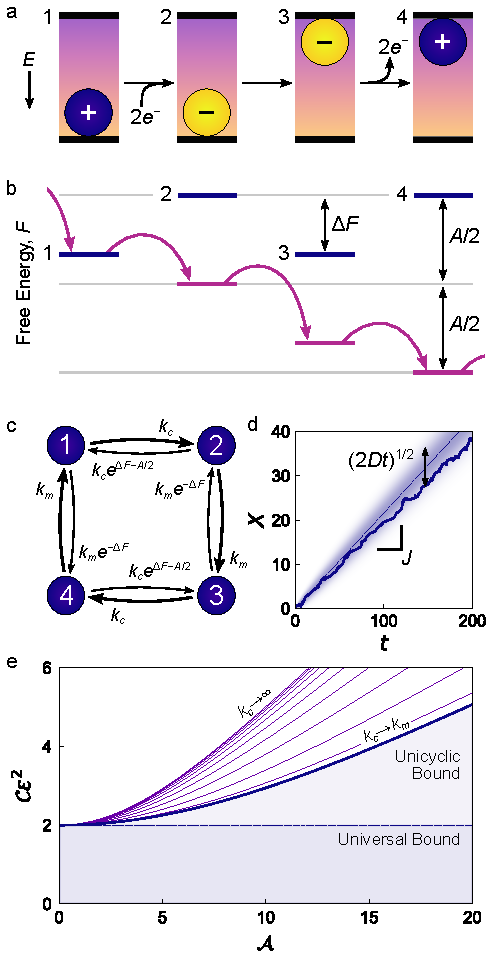
\includegraphics{figures/A5_KeepingTime.pdf}
    \caption{\textbf{Keeping Time.}(a) A 4-state Markov model of an electromechanical oscillator moving between two electrodes. (b) Free energy diagram showing the energies of the four states (blue) and the total energy of the system and its surroundings (purple). The arrows show how the total energy decreases by $\mathcal{A}$ during one cycle. (c) Markov network showing the relevant transition rates. (d) Fluctuating current $X(t)$ as a function of time for $\mathcal{A}=8$, $\Delta F=2$, and $k_c= 1$.  The shaded region shows the distribution for $X(t)$ as characterized by the average rate $J$ and dispersion $D$. (e) Computed product of the cost $\mathcal{C}$ and uncertainty $\varepsilon^2$ as a function of the affinity $\mathcal{A}$ for different values of the charging rate $k_c$ (purple curves).  The product $\mathcal{C}\epsilon$ is greater than the universal bound (\ref{eq:TUR}) and the unicyclic bound (\ref{eq:unicycle}). }
    \label{fig:KeepingTime}
\end{figure}
%%%%%%%%%%%%%%%%%%%%%%%%%%

The network is characterized by a single cycle with affinity $\mathcal{A}= 2 e V / k_B T$, corresponding to the transfer of 2 elementary charges down the potential difference $V$. The generalized distances described above are given by $d_{12}=d_{34}=1/2$ and $d_{32}=d_{41}=0$.  Transitions with $d_{ij}\neq0$ are coupled to the external reservoirs (electrodes) via charge transfer processes that allow for driving the system to higher energy states (Fig.~\ref{fig:KeepingTime}b).  Note, however, that the total energy of the system \emph{and} its environment decreases by an amount $\mathcal{A}$ during each cycle.  At steady-state, this thermodynamic force drives an average current $J$ which increases (nonlinearly) with the affinity $\mathcal{A}$.    

In addition to the network topology and energetics, the system's dynamics are determined by kinetic rate constants that reflect the speed of the different transitions. Accounting for the conditions of detailed balance and symmetry, the present model requires two such rate constants: one for charge transfer $k_c$ and another for particle motion $k_m$ (Fig.~\ref{fig:KeepingTime}c). We choose to measure time in units of $k_m^{-1}$ and thus set the rate constant $k_m$ to unity. The dynamics of the model is specified by three (dimensionless) parameters: the driving affinity $\mathcal{A}$, the free energy difference $\Delta F$, and the remaining rate constant $k_c$.  Figure \ref{fig:KeepingTime}d shows one realization of the fluctuating current $X(t)$ for $\mathcal{A}=8$, $\Delta F=2$, and $k_c= 1$.  The current increases at an average rate $J$ with dispersion $D$, which are computed analytically following the method of Koza \cite{koza1999general} (see also \cite{Pietzonka2016b}).

%%%%%%%%%%%%%%%%%%%%%%%%%%
%%%%%%%%%%%%%%%%%%%%%%%%%%
\section{Dynamic Functions}

Armed with the framework of stochastic thermodynamics, we now consider the theoretical analysis and synthetic realization of four dynamic functions in active soft matter: (1) keeping time, (2) powering motion, (3) building structures, and (4) making copies.

%%%%%%%%%%%%%%%%%%%%%%%%%%
\subsection{Keeping Time}

Biochemical oscillations are critical in controlling the timing of dynamic functions within living matter.  In particular, the different circadian rhythms allow organisms to anticipate and prepare for periodic changes in their environment such as light-dark cycles. The ability to keep accurate time enables organisms to more effectively harness environmental resources (e.g., light and food) and coordinate internal processes \cite{Sharma2003}. The benefits of ``keeping time'' come only at a thermodynamic cost \cite{Cao2015, Barato2016} in the form of energy dissipation. The thermodynamic uncertainty relation (\ref{eq:TUR}) establishes the universal trade-offs between the precision of small clocks and the energy currents required for their operation \cite{Barato2016}.  Here, we discuss these trade-offs in the context of a model Brownian clock---namely, the electromechanical oscillator introduced in the previous section.  We identify strategies for achieving optimal performance and highlight some recent progress in the design of synthetic oscillators. 

%%%%%%%%%%%%%%%%%%%%%%%%%%
\subsubsection{A Brownian Clock}

The electromechanical oscillator introduced in Figure \ref{fig:KeepingTime} provides a simple example of a Brownian clock \cite{Barato2016} where each cycle measures one ``tick'' of mean duration $J^{-1}$.  In using this clock to measure a specified time interval $\mathcal{T}$, we consider two performance metrics: the temporal precision $\epsilon^2$ and the thermodynamic cost $\mathcal{C}$.  First, an effective clock must be sufficiently precise.  For example, the timing of Olympic sprinters requires precision better than $\epsilon=10^{-3}$ to measure a 10 s interval accurate to 0.01 s.  Without this precision, the clock is useless: all sprinters finish the race in $10\pm1$ s.  The thermodynamic uncertainty relation states that temporal precision can be achieved only at a thermodynamic cost.  Here, the cost of running the clock is equal to the average amount of energy supplied to the electromechanical oscillator, $\mathcal{C}= J\mathcal{A}\mathcal{T}$.  The minimum cost of any Brownian clock is $\mathcal{C}_{\min} = 2/\epsilon^2$.  Timing the hundred meter dash requires a minimum energy input of more than $10^{6}$ times the thermal energy.

Real clocks may operate at costs substantially higher than this theoretical minimum.  Kinetic models are therefore useful in guiding improvements in system performance. One approach is reducing the driving affinity $\mathcal{A}\rightarrow 0$ to operate close to thermodynamic equilibrium (Fig.~\ref{fig:KeepingTime}e).  While thermodynamically efficient, this regime is often impractical as the speed of the clock slows to zero, $J(\mathcal{A})\rightarrow0$.  As a result, long times are required to achieve the desired precision---specifically, $\mathcal{T}=2D/J^2\epsilon^2\rightarrow\infty$ for constant $D$ and $\epsilon^2$.  In the opposite limit of large driving affinity $\mathcal{A}\gg N$, the unicyclic bound (\ref{eq:unicycle}) implies a higher minimum cost of $\mathcal{C}_{\min}=\mathcal{A}/N$.  Achieving this bound requires unicyclic networks with no ``bottlenecks'', in which all transitions occur at similar rates (Fig.~\ref{fig:KeepingTime}e). In designing cyclic processes, one should therefore focus on accelerating the slowest (rate-limiting) steps, which lead to wasteful dissipation and require higher affinities to drive the desired currents.

A single oscillating particle may be effective in keeping time, but it is less useful in broadcasting this temporal information to its surroundings. Similarly, a collection of Brownian clocks cannot be used to coordinate temporal functions throughout a common volume unless they ``tick'' in synchrony.  The synchronization of Brownian clocks requires interactions between their cyclic processes, often achieved through the diffusive exchange of participating components.  In the circadian clock of cyanobacteria, the KaiC protein progresses through a cyclic sequence of phosphorylation states powered by ATP hydrolysis \cite{Dong2008}. Importantly, however, these transitions are facilitated by the binding and unbinding of other proteins, KaiA and KaiB, which are present in solution and available for binding to any oscillator.  During each cycle, KaiC proteins both influence and respond to concentration changes within the common pool of KaiA and KaiB, thereby enabling global synchronization.  The resulting oscillations in component concentrations requires an additional cost beyond that required for oscillator precision \cite{Cao2015}.  The cost of synchronization derives from the large driving affinities necessary to produce nonlinear dynamics in the system's chemical kinetics.

%%%%%%%%%%%%%%%%%%%%%%%%%%
\subsubsection{Synthetic Oscillators}

The history of synthetic chemical clocks traces it roots to Belousov's discovery around 1950 of a cerium-based analog of the Krebs cycle---the now ubiquitous Belousov-Zhabotinsky (BZ) reaction \cite{winfree1984prehistory}. Since this time, a variety of synthetic oscillators have been developed and investigated to uncover the detailed kinetic mechanisms underlying their operation \cite{epstein1998introduction}. More recent efforts have focused on the rational design of synthetic oscillators from increasingly diverse chemical components \cite{DeKepper1981, Kurin-Csorgel2005, semenov2015rational, Semenov2016}, the control of such oscillators via external stimuli \cite{Petrov1997, pogodaev2017photochemical}, and the coupling of chemical clocks to other processes such as self-assembly \cite{Lagzi2010,tagliazucchi2014dissipative}, sensing \cite{Epstein2012}, and material actuation \cite{Yashin2012, Yoshida2014, Tamate2016}.  

The analysis of biochemical oscillators has helped to identify the key ingredients for achieving chemical oscillations: negative feedback, time delay, nonlinearity, and balanced rates \cite{Novak2008}.  The application of these principles in designing synthetic oscillators is nicely illustrated by the enzymatic oscillator of Semenov \emph{et al.}, which uses time-delayed negative feedback combined with autocatalytic regeneration of the inactive enzyme \cite{semenov2015rational} (Fig.~\ref{fig:KeepingTime2}a). Once the necessary topology of the reaction network is established, the key challenge is tuning the various rates to identify suitable conditions for oscillations. This process requires a detailed understanding of each reaction step as well as external ``knobs'' by which to control their rates---for example, the choice of proinhibitor and the species concentrations \cite{semenov2015rational}.  The way in which material is supplied to and removed from the system can also be used to guide the desired oscillatory behavior. Oscillations are often achieved using continuously stirred tank reactors (CSTRs), which provide only a crude analogy to the open system of a living cell. In the former, all components are flowed into and out of the system. By contrast, cells rely on the selective exchange of chemical fuel and waste to generate nonequilibrium conditions while retaining their internal components.  Other strategies for ``feeding'' active soft matter involve the diffusive delivery (removal) of fuel (waste) to catalytic components immobilized onto or compartmentalized within material structures \cite{zhang2014giant, Tamate2016}.

%%%%%%%%%%%%%%%%%%%%%%%%%%
\begin{figure}[h!]
    \centering
    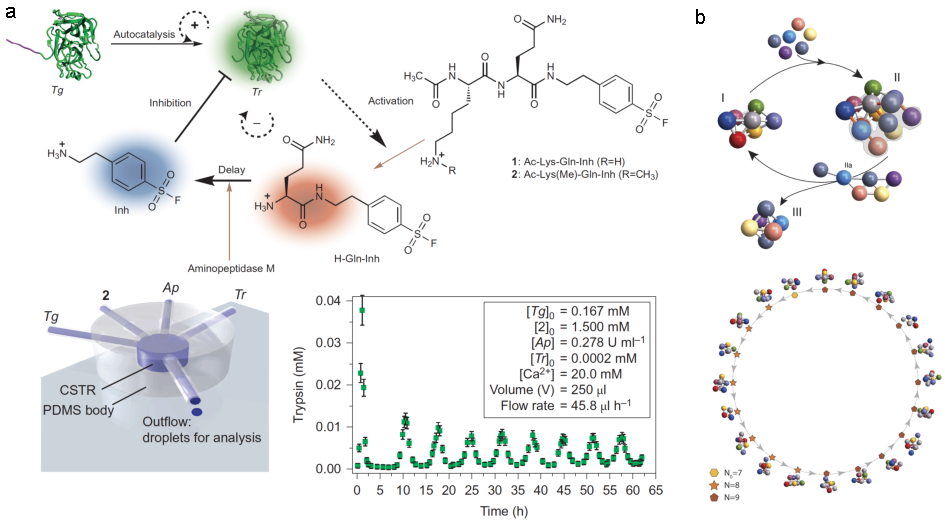
\includegraphics[width=8.5cm]{figures/A5_KeepingTime2.pdf}
    \caption{(a) Chemical reaction network for an enzymatic oscillator.  The enzyme Trypsin (Tr) catalyzes its own production from the inactive form Trypsinogen (Tg) and also the activation of its own inhibitor (Inh). Importantly, the production of the inhibitor is delayed in time, resulting in concentration oscillations of Trypsin within a continuously stirred tank reactor (CSTR). \kbnote{(Adapted from Ref.~\cite{semenov2015rational} with permission.)} (b) A seven particle cluster (I) catalyzes the formation of an octahedral cluster (III) via specific time-varying interactions (left). Such templating reactions lead to the emergence of  exponentially growing catalytic cycles within a pool of monomers (right). \kbnote{(Adapted from Ref.~\cite{Zeravcic2017} with permission.)}}
    \label{fig:KeepingTime2}
\end{figure}
%%%%%%%%%%%%%%%%%%%%%%%%%%

These and other synthetic oscillators are typically macroscopic---even femtoliter droplets of the BZ reagent contain more than 10 million copies of the oscillating redox complex \cite{Toiya2010, Tompkins2014}. Consequently, questions of oscillator precision are rarely a concern. However, as the number of oscillators decreases, the effects of thermal noise and phase diffusion are expected to grow. Can the BZ reaction or other synthetic oscillators operate coherently on the scale of nanometers \cite{Epstein2016}?  To address these and other questions of fluctuating oscillators, model systems based on colloidal particles may prove useful. Experimental studies have shown that transformations between colloidal assemblies can mimic those found in chemical reactions \cite{Meng2010, Chen2011}. By modulating their interactions in time, theoretical studies have demonstrated the emergence of catalytic cycles among small clusters of colloidal spheres (Fig.~\ref{fig:KeepingTime2}b) \cite{Zeravcic2017, zeravcic2017colloquium}. We note, however, that the precision of cyclic processes powered by time-periodic drives are not bound by the uncertainty relation \cite{Barato2016}. Colloidal systems powered by constant thermodynamic forces, such as collections of electromechanical oscillators \cite{Dou2018}, may therefore be useful in investigating the costs of precision and synchronization in small machines.

%%%%%%%%%%%%%%%%%%%%%%%%%%
\subsection{Powering Motion}

Many living organisms are capable of performing mechanical work to drive motion and transport on scales spanning the molecular to the macroscopic. In natural muscle \cite{Alberts2015}, macroscopic actuation is achieved by hierarchical assemblies of many micron-scale actuators (sarcomeres), in which myosin motors ratchet their way along actin fibers through a series of chemically powered conformation changes and binding events. Acting in concert, these molecular motors give rise to macroscopic stresses of ${\sim}0.1$ MPa, strains of ${\sim}30$\%, and strain rates of up to 500\% s$^{-1}$.  Such performance is not achieved at 100\% efficiency as permitted at constant temperature by classical thermodynamics.  Kinetic models of small machines reveal the fundamental trade-offs between efficiency, power, and fluctuations that constrain motor performance \cite{Pietzonka2016}. Here, we use the driven oscillations of our electromechanical oscillator (Fig.~\ref{fig:KeepingTime}) to perform mechanical work and discuss how motor performance is bound by the uncertainty relation (\ref{eq:TUR}).  We highlight recent efforts in synthesizing molecules and colloids that convert chemical energy into motion and discuss the outstanding challenges of emulating natural muscle.

%%%%%%%%%%%%%%%%%%%%%%%%%%
\subsubsection{An Electromechanical Ratchet}

The electromechanical oscillator described above can be harnessed to produce directed motion or perform mechanical work against an applied load. Figure \ref{fig:PoweringMotion}a shows one strategy for rectifying particle oscillations within channels flanked by an array of asymmetric barriers with period $d$. This approach has been demonstrated experimentally within microfluidic channels \cite{drews2013ratcheted}; however, the concept is also applicable at smaller scales where thermal motions become significant \cite{kowalik2016ratcheted}. The stochastic motion of the particle through the ratcheted channel can be modeled by the periodic Markov network illustrated in Figure \ref{fig:PoweringMotion}b. In the absence of an external load ($f=0$), the affinity $\mathcal{A}$ due to the applied voltage drives the particle through the following sequence of states. First, a positively charged particle transfers charge to the negatively biased electrode ($1\rightarrow2$). Now negatively charged, the particle moves in the applied field to the opposite electrode ($2\rightarrow3$). During this transition, the barrier forces the particle to move either to the right with rate $k_m$ or to the left with rate $\gamma k_m$. The geometric asymmetry of the barrier is designed to favor motion to the right such that $\gamma \ll 1$. After charge transfer at the opposite electrode ($3\rightarrow 4$), the particle again moves preferentially to the right into state 1 of the neighboring unit cell ($4\rightarrow 1^+$). Overall, the particle moves a distance $d$ during each cycle as directed by the asymmetric barriers.

%%%%%%%%%%%%%%%%%%%%%%%%%%
\begin{figure}[ht]
    \centering
    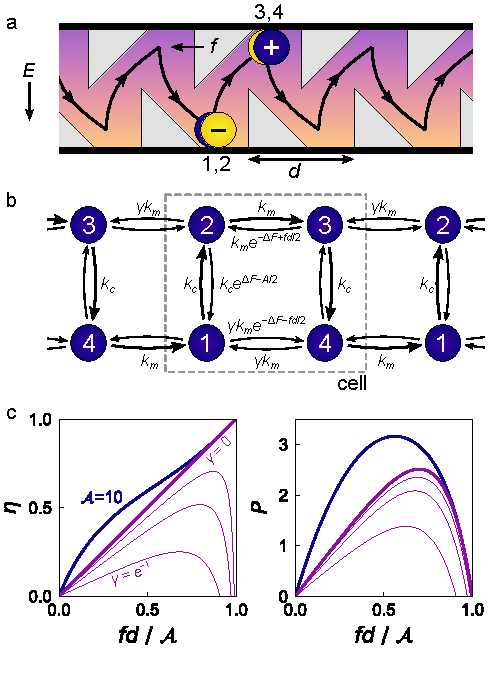
\includegraphics{figures/A5_PoweringMotion.pdf}
    \caption{\textbf{Powering Motion.} (a) Schematic illustration of an electromechanical ratchet based on the oscillator in Figure \ref{fig:KeepingTime}. (b) Markov network for the ratchet showing the transition rates within and between the unit cells. (c) Motor efficiency (left) and power (right) as a function of the applied load for an affinity of $\mathcal{A}=10$. The blue curve denotes the bound (\ref{eq:efficiency}); the purple curves shows the motor performance for $\gamma=e^{-1}, e^{-2}, e^{-3},  \text{ and } 0$.}
    \label{fig:PoweringMotion}
\end{figure}
%%%%%%%%%%%%%%%

Each of the forward transitions is accompanied by a reverse transition whose rate is determined by the detailed balance condition accounting for the free energy difference between the states $\Delta F$, the driving affinity $\mathcal{A}$, and the applied load $f$.  The fluctuating position of the particle $X(t)$ increases or decreases by an amount $d$ upon transition from one unit cell to the next. At steady-state, the average velocity, $v$, of the particle is given by 
\begin{equation}
    v = \frac{\langle X(t)\rangle}{t}= \sum_{ij} p_i (w_{ij}^+ - w_{ij}^-)d
\end{equation}
where $w_{ij}^{\pm}$ denotes the transition rate from state $i$ in the current cell to state $j$ in the cell to the right/left (e.g., $w_{41}^+=k_m$ and $w_{23}^-=\gamma k_m$). Particle motion against the applied load $f$ results in a fluctuating power output $P(t)$ with an average value of $P=fv$. At the same time, this electromechanical motor dissipates energy at an average rate $\sigma$, as specified by the principles of stochastic thermodynamics \cite{Pietzonka2016}.  With these quantities, the thermodynamic efficiency of the motor is given by the fraction of energy supplied to the system that is converted into useful work, $\eta = P / (P+\sigma)$. In addition to the average power and efficiency, the motor is further distinguished by its constancy, as characterized by power fluctuations
\begin{equation}
    \Delta_P = \lim_{t\rightarrow \infty}\langle (P(t)-P)^2 \rangle t = 2 D f^2
\end{equation}
where $D$ is the dispersion of the particle position.

These three quantities---the power $P$, efficiency $\eta$, and constancy $\Delta_P$---are constrained by the thermodynamic uncertainty relation \cite{Pietzonka2016} as 
\begin{equation}
    \eta \leq \frac{1}{1+2P/\Delta_p} \label{eq:efficiency}
\end{equation}
This universal result suggests two fundamentally different strategies for improving the efficiency of a stochastic motor.  First, one can operate near equilibrium such that the average power vanishes ($P\rightarrow0$) with finite power fluctuations (Fig.~\ref{fig:PoweringMotion}c).  Like a clock without precision, a motor without power is of little practical value regardless of its efficiency.   An alternate route to achieving maximum efficiency is increasing the power fluctuations ($\Delta_p\rightarrow\infty$) at finite power; however, large fluctuations may be unacceptable for certain applications.  In the face of competing performance criteria, the ``optimal'' motor depends on the context.

Like related models of molecular machines \cite{Pietzonka2016}, the electromechanical ratchet has a maximum efficiency of $\eta=f d/\mathcal{A}$ in the limit of perfect biasing ($\gamma\rightarrow 0$).  In this limit, the energy $\mathcal{A}$ supplied during each step contributes a fixed amount $f d$ to the total work performed.  For a driving affinity $\mathcal{A}=10$, the efficiency at maximum power is 70\% assuming fast charging ($k_c/k_m\rightarrow\infty$); the fundamental bound under these conditions is 73\% (Fig.~\ref{fig:PoweringMotion}c).  While detrimental to motor efficiency, the uneven allocation of dissipation among the different steps is often beneficial in increasing power output \cite{brown2017allocating}. 

%%%%%%%%%%%%%%%%%%%%%%%%%%
\subsubsection{From Molecular Motors to Artificial Muscles}

Nature's molecular machines perform mechanical work driven by constant thermodynamic forces such as the chemical potential difference between ATP and ADP in their surroundings.  By contrast, most synthetic molecular motors require step-wise changes in their environment to drive the completion of thermodynamic cycles necessary to perform directed motion or mechanical work \cite{coskun2012great, Erbas-Cakmak2015, kassem2017artificial, pezzato2017mastering}.  Notable exceptions include the light-driven molecular rotors pioneered by the Feringa group, which rotate continuously upon light irradiation \cite{koumura1999light}.  These small machines are no small achievement as evidenced by the 2016 Nobel prize in chemistry to Sauvage \cite{sauvage2017chemical}, Stoddart \cite{Stoddart2017} and Feringa \cite{Feringa2017}. In the same year, Leigh and coworkers demonstrated the first ever molecular machine driven by a steady chemical gradient  (Fig.~\ref{fig:PoweringMotion2}a) \cite{Wilson2016}. A small molecular ring performs a biased random walk around a cyclic asymmetric track propelled by the (nearly) irreversible consumption of chemical fuel. Beyond these landmark achievements, outstanding challenges remain in integrating such molecular machines into macroscopic materials and in coupling their activity to other chemical processes.  For example, the recent demonstration of a molecular motor driven by pH oscillations \cite{Erbas-Cakmak2017} suggests opportunities for integrating motion with time keeping via pH-regulated chemical oscillators \cite{orbán2015ph}.

%%%%%%%%%%%%%%%%%%%%%%%%%%
\begin{figure}[h!]
    \centering
    \includegraphics[width=8.5cm]{figures/A5_PoweringMotion2.pdf}
    \caption{(a) Operation of a chemically fuelled catenane rotary motor. The benzylic amide macrocycle (blue) binds to one or other of the two fumaramide sites (green) of the cyclic track. Bulky groups (red) sterically block passage of the small blue ring and trap it in one compartment or the other. Cleavage of one of the bulky groups through a chemical reaction (loss of orange sphere) allows the small ring to shuttle back and forth between the two fumaramide sites on the track via Brownian motion along the unblocked pathway. If the kinetics for blocking group attachment are faster when the small ring is far from the reactive site, but the cleavage reaction occurs at a rate independent of the small ring position, then the small ring will directionally rotate around the larger one. \kbnote{(Adapted from Ref.~\cite{Wilson2016} with permission.)} (b) Left: The  hybrid contains covalent chains grafted radially from the nanofiber surface. Right and bottom: Circumferentially aligned hybrid polymer shows anisotropic contraction along the length of the tube upon heating. \kbnote{(Adapted from Ref.~\cite{chen2018artificial} with permission.)} (c) Self-electrophoresis mechanism of platinum-gold nanorods. The asymmetric reactions on the rod lead to an asymmetric charge density distribution, which results in fluid motion from the platinum to the gold end and motion of the (negatively charged) particle with the platinum end forward. \kbnote{(Adapted from Ref.~\cite{Moran2017} with permission)}}
    \label{fig:PoweringMotion2}
\end{figure}
%%%%%%%%%%%%%%%%%%%%%%%%%%

As in biology, the realization of one function is often intertwined with another. Creating active soft matter with the capabilities of natural muscle requires integrating molecular actuation and assembly to create anisotropic, hierarchically ordered materials.  Inspired by muscle, Stupp and co-workers developed an anisotropic hydrogel actuator comprised of long supramolecular fibers decorated with thermoresponsive polymers \cite{chin2018covalent}.  Long ranged order among the fibers allowed for large anisotropic strains upon changes in temperature.  As in other hydrogel actuators the rate of actuation was limited by transport of water into or out of the gel. More generally, the realization of active soft matter on macroscopic scales requires careful consideration of the transport processes necessary to maintain open thermodynamic systems. A related advance from Feringa and co-workers achieves material actuation using light-driven motors coupled to supramolecular fibers, thereby eliminating the need for mass transfer (Fig.~\ref{fig:PoweringMotion2}b) \cite{chen2018artificial}.

At the microscale, active colloids based on self-phoretic propulsion convert chemical energy into motion and work by an entirely different mechanism (Fig.~\ref{fig:PoweringMotion2}c) \citep{illien2017fuelled, Moran2017}. The asymmetric production or consumption of chemical species at the surface of a colloidal particle creates interfacial forces that drive self-diffusiophoretic or self-electrophoretic fluid flows that propel particle motion.  The motions of individual particles can be rationally engineered by tailoring particle shape and surface chemistry \cite{Brooks2018shape}.  Together, ensembles of chemically powered active colloids interact via non-reciprocal forces to drive the formation of dynamic assemblies (see below) \cite{wang2015one, Lowen2018}.  A significant limitation of these systems, however, is their poor efficiency: only a small fraction of the chemical energy consumed (ca.~$10^{-9}$) is dissipated via mechanical motion \cite{wang2013understanding}. It is therefore desirable to improve the performance of current mechanisms based on self-phoresis or to identify other approaches for chemical-to-mechanical energy transduction at colloidal scales (e.g., bubble propulsion \cite{li2016rocket}). 

%%%%%%%%%%%%%%%%%%%%%%%%%%
\subsection{Building structures}

Unlike the dynamic functions of keeping time and powering motion, external energy input is not required to build and maintain material structures.  Within the living cell, there exist many structures that appear to be equilibrium assemblies: lipid membranes, protein complexes, and membrane-less organelles among others.  We now know, however, that many of these ``structures'' are actually built and maintained by dissipative processes.  The assembly of tubulin dimers into microtubles and their catastrophic disassembly (so-called dynamic instability) provide a canonical example \cite{Desai1997}. As evolution is rarely wasteful, dissipative assembly processes must provide these materials and the organism with dynamic functions that justify the thermodynamic costs \cite{Ragazzon2018}. One benefit of dissipative self-assembly \cite{De2018} is greater temporal control over the assembly and disassembly of material structures.  Here, we describe a simple model that illustrates how energy input can greatly accelerate the rates of assembly and disassembly without qualitatively disrupting the phase behavior of equilibrium structures \cite{marsland2018active}. 

%%%%%%%%%%%%%%%%%%%%%%%%%%
\subsubsection{A Dissipative Nanoparticle Assembly}

To illustrate the costs and benefits of active assembly processes, we consider the formation of a tetrahedral cluster of nanoparticles interacting via light-activated solvophobic interactions (Fig.~\ref{fig:BuildingStructures}a). This example is inspired by the light-induced assembly of gold nanoparticles functionalized with azobenzene ligands \cite{klajn2007light}.  Each nanoparticle is assumed to exist in two possible states denoted ``active'' and ``inactive'', corresponding to particle surfaces enriched in the cis and trans azobenzene isomers, respectively.  The free energy of the active state is higher than that of the inactive state by a factor $\Delta F$; energy input is therefore required to drive particles into the active state.  Specifically, the rate of energy dissipation required to maintain a concentration ratio $\rho=c_A/c_I> e^{-\Delta F}$ is bounded by 
\begin{equation}
    \sigma \geq \left[\frac{ k_I (\rho - e^{-\Delta F})}{1+\rho}\right] (\ln\rho+\Delta F),
\end{equation}
where $k_I$ is the transition rate for the undriven process. The equality holds only when the rate of the driven transition is fast such that $k_A/k_I\rightarrow \infty$ \cite{Horowitz2017}. This general bound on the dissipation rate has been proven to apply for arbitrary Markov networks \cite{Horowitz2017}.

%%%%%%%%%%%%%%%%%%%%%%%%%%
\begin{figure}[h!]
    \centering
    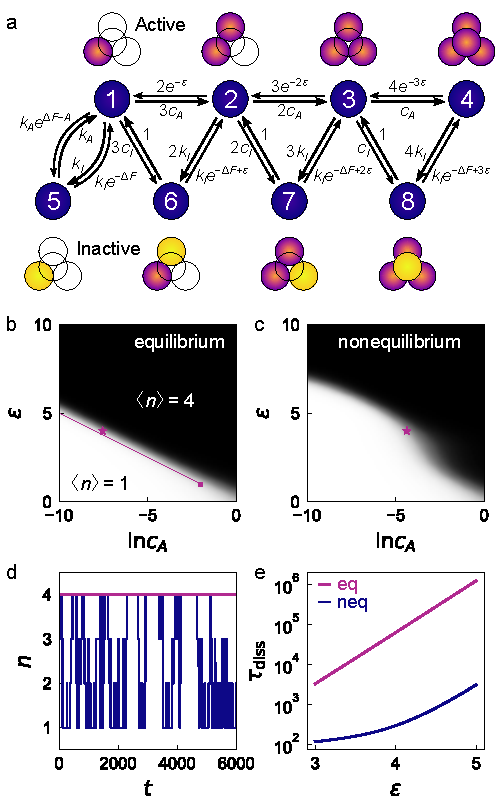
\includegraphics{figures/A5_BuildingStructures.pdf}
    \caption{\textbf{Building Structures.} (a) Markov network for the dissipative self-assembly of a tetrahedral cluster. The purple, yellow, and open circles represent ``active'' particles, ``inactive'' particles, and unoccupied sites, respectively. (b) Equilibrium phase diagram based on states 1 to 4. The grayscale map denotes the average occupancy of the cluster, $\langle n\rangle$. The solid line and the square marker denote the phase boundary and the critical point, respectively, in the thermodynamic limit of large clusters. (c) Nonequilibrium phase diagram for parameters $\Delta F=6$, $\ln c_I = -6$, and $k_I = 0.01$.  (d) Fluctuating occupancy $n$ for the equilibrium (purple) and nonequilibrium (blue) systems for an interaction strength $\varepsilon=4$ at phase coexistence (star markers in a and b). (e) Mean first passage time $\tau_{\text{diss}}$ from the assembled to the disassembled state ($4\rightarrow1$) for the equilibrium (purple) and nonequilibrium (blue) systems as a function of the interaction strength $\varepsilon$. }
    \label{fig:BuildingStructures}
\end{figure}
%%%%%%%%%%%%%%%%%%%%%%%%%%

Given that it costs a steady supply of energy to maintain disequilibrium in the active particle concentration, what is the benefit? In short, the answer is speed in assembling and/or disassembling particle structures. To show this, consider that the active particles interact with one another through attractive, short ranged interactions with a free energy gain $\varepsilon$ for each pairwise bond formed. We will assume that inactive particles do not interact with each other or the active particles. As summarized by the Markov network in Figure \ref{fig:BuildingStructures}a, active particles are added to the growing cluster with a diffusion-limited rate $k_{\text{on}} c_A$.  Active particles within the cluster become inactive with a rate $k_I$ and detach from the cluster at a rate $k_{\text{off}}$.  We set $k_{\text{on}}$ and $k_{\text{off}}$ equal to unity, such that time is measured in units of $k^{-1}_{\text{off}}$ and concentration in units of $k_{\text{off}}/k_{\text{on}}$.

Figures \ref{fig:BuildingStructures}b and \ref{fig:BuildingStructures}c compare the equilibrium phase behavior to that of the active system.  For the equilibrium assemblies, we consider only states 1 to 4 and plot the average number of particles within the cluster $\langle n\rangle$ as a function of the monomer concentration $c_A$ and the interaction energy $\varepsilon$.  For strong interactions or high monomer concentrations, the clusters are fully occupied $\langle n\rangle\rightarrow 4$ (Fig.~\ref{fig:BuildingStructures}b, black region).  For weak interactions or low monomer concentrations, the particles do not assemble $\langle n\rangle \rightarrow 1$ (Fig.~\ref{fig:BuildingStructures}b, white region).  Below the critical point (Fig.~\ref{fig:BuildingStructures}b, purple circle), coexistence of the assembled and disassembled states is reasonably well approximated by the thermodynamic result, $\varepsilon = -2\ln c_A$, which describes the limit of large clusters $N\rightarrow\infty$ \cite{marsland2018active}.  Driving the system away from equilibrium acts to perturb the coexistence boundary; however, the qualitative features of the phase diagram are similar to those at equilibrium (Fig.~\ref{fig:BuildingStructures}c). 

The dynamics of the two systems, however, are dramatically different.  For coexistence at equilibrium (i.e., when $p_1=p_4$), the characteristic time required to disassemble the tetrahedral cluster scales as $\tau_{\text{diss}}\sim e^{3\varepsilon}$.  The rate limiting step is the removal of one particle from the cluster ($4\rightarrow 3$), which results in the loss of three interparticle bonds.  For strong interactions ($\varepsilon\gg1$), the time scales required for assembly and disassembly become quite large.  By contrast, the dissipative structure has an alternate route for disassembly ($4\rightarrow 8\rightarrow 3$), which can be orders of magnitude faster than that of the equilibrium structure.  Figure \ref{fig:BuildingStructures}d shows the fluctuating occupancy of the cluster at coexistence for both the equilibrium and active systems with a common interaction energy of $\varepsilon=4$.  During this time period, the equilibrium system remains in the assembled state while the active system assembles and disassembles repeatedly.  The characteristic time for disassembly---defined as the mean passage time from state 4 to 1---is more than two orders of magnitude smaller for the active system than the equilibrium system (Fig.~\ref{fig:BuildingStructures}e). 

%%%%%%%%%%%%%%%%%%%%%%%%%%
\subsubsection{Dissipative Self-Assembly of Synthetic Materials}

Inspired by the cell cytoskeleton, the dissipative self-assembly of supramolecular materials has emerged as a promising strategy for controlling material organization in time as well as space \cite{VanRossum2017, De2018}. In contrast to equilibrium assemblies, where the rates of assembly and disassembly are related by detailed balance, dissipative self-assembly uses two or more processes to independently control the rates at which structures grow and degrade.  This basic concept has been applied to create a growing variety of supramolecular polymers \cite{Sorrenti2017} that exhibit simultaneous growth and shrinkage \cite{boekhoven2015transient}, tunable lifetimes \cite{Tena-Solsona2017}, conformational switching \cite{dhiman2017transient}, and nonequilibrium fluctuations \cite{boekhoven2015transient} reminiscent of dynamic instability in microtubules. In one pioneering study, small molecule building blocks were activated for assembly by reaction with a chemical fuel and subsequently degraded to their original inactive form by a different reaction pathway (Fig.~\ref{fig:BuldingStructure2}a) \cite{boekhoven2015transient}. As in the model above, the breaking of detailed balance enabled the formation of supramolecular assemblies that exhibit ``low-temperature'' phase behavior with ``high-temperature'' kinetics \cite{marsland2018active}.  Active soft matter with tunable lifetimes may be useful as self-erasing inks or as self-destructing hydrogels for tissue regeneration or drug release \cite{Rieß2018}.

%%%%%%%%%%%%%%%%%%%%%%%%%%
\begin{figure}[h!]
    \centering
    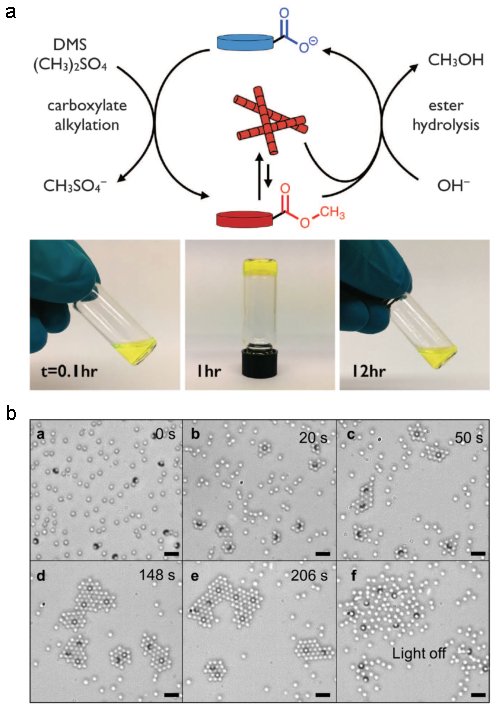
\includegraphics[width=8.5cm]{figures/A5_BuildingStructures2.pdf}
    \caption{(a) The dissipative  self-assembly of supramolecular materials forming the transient structure. Up: In a typical reaction cycle, carboxylate groups on the inactive self-assembling building blocks  react with the fuel, DMS, to produce methyl esters. These activated building blocks self-assemble into fibrous structures. Methyl esters can hydrolyze both in the assembled and free states to revert to the original inactive building block. One full cycle produces $CH_3OH$ (methanol) and $CH_3SO_4$(MMS) as waste products. Bottom: A typical sample in a reaction cycle at t = 0.1, 1, and 12 hours, with 1 mM of fluorescein added for coloring. \kbnote{(Adapted from Ref.~\cite{boekhoven2015transient} with permission.)}  (b) Photo-switchable assembly of a colloidal structure. A sequence of images showing the growth of crystals under full UV illumination. Active particles can be distinguished from the passive ones by the dark crescent or ring at their edge. Crystals melt by thermal diffusion when the light is turned off. \kbnote{(Adapted from Ref.~\cite{Singh2017} with permission.)} }
    \label{fig:BuldingStructure2}
\end{figure}
%%%%%%%%%%%%%%%%%%%%%%%%%%

In addition to molecular building blocks, the formation of dissipative structures by breaking detailed balance can also be applied to photoswitchable nanoparticles \cite{klajn2007light, kundu2015light, manna2015orthogonal, he2016light} and active colloids \cite{Soto2014, soto2015self, Niu2017, Singh2017, Schmidt2018} (Fig.~\ref{fig:BuldingStructure2}b). A particularly illustrative example is provided by a class of colloidal assemblies dubbed active colloidal molecules \cite{Lowen2018}, in which colloidal particles move due to concentration gradients created by themselves and their neighbors \cite{Soto2014}.  These dissipative structures appear to violate action-reaction symmetry---for example, two otherwise stationary particles may come together to form a stable, self-propelled cluster \cite{Soto2014}.  These and other motions are sustained by the steady supply or removal of chemical species at the particle surface (e.g., due to a catalytic reaction \cite{Singh2017} or release from the particle interior \cite{Niu2017}).  Interestingly, these dissipative assemblies are predicted to exhibit time-dependent functionality such as oscillatory deformations and run-and-tumble propulsion \cite{soto2015self}.  More generally, this example highlights the importance of feedback between structures and processes necessary for creating dynamic functions (Fig.~\ref{fig:1}b). Colloidal particles move in response to chemical gradients they create, and the gradients in turn are shaped by the particle configuration.  Beyond colloids, this basic strategy was recently employed to create acoustic metamaterials with dynamically tunable bandgaps \cite{bachelard2017emergence, bishop2017acoustic}; other realizations of dissipative self-assembly are sure to follow. 

%%%%%%%%%%%%%%%%%%%%%%%%%%
\subsection{Making Copies}

The dynamic functions of living matter trace their origins to the single function of ``making copies'', which provides the basis for evolution by natural selection.  Replication of the genetic code by molecular machines---namely, DNA polymerase---occurs with incredible fidelity characterized by an error rate of as small as $10^{-9}$ \cite{McCulloch2008}. This level of precision is critical in avoiding deleterious mutations, which can lead to improper function and even death of the organism. It has long been recognized that making such accurate copies requires energy dissipation \cite{Bennett1979}; however, the details of the dissipation-error trade-off depend on the specific proofreading mechanism \cite{Sartori2013}. DNA replication is but one important part of cellular reproduction, whereby the living cell creates a copy of itself---including both its internal structures and processes.  Here, we consider the comparably simple problem of creating a self-replicating material structure that contains some minimal amount of combinatorial information. We present a model for the self-replication of DNA origami rafts inspired by the experiments of Seeman and Chaikin \cite{He2017} (Fig.~\ref{fig:MakingCopies}) and discuss other routes toward the realization of self-replicating, evolvable matter.

%%%%%%%%%%%%%%%%%%%%%%%%%%
\subsubsection{A minimal replicator}

In the model, two monomers $A$ and $T$ can combine to form four possible dimers $AA$, $AT$, $TA$, and $TT$, each of which catalyzes its own formation.  We focus our attention on a particular dimer $AT$ and its function as a catalyst for the production of itself and the other `mutant' dimers (Fig.~\ref{fig:MakingCopies}a). During a successful replication cycle, the monomers $A$ and $T$ present in solution first bind to the seeded $AT$ template through complementary interactions.  Once bound, the monomers react to form a new $AT$ dimer that dissociates from the template to complete the cycle.  In addition to this ``correct'' cycle, we consider one of the ``incorrect'' cycles that leads to formation of the mutant $TT$; other types of errors are excluded to simplify the analysis.  The resulting model is described by a 6-state Markov network containing two cycles with currents $J_c$ and $J_i$ that quantify the production of the correct and incorrect dimers, respectively (Fig.~\ref{fig:MakingCopies}b).  In assessing replicator performance, we examine how the rate of copying $J_c$ and the error fraction $\eta = J_i/J_c$  depend on the dissipation rate. 

%%%%%%%%%%%%%%%%%%%%%%%%%%
\begin{figure}[h!]
    \centering
    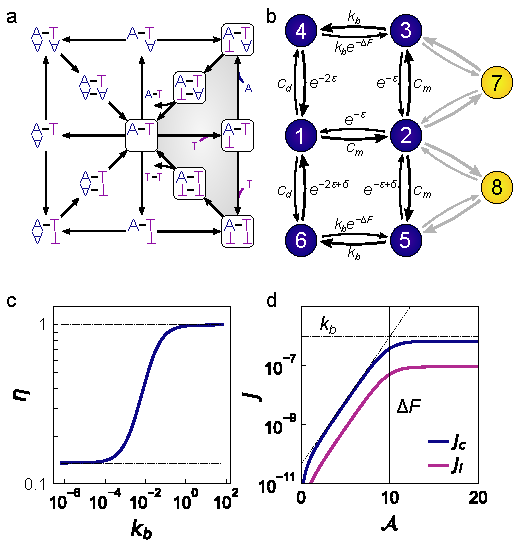
\includegraphics{figures/A5_MakingCopies.pdf}
    \caption{\textbf{Making Copies.}(a) Reaction network showing dimer formation catalyzed by the $AT$ template. (b) Markov network and transition rates corresponding to the shaded region of the network in (a). The additional states 7 and 8 correspond to a simple kinetic proofreading scheme. (c) Error fraction $\eta$ as a function of the bonding rate $k_b$ for $\Delta F = 10$, $\varepsilon = 6$, and $\delta=2$. For $k_b\ll e^{-\varepsilon+\delta/2}$, the error rate approaches its minimal value of $\eta=e^{-\delta}$. (d) Rate of formation for correct and incorrect dimers, $J_c$ and $J_i$, as a function of the driving affinity $\mathcal{A}$ for $c_m=e^{-4}$; other parameters are listed in (c). }
    \label{fig:MakingCopies}
\end{figure}
%%%%%%%%%%%%%%%%%%%%%%%%%%

In the model, monomers and dimers bind to the template with diffusion limited rates proportional to their respective concentrations in solution, $c_m$ and $c_d$ (Fig.~\ref{fig:MakingCopies}b). The rates of dissociation depend on the interaction energies, denoted $\varepsilon$ for $AT$ and $\varepsilon-\delta$ for $TT$. These monomer interactions combine in an additive fashion to determine the binding energy between two dimers. Bond formation between the bound monomers occurs at a rate $k_b$ with a free energy of reaction $\Delta F$.  Assuming equal concentrations of $AT$ and $TT$ dimers in solution, the driving affinity is $\mathcal{A} = 2\ln(c_m/c_d) + \Delta F$ for both the correct and incorrect replication cycles.  We assume that the bond energy is sufficiently large to inhibit spontaneous degradation of the dimers, $\Delta F\gg1$; the monomer binding energies are smaller by comparison such that $\Delta F> \varepsilon>\delta >0 $.

To minimize replication errors, the rate of bond formation should be sufficiently slow such that monomers equilibrate onto the catalyst template $AT$---that is, $k_b\ll e^{-\varepsilon + \delta/2}$ (Fig.~\ref{fig:MakingCopies}c). Under these conditions, the error fraction approaches $\eta = e^{-\delta}$ where $\delta$ is the difference in the binding energies of the correct and incorrect monomers.  If we operate in this high accuracy regime, a finite driving affinity is required to drive replication at a rapid rate (Fig.~\ref{fig:MakingCopies}d).  Optimal performance requires that monomers bind ($c_m>e^{-\varepsilon}$) while dimers unbind ($c_d<e^{-2\varepsilon}$), which implies large affinities, $\mathcal{A}>\Delta F$.  The model suggests that fast and accurate replication proceeds at a rate $J_c\sim k_b\ll e^{-\varepsilon+\delta/2}$ and dissipates at least $\Delta F$ per cycle. 

Additional energy input can allow for further improvements to replication accuracy through various forms of kinetic proofreading \cite{Hopfield1974, Murugan2012}.  In its simplest form, we consider two additional states---denoted 7 and 8---in which the $AT:T$ complex binds to modified monomers $A^*$ and $T^*$, respectively (Fig.~\ref{fig:MakingCopies}b). Once bound, the modified monomers convert to their native forms $A$ and $T$ prior to bond formation.  Steady currents around the proofreading cycles ($2\rightarrow7\rightarrow3$ and $2\rightarrow8\rightarrow5$) are powered by cycle affinities $\mathcal{A}_p$ due to the chemical potential difference between the modified and unmodified monomers in the surrounding reservoir.  By engineering the transition rates along these auxiliary cycles, the error fraction can be reduced to a minimum value of $\eta\rightarrow e^{-2\delta}$ \cite{Hartich2015}. Further improvements can be achieved using increasingly sophisticated proofreading networks \cite{Murugan2012}.

%%%%%%%%%%%%%%%%%%%%%%%%%%
\subsubsection{Self-replicating materials}

The pursuit of material structures capable of self-replication is motivated by the promise of revolutionary advances in materials synthesis and design \cite{He2017}. Given sufficient resources, the number of self-replicating structures grows exponentially with time thereby accelerating rates of material synthesis.  Perhaps more importantly, the ability to direct the evolution of replicating materials through application of selective pressures could facilitate the design of complex structures with desired functions.  At the molecular scale, the study of self-replication has long sought to provide useful insights into the chemical origins of life itself \cite{Orgel1992,ruiz2013prebiotic}. In this context, it is useful to distinguish self-replication of combinatorial information from simpler forms of autocatalysis that copy a single structure (not one of many possible structures) \cite{schulman2012robust}. Several mechanisms for autocatalysis have been explored including template-based copying \cite{Wang2011, He2017},  crystal growth and fragmentation \cite{Viedma2005,carnall2010mechanosensitive}, and catalytic reaction networks (hypercycles) \cite{Eigen1977, Zeravcic2014}. Combined with combinatorial information such as heterogeneous polymer sequences or macromolecular assemblies (Fig.~\ref{fig:MakingCopies2}a) \cite{sadownik2016diversification}, any form of autocatalysis with sufficient fidelity \cite{Eigen1988} can enable the creation of self-replicating materials.

Materials based on DNA \cite{Jones2015} possess several attributes useful in the development of self-replicating structures \cite{Wang2011, schulman2012robust, He2017}.  First, large amounts of combinatorial information can be encoded within sequences of nucleotide bases. Second, the specific interactions between complementary base pairs enables the programmable folding and assembly of complex structures.  These specific interactions of tunable strength can also be used to achieve autocatalysis via template-based copying \cite{Wang2011, He2017}.  In a recent work, Seeman and Chaikin showed how the replication of DNA origami rafts can lead to exponential growth with more than 7,000,000-fold amplification of the original seeded structure \cite{He2017}.  Strong, specific monomer-template interactions resulted in high fidelity copies but required cyclic energy inputs to promote monomer binding (low temperature), bond formation (UV light), and dimer unbinding (high temperature) (Fig.~\ref{fig:MakingCopies2}b). While thermodynamically costly, such external cycles offer significant practical benefits in controlling the replication process.  Remarkably, the seeding of two competing structures led to exponential growth and selection of the ``fittest'' structure, as determined by the replicator environment (namely, the pH).

%%%%%%%%%%%%%%%%%%%%%%%%%%%%%%%%%
\begin{figure}[h]
    \centering
    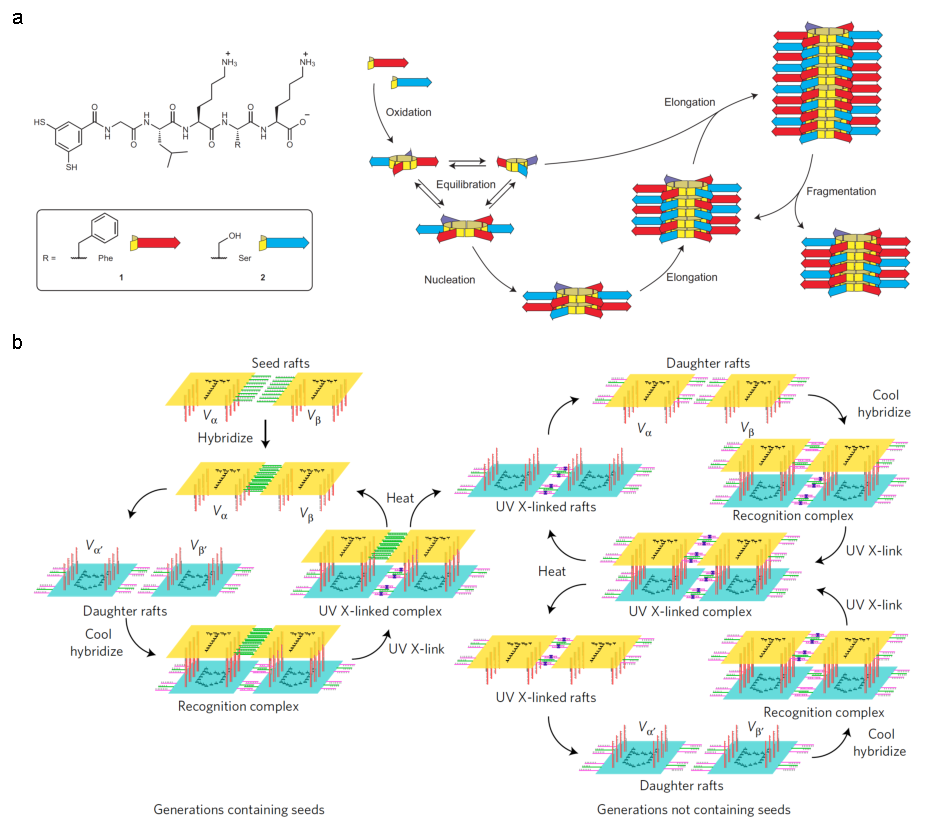
\includegraphics[width=8.5cm]{figures/A5_MakingCopies2.pdf}
    \caption{(a) Left: Structures of building blocks. Right: Mechanism of replication in a two-component system: the building blocks form an exchanging mixture of macrocycles of different sizes and building-block compositions via oxidation of thiols to give disulfide bonds and subsequent disulfide exchange. The hexamer macrocycles self-assemble into fibres as the peptide chains (arrows) form $\beta$-sheets through a nucleation–elongation mechanism. The fibres grow from their ends and break on mechanical agitation, which doubles the number of fibre ends that further promote the formation of self-replicating hexamer. \kbnote{(Adapted from Ref.~\cite{sadownik2016diversification} with permission.)} (c) Self-replication cycling of the dimer seed system, including ‘TT’ seed formation with special horizontal complementary sticky ends, recognition and hybridization of daughter rafts to seeds with two sets of vertical bonds ($V\alpha$ to $V\alpha^{'}$ , $V\beta$ to $V\beta^{'}$), formation of new-generation dimers using horizontal bonds and the $^{CNV} K$ photocrosslinking reaction and separation of the two successive generations by heating the system. The cycles on the left include seed rafts and those on the right do not. \kbnote{(Adapted from Ref.~\cite{He2017} with permission.)}  }
    \label{fig:MakingCopies2}
\end{figure}
%%%%%%%%%%%%%%%%%%%%%%%%%%%%%%%%%

Beyond DNA nanostructures, assemblies of micro- and nanoscale colloids interacting via DNA-based linkers \cite{leunissen2009towards}, magnetic dipoles \cite{zhang2014self, dempster2015self}, or toggled interactions \cite{zhang2014accelerated,sherman2016dynamic} are also promising candidates for self-replicating materials. The replication of 3D colloidal assemblies presents significant challenges for template-based copying strategies due to the presence of internal structural features that are inaccessible to components of the daughter structure.  One way around this challenge is to separate replication and assembly using flexible 1D assemblies, which unfold prior to replication and then reassemble into 3D structures \cite{cademartiri2014programmable}.  Alternatively, 3D clusters can be replicated with in larger catalytic networks in which structural features on one cluster template the formation of a second cluster and vice versa \cite{Zeravcic2014}.  Such catalytic cycles are predicted to emerge spontaneously within mixtures of colloidal spheres with specific time-varying interactions \cite{Zeravcic2017}.

%%%%%%%%%%%%%%%%%%%%%%%%%%
%%%%%%%%%%%%%%%%%%%%%%%%%%
\section{Conclusions}

The four dynamic functions considered here---keeping time, powering motion, building structures, and making copies---only begin to explore the diverse and creative solutions by which living organisms survive and thrive in complex non-equilibrium environments. In particular, we have largely omitted the discussion of functions related to computation and information processing, which remains an active area of statistical physics \cite{Parrondo2015, Lutz2015}. The ability to create material systems that sense their environment \cite{della2018fuel}, communicate with one another \cite{chen2013programmable}, and perform complex computations \cite{fang2016pattern} will benefit from an understanding of the fundamental connections between entropy and information. The creation of active soft matter on macroscopic scales will require careful consideration of transport processes, by which matter and energy are delivered to and removed from the material system. In biology, active transport mechanisms are favored over passive diffusion for length scales exceeding few microns \cite{soh2010reaction}. At larger scales, dissipative materials will likely benefit from the incorporation of synthetic vasculatures or other forms of active transport. The integration of multiple functions within material systems will require new levels of regulatory and control functions \cite{he2012synthetic} analogous to those of the living cell. Such functions are critical to realizing the full potential of soft robotics \cite{whitesides2018soft} to create ``life-like'' machines. It remains uncertain whether or not the capabilities of living matter will ever be matched by synthetic materials engineered to organize spontaneously and function autonomously. There is only one way to find out.
\end{appendices}

\end{document} 
